\documentclass[11pt,reqno]{amsart}

% ---------------------------------------------------------------------------
% Large-Wave Amplification on the Periodic Discrete Chain.
% Draft generated from the project notes (docs/) and the numerical certificates
% (numerics/).  Every theorem below is either proved here or verified numerically
% by the named script.  Bibliographic entries carry DOIs checked via Crossref where available;
% the Filimonov-group C. R. Acad. Sci. notes are cited from the lineage list of [F23].
% ---------------------------------------------------------------------------

\usepackage{amsmath,amssymb,amsthm}
\usepackage[margin=1in]{geometry}
\usepackage{graphicx}
\graphicspath{{figures/}}
\usepackage{booktabs}
\usepackage{longtable}
\usepackage{enumitem}
\usepackage{tikz}
\setlength{\emergencystretch}{4em}  % avoid overfull lines (long verify_*.py names have no break points)
\usetikzlibrary{decorations.pathmorphing}
\usepackage{hyperref}
\hypersetup{colorlinks=true,linkcolor=blue,citecolor=blue}

\theoremstyle{plain}
\newtheorem{theorem}{Theorem}
\newtheorem{lemma}[theorem]{Lemma}
\newtheorem{proposition}[theorem]{Proposition}
\newtheorem{corollary}[theorem]{Corollary}
\newtheorem{conjecture}[theorem]{Conjecture}
\theoremstyle{definition}
\newtheorem{remark}[theorem]{Remark}
\newtheorem{observation}[theorem]{Observation}

\newcommand{\Z}{\mathbb{Z}}
\newcommand{\Q}{\mathbb{Q}}
\newcommand{\R}{\mathbb{R}}
\newcommand{\C}{\mathbb{C}}
\newcommand{\LN}{L_N}
\newcommand{\eu}{\mathrm{e}}
\DeclareMathOperator{\circm}{circ}
\DeclareMathOperator{\rank}{rank}

\begin{document}

\title[Large-wave amplification on discrete lattices]{Large-wave amplification on periodic discrete lattices: linear theory and a nonlinear extension}
\author{Ilia Gradina}
\date{June 2026 (draft)}

\begin{abstract}
We study the large-wave effect for free oscillations of the periodic discrete chain
(the ring of $N$ beads) and for the discrete Schr\"odinger equation on the same ring.
Writing $A_N=\sup_{t}\max_j|u_j(t)|$ for the unit-impulse Green's function, we show that the
supremum is, by Bohr's theorem, the $\ell^1$ mass of the Fourier coefficients whenever the
frequencies $\{2\sin(\pi r/N)\}$ are linearly independent over $\Q$, and we prove this
independence for $N$ an odd prime and for $N=2^m$ by a cyclotomic argument. Consequently
$A_N=U_N:=\tfrac1{2N}\sum_{r=1}^{N-1}\csc(\pi r/N)=\tfrac1\pi\ln N+\tfrac1\pi(\gamma+\ln\tfrac2\pi)+o(1)$
unconditionally on these classes, and the same sharp constant holds for the composite family $N=2p$.
For every $N$ the upper bound $A_N\le U_N=\tfrac1\pi\ln N+O(1)$ is rigorous; the orbit-closure subtorus
has dimension exactly $\tfrac12\varphi(2N)$, and $A_N=U_N$ holds \emph{if and only if} every integer
relation among the frequencies has coefficient-sum divisible by four (with an antipodal variant for even
$N$)---an arithmetic criterion met by the prime and $2^m$ cases (and by no composite $N\le160$). A low-mode prefix gives strong evidence that $A_N=\Theta(\ln N)$ for
all $N$, which we leave as a conjecture, and we separate the infinite-time ceiling from the
finite-time (Diophantine) amplitude actually reached. For the discrete Schr\"odinger propagator
$\eu^{-\mathrm{i}t\LN}$, unitarity forbids amplification of a localized state, while the
$\ell^\infty\!\to\!\ell^\infty$ amplification satisfies $B_N=\Theta(\sqrt N)$ (upper bound from
unitarity, matching lower bound from a Bessel-front estimate). Proved results are separated throughout
from computational evidence and conjectures; all quantitative claims are reproduced by the accompanying
scripts.
\end{abstract}

\maketitle

\section{Introduction}

A localized disturbance on a homogeneous one-dimensional medium does not amplify: for the
continuous wave equation the classical bound of Zhukovsky gives $|\sigma(x,t)|\le F$~\cite{Zhukovsky}.
On the \emph{discrete} chain this is false~\cite{KMF,MF03,FM}. The discreteness of the spectrum, together
with the finiteness of the number of modes, allows many modes to come into phase and to produce a
local peak that grows with the number of nodes $N$. This is the \emph{large-wave effect}; related
phenomena include the splash effect~\cite{FMM} and its Schr\"odinger analogue~\cite{F23}.

The effect is genuinely discrete: it disappears in the continuum limit. The mechanism is the
\emph{finite, discrete spectrum}---finitely many discrete modes can be brought into near-coincidence of
phase (arbitrarily closely when their frequencies are rationally \emph{independent}, by Kronecker, and
otherwise as far as the relation lattice allows); on the infinite chain the spectrum is continuous, no exact
alignment occurs, and the amplification is absent. It is thus a finite-size spectral resonance rather than a
feature of the limiting partial differential equation. (For the discrete Schr\"odinger propagator the
absence of a continuum large wave is explicit: its single-site kernel is the Bessel function
$J_n(2t)$, whose peak over sites decays like $t^{-1/3}$, Section~\ref{sec:schr}.) This discrete--continuous gap,
together with the appearance of discrete Laplacians in quantum walks, photonic lattices, non-Hermitian
lattice optics~\cite{Longhi}, and discrete nonlinear models of anomalous (rogue) waves, motivates
studying the lattice in its own right.

\smallskip
\noindent\textbf{Contributions.} (i) We identify $\sup_t G_N(0,t)=U_N$ through Bohr's theorem under
rational independence of the frequencies (Section~3), and prove this independence for $N$ prime and
$N=2^m$ by a cyclotomic argument (Theorems~\ref{thm:prime},~\ref{thm:two}), giving the unconditional
asymptotics $A_N\sim\tfrac1\pi\ln N$ with the explicit constant of Lemma~\ref{lem:asym}; the same sharp
constant extends to the composite family $N=2p$ (Proposition~\ref{prop:2p}). (ii) For every
$N$ the upper bound $A_N\le U_N$ is rigorous, and we reduce $A_N$ \emph{exactly} to an optimization over
the orbit-closure subtorus, whose dimension we compute in closed form as $\tfrac12\varphi(2N)$
(Theorem~\ref{thm:qrank}); a sharp arithmetic criterion---coefficient-sums divisible by four (plus an antipodal variant for even
$N$)---decides exactly when $A_N=U_N$ (Theorem~\ref{thm:ceiling}), while a $\Q$-independent low-mode prefix gives strong
numerical evidence, but not yet a proof, that $A_N=\Theta(\ln N)$ in general (Conjecture~\ref{conj:order}).
(iii) For composite $N$ the value is algebraic with increasing arithmetic complexity
(Proposition~\ref{prop:closed}); we further separate the infinite-time ceiling from the finite-time
amplitude and show both the finite-horizon recurrence time and the effect of mass disorder
(Section~\ref{sec:reach}). (iv) For the discrete Schr\"odinger equation a localized state is never
amplified (unitarity, rigorous), and the $\ell^\infty\!\to\!\ell^\infty$ norm satisfies
$B_N=\Theta(\sqrt N)$, both bounds rigorous (Theorems~\ref{thm:schr},~\ref{thm:schr-lower}). (v)~As a
nonlinear outlook we connect $\LN$
to the rogue-wave problem (Section~\ref{sec:rogue}): the discrete NLS
$\mathrm i\dot z=-\LN z+\gamma|z|^2z$ has $\LN$ as its linear part and the focusing NLS as its
continuum limit, and we verify the Peregrine rogue solution, the modulational-instability gain, and
the emergence of heavy-tailed amplitude statistics in sharp contrast with the platykurtic linear value
law. Every quantitative claim is reproduced by a standalone, version-controlled script.

\smallskip
\noindent\textbf{Relation to prior work.} The large-wave \emph{phenomenon}---that on the discrete bead
string a localized disturbance amplifies, growing without bound at bounded energy on suitable $N$---is
classical, due to the Kurchanov--Myshkis--Filimonov line of work~\cite{KMF,MF03,FM}, with the $\ln$-type
asymptotics on the Dirichlet segment first in~\cite{FM98} and sharpened in~\cite{MF03}, and the
Schr\"odinger analogue in~\cite{F23}. The
linear independence over $\Q$ of the frequencies for $N$ prime or $N=2^m$ is itself due to~\cite{KMF};
our Theorems~\ref{thm:prime},~\ref{thm:two} reprove it cyclotomically, and Theorem~\ref{thm:qrank}
subsumes it in a closed-form $\Q$-rank valid for \emph{every} $N$. The
lineage summarized in~\cite{F23} also includes two early C.~R.~Acad.~Sci.\ notes on the bead
string~\cite{FKM91,F92}---in particular Filimonov's \emph{multiple-frequency} case~\cite{F92}, which bears
directly on the rational frequency dependencies studied here---which we have not been able to consult
directly (short notes, not digitized in the sources available to us); the structural claims below are
therefore stated as novel \emph{to our knowledge}, and~\cite{F92} should be compared against
Theorem~\ref{thm:ceiling} before submission.
Our contribution is \emph{quantitative and structural}: the explicit ring constant $\tfrac1\pi$ and the
next term $-\tfrac{\pi}{72}N^{-2}$ (Lemma~\ref{lem:asym}); the closed-form subtorus dimension
$\tfrac12\varphi(2N)$ for every $N$, with a cyclotomic reproof of the prime/$2^m$ independence
of~\cite{KMF} as its full-rank case (Theorems~\ref{thm:qrank},~\ref{thm:prime},~\ref{thm:two}); the exact $\bmod\,4$ criterion for reaching
the ceiling (Theorem~\ref{thm:ceiling}); the new composite family $N=2p$ (Proposition~\ref{prop:2p}); the
spectral-zeta systematization; the finite-time/disorder dichotomy (Section~\ref{sec:reach}); and the
sharp $B_N=\Theta(\sqrt N)$ growth of the discrete Schr\"odinger propagator
(Theorem~\ref{thm:schr-lower}). We do not claim the amplification effect itself as new.

\smallskip
\noindent\fbox{\parbox{0.97\linewidth}{\textbf{Main results at a glance.}
\begin{itemize}[leftmargin=1.4em,itemsep=1pt,topsep=2pt]
\item[\textbf{T1}] $A_N=U_N=\tfrac1\pi\ln N+\tfrac1\pi(\gamma+\ln\tfrac2\pi)-\tfrac{\pi}{72N^2}+\cdots$
for $N$ prime and $N=2^m$ (independence); $A_N=U_N-O(1/N)$ with the same constant $\tfrac1\pi$ for $N=2p$
(Thms.~\ref{thm:prime},~\ref{thm:two}, Prop.~\ref{prop:2p}).
\item[\textbf{T2}] The orbit-closure subtorus has dimension $\tfrac12\varphi(2N)$ for \emph{every} $N$
(Thm.~\ref{thm:qrank}).
\item[\textbf{T3}] \emph{Ceiling criterion}: $A_N=U_N$ iff every integer frequency relation has
coefficient-sum $\equiv0\ (\mathrm{mod}\ 4)$ (or, $N$ even, an antipodal variant; Thm.~\ref{thm:ceiling});
no composite $N\le160$ saturates, so there $\{N:A_N=U_N\}=\{\text{prime}\}\cup\{2^m\}$. Whether any
composite saturates is open (Cor.~\ref{cor:density}).
\item[\textbf{T4}] Discrete Schr\"odinger: localized states never amplify (unitarity), yet
$B_N=\Theta(\sqrt N)$ in $\ell^\infty$ (Thms.~\ref{thm:schr},~\ref{thm:schr-lower}).
\item[\textbf{T5}] The incoherent \emph{ceiling} has critical spectral dimension $d_s=1$ (incl.\ quasi-1D);
reachability there is the same open arithmetic question, and the amplitude is an infinite-time,
Diophantine-limited quantity (\S\ref{sec:dim},~\S\ref{sec:reach}).
\item[\textbf{C}] \emph{Open:} $A_N=\Theta(\ln N)$ for \emph{all} $N$ (Conj.~\ref{conj:order})---numerically
$A_N/\ln N\in[0.28,0.34]$ throughout.
\end{itemize}}}

We treat the periodic chain (the ring) with \emph{free} oscillations, and contrast it with the
discrete Schr\"odinger dynamics on the same ring. The central quantity is
\[
  A_N=\sup_{t\ge0}\ \max_{0\le j<N}|u_j(t)|,
\]
where $u_j(t)$ is the response to a unit velocity impulse. Our tools are the theory of
almost-periodic functions (Bohr), equidistribution (Kronecker--Weyl), and the arithmetic of
cyclotomic fields. The main message is that $A_N$ grows like $\ln N$, that the growth constant is
exactly $1/\pi$ on an explicit family of $N$, and that the obstruction on the remaining $N$ is a
purely number-theoretic one (rational relations among the frequencies).

\part{Linear theory}

% Part I -- Linear theory
% Included from large-wave-effect.tex; preamble macros (\LN, \Q, \eu, ...),
% \graphicspath and the bibliography all live in the root file.

\section{Toeplitz and circulant matrices: a unified language}\label{sec:setting}

The bead chain is a spring--mass lattice whose stiffness operator is shift invariant---hence
Toeplitz---and, under periodic boundary conditions, circulant (Figure~\ref{fig:chains}). We collect
the structures and the classical algorithms that organize the entire analysis.

\begin{figure}[ht]\centering
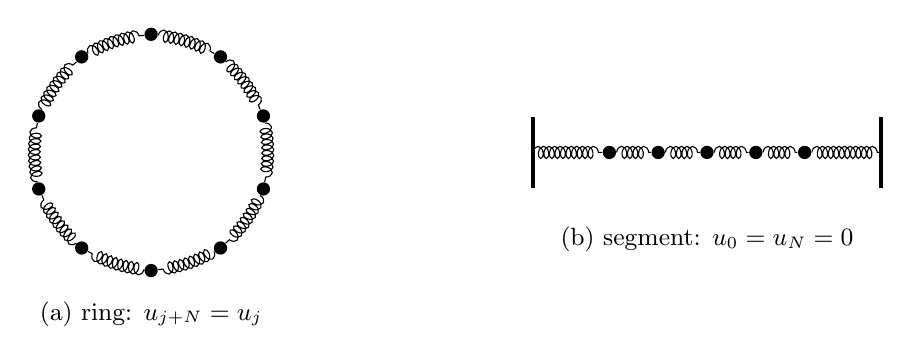
\begin{tikzpicture}[
  bead/.style={circle,fill=black,inner sep=1.7pt},
  spring/.style={decorate,decoration={coil,aspect=0.6,segment length=2pt,amplitude=2.2pt}}]
% (a) ring
\begin{scope}
  \def\R{1.5}
  \foreach \i in {0,...,9}{\node[bead] (b\i) at ({90-36*\i}:\R){};}
  \foreach \i [evaluate=\i as \j using {int(mod(\i+1,10))}] in {0,...,9}
    {\draw[spring] (b\i) to[bend left=10] (b\j);}
  \node at (0,-\R-0.55){\small (a) ring: $u_{j+N}=u_j$};
\end{scope}
% (b) segment
\begin{scope}[xshift=5.2cm,yshift=0cm]
  \draw[very thick] (-0.35,-0.45) -- (-0.35,0.45);
  \draw[very thick] ({6*0.62+0.35},-0.45) -- ({6*0.62+0.35},0.45);
  \foreach \i in {1,...,5}{\node[bead] (s\i) at (\i*0.62,0){};}
  \draw[spring] (-0.35,0) -- (s1);
  \foreach \i [evaluate=\i as \j using {int(\i+1)}] in {1,...,4}{\draw[spring] (s\i) -- (s\j);}
  \draw[spring] (s5) -- ({6*0.62+0.35},0);
  \node at ({3*0.62},-1.1){\small (b) segment: $u_0=u_N=0$};
\end{scope}
\end{tikzpicture}
\caption{The two geometries. (a) The ring of $N$ beads coupled by identical springs gives a
\emph{circulant} Laplacian $\LN=\circm(2,-1,0,\dots,0,-1)$. (b) The Dirichlet segment gives the
\emph{tridiagonal Toeplitz} $T_N=\operatorname{tridiag}(-1,2,-1)$. Both have the same symbol
$f(\theta)=4\sin^2(\theta/2)$.}\label{fig:chains}
\end{figure}

\subsection{Toeplitz, Hankel, circulant}
A matrix is \emph{Toeplitz} if it is constant along diagonals, $A_{ij}=a_{i-j}$ ($2n-1$ scalars,
$O(n)$ storage); \emph{Hankel} if constant along anti-diagonals, $H_{ij}=h_{i+j}$; and
\emph{circulant} if Toeplitz with a periodic wrap, $C_{ij}=c_{(i-j)\bmod n}$. For $n=4$,
\[
T=\begin{pmatrix}a_0&a_{-1}&a_{-2}&a_{-3}\\ a_1&a_0&a_{-1}&a_{-2}\\
a_2&a_1&a_0&a_{-1}\\ a_3&a_2&a_1&a_0\end{pmatrix},\quad
H=\begin{pmatrix}h_0&h_1&h_2&h_3\\ h_1&h_2&h_3&h_4\\ h_2&h_3&h_4&h_5\\ h_3&h_4&h_5&h_6\end{pmatrix},\quad
C=\begin{pmatrix}c_0&c_3&c_2&c_1\\ c_1&c_0&c_3&c_2\\ c_2&c_1&c_0&c_3\\ c_3&c_2&c_1&c_0\end{pmatrix}.
\]
Reversing rows turns Toeplitz into Hankel, $H=JT$ with $J$ the exchange matrix; a Toeplitz matrix is
the finite compression of a convolution (Laurent) operator. The ring Laplacian
$\LN=\circm(2,-1,0,\dots,0,-1)$ is the periodic case of the segment Toeplitz
$T_N=\operatorname{tridiag}(-1,2,-1)$.

\subsection{The symbol and circulant diagonalization}
A banded Toeplitz/circulant matrix with entries $a_k$ has \emph{symbol}
$f(\theta)=\sum_k a_k\eu^{\mathrm{i}k\theta}$; for both $\LN$ and $T_N$,
\[ f(\theta)=2-2\cos\theta=4\sin^2(\theta/2). \]
Every circulant is a polynomial $C=\sum_k c_k P^k$ in the cyclic shift $P$, and the Fourier modes
$\varphi^{(r)}_j=N^{-1/2}\eu^{2\pi\mathrm{i}rj/N}$ are common eigenvectors of $P$
($P\varphi^{(r)}=\eu^{2\pi\mathrm{i}r/N}\varphi^{(r)}$). Hence
\begin{equation}\label{eq:diag}
  \LN=F_N^\ast\Lambda F_N,\qquad
  \lambda_r=f\!\left(\tfrac{2\pi r}{N}\right)=4\sin^2\tfrac{\pi r}{N},\qquad
  \omega_r=\sqrt{\lambda_r}=2\sin\tfrac{\pi r}{N},
\end{equation}
$r=0,\dots,N-1$. The discrete dispersion relation $\omega(\theta)=2|\sin(\theta/2)|$ is literally the
square root of the symbol, sampled at $\theta=2\pi r/N$ on the ring and at $\theta=\pi k/(N{+}1)$ on
the segment ($\lambda^{\mathrm{Dir}}_k=4\sin^2\frac{\pi k}{2(N+1)}$). The twofold degeneracy
$\omega_r=\omega_{N-r}$ on the ring---absent on the segment---is the source of the arithmetic
difficulty in Section~\ref{sec:prime}.

\subsection{Classical Toeplitz algorithms}
Determined by $2n-1$ scalars, a Toeplitz system admits operations far below the dense $O(n^3)$
(Table~\ref{tab:toeplitz}); three enter the analysis.

\begin{table}[ht]\centering
\begin{tabular}{lll}
\toprule
Task & Algorithm & Cost \\
\midrule
Solve $Tx=b$ (symmetric) & Levinson (1947) & $O(n^2)$ \\
AR / Yule--Walker & Durbin (1960) & $O(n^2)$ \\
Inverse $T^{-1}$ (explicit) & Trench (1964) / Gohberg--Semencul (1972) & $O(n^2)$ \\
Multiply $Tx$, circulant solve, $f(\LN)$ & FFT / circulant embedding & $O(n\log n)$ \\
Semi-infinite chain & Wiener--Hopf factorization & --- \\
\bottomrule
\end{tabular}
\caption{Structured solvers used here; all beat the dense $O(n^3)$.}\label{tab:toeplitz}
\end{table}

\noindent\textbf{Levinson--Durbin.} For symmetric Toeplitz $R=(r_{|i-j|})$ the order-$i$ system
$R^{(i)}a^{(i)}=(r_1,\dots,r_i)^\top$ is built recursively through the \emph{reflection coefficients}
$k_i$ (PARCOR): with $E_0=r_0$,
\begin{equation}\label{eq:levinson}
  k_i=\frac{r_i-\sum_{j=1}^{i-1}a^{(i-1)}_j r_{i-j}}{E_{i-1}},\quad
  a^{(i)}_j=a^{(i-1)}_j-k_i\,a^{(i-1)}_{i-j},\quad a^{(i)}_i=k_i,\quad E_i=(1-k_i^2)E_{i-1}.
\end{equation}
Recursion~\eqref{eq:levinson} is due to Levinson~\cite{Levinson} and, in the AR (Yule--Walker) case,
Durbin~\cite{Durbin}; one has $|k_i|<1$ for all $i$ iff $R\succ0$, making $\{k_i\}$ the natural
stable-filter parametrization. The implementation used here goes back to the author's 2012
study~\cite{Gradina12} and is the AR core of the companion time-series work.

\noindent\textbf{Trench / Gohberg--Semencul.} The inverse of a Toeplitz matrix is \emph{not} Toeplitz
but is determined by its first and last columns $u,v$~\cite{Trench,GS} (two $O(n^2)$ recursions); writing $L_x,U_x$
for the lower/upper triangular Toeplitz matrices generated by a vector $x$,
\begin{equation}\label{eq:gs}
  T^{-1}=\tfrac1{u_0}\bigl(L_u U_{v}-L_{Sv}\,U_{Su}\bigr),
\end{equation}
a difference of products of triangular Toeplitz factors ($S$ the shift), with $\det T$ obtained en
route. On the ring this collapses to the pseudoinverse $\LN^{+}=F_N^\ast\Lambda^{+}F_N$ (the constant
mode, $\LN\mathbf1=0$, is mapped to $0$) and, more generally, $f(\LN)=F_N^\ast f(\Lambda)F_N$ in
$O(N\log N)$---the route by which the propagators below are evaluated.

\noindent\textbf{Wiener--Hopf.} On the semi-infinite chain the stiffness is a one-sided Toeplitz
operator; its inversion is the Wiener--Hopf factorization $f(\theta)=f_+(\theta)f_-(\theta)$ of the
symbol, which links the finite-$N$ ceilings to the operator-theoretic (Szeg\H{o}) asymptotics of
Section~\ref{sec:upper}.

\subsection{Three dynamics and the central functional}
The same lattice carries the wave equation $\ddot u+\LN u=0$ (propagator $\cos(t\sqrt{\LN})$), the
discrete Schr\"odinger equation $\mathrm i\dot z=\LN z$ (propagator $\eu^{-\mathrm i t\LN}$, the phase
governed by $\lambda_r$ rather than $\omega_r=\sqrt{\lambda_r}$), and the dissipative heat flow
$\dot v=-\LN v$ (no large wave---the semigroup smooths). For the wave equation with the unit zero-mean
velocity impulse $u(0)=0$, $\dot u(0)=e_0-\tfrac1N\mathbf 1$, the response is the velocity Green's
function
\begin{equation}\label{eq:green}
  u_j(t)=G_N(j,t)=\frac1N\sum_{r=1}^{N-1}\frac{\sin(\omega_r t)}{\omega_r}\,\eu^{2\pi\mathrm{i}rj/N}.
\end{equation}
As $u$ is real and $\omega_r=\omega_{N-r}$, \eqref{eq:green} is a real almost-periodic function of $t$
with frequency set $\{\omega_r\}$, and the large wave is the operator-norm growth
$A_N=\sup_t\max_j|G_N(j,t)|$.

\section{Bohr's supremum and the ceiling \texorpdfstring{$U_N$}{U\_N}}

\begin{proposition}[Bohr ceiling]\label{prop:bohr}
For every $N$ and every node $j$,
\(
  \sup_t|G_N(j,t)|\le U_N,\ U_N:=\tfrac1{2N}\sum_{r=1}^{N-1}\csc(\pi r/N),
\)
with equality at $j=0$ provided the frequencies $\{\omega_r:1\le r\le\lfloor N/2\rfloor\}$ are
linearly independent over $\Q$.
\end{proposition}

\begin{proof}
Grouping the degenerate pair $r,\,N-r$ gives, at $j=0$,
$G_N(0,t)=\sum_{r=1}^{\lfloor N/2\rfloor}b_r\sin(\omega_r t)$ with $b_r=2/(N\omega_r)>0$
(the term $r=N/2$, if present, has coefficient $1/(N\omega_{N/2})$). The triangle inequality
gives $|G_N(j,t)|\le\frac1N\sum_{r=1}^{N-1}\omega_r^{-1}=U_N$ for all $j$. If the $\omega_r$ are
$\Q$-independent, then by Kronecker--Weyl the orbit $\{(\omega_r t)_r\}$ is dense in the torus, so
$\sin(\omega_r t)\to1$ simultaneously and the bound is attained at $j=0$. (Bohr's theorem:
$\sup_t\sum b_r\sin(\omega_r t)=\sum|b_r|$.)
\end{proof}

\section{The exact constant}

\begin{lemma}[Euler--Maclaurin asymptotics]\label{lem:asym}
$\displaystyle U_N=\frac1\pi\Big(\ln N+\gamma+\ln\frac2\pi\Big)+o(1)
   =\frac1\pi\ln N+0.039\,99\ldots+o(1).$
\end{lemma}

\noindent The leading term comes from the singularity $\csc(\pi r/N)\sim N/(\pi r)$ at small $r$,
which yields the harmonic sum $\sum 1/r\sim\ln$; the constant follows from the Euler--Maclaurin
correction. Numerically $U_N-\tfrac1\pi\ln N\to0.03999$ for $N\le 65536$
(\texttt{numerics/verify\_lemma3\_lebesgue.py}).

\section{Upper bounds: energy and the Szeg\H{o} symbol}\label{sec:upper}

A fixed-energy bound caps the response. With energy
$E=\tfrac12\dot u^\top\dot u+\tfrac12 u^\top\LN u$ and the exact trigonometric identity (the cotangent
sum, derived in Section~\ref{sec:zeta})
\begin{equation}\label{eq:csc2}
  \sum_{r=1}^{N-1}\frac1{\sin^2(\pi r/N)}=\frac{N^2-1}{3},
\end{equation}
Cauchy--Schwarz on the modal expansion gives $\|u(t)\|_\infty\le C\sqrt N\,\sqrt E$: at fixed energy
the deflection cannot exceed order $\sqrt N$, a ceiling attained by the time-reversed focusing
configuration (the variational maximum; \texttt{verify\_theorem1.py}). The same sum yields the exact
pseudo-inverse diagonal $(\LN^{+})_{jj}=\tfrac1N\sum_{r\ne0}\lambda_r^{-1}=\tfrac{N^2-1}{12N}$.

Asymptotically the eigenvalues follow the symbol through Szeg\H{o}'s theorem~\cite{GrenanderSzego,Gray}:
for continuous $F$,
\begin{equation}\label{eq:szego}
  \frac1N\sum_{r=0}^{N-1}F(\lambda_r)\xrightarrow{N\to\infty}\frac1{2\pi}\int_0^{2\pi}F\bigl(f(\theta)\bigr)\,d\theta,
  \qquad f(\theta)=4\sin^2(\theta/2),
\end{equation}
so spectral sums such as $U_N$ and $(\LN^{+})_{jj}$ are Riemann sums of the symbol; the logarithmic
growth of $U_N$ is exactly the borderline (logarithmically divergent) singularity
$f^{-1/2}\sim|\theta|^{-1}$ at $\theta=0$. (Szeg\H{o}'s theorem
proper requires continuous $F$; the \emph{singular} sums $U_N=\tfrac1{2N}\sum\lambda_r^{-1/2}$ and
$(\LN^{+})_{jj}=\tfrac1N\sum\lambda_r^{-1}$ are made rigorous by Euler--Maclaurin at the band edge,
Appendix~\ref{app:bernoulli}, the singularity producing the logarithm and the $N^2$ growth.) The propagators
$\cos(t\sqrt{\LN})$, $\eu^{-\mathrm i t\LN}$, $\LN^{-1/2}\sin(t\sqrt{\LN})$ are functions of the matrix
in the sense of Golub--Van Loan~\cite{GVL}, evaluated exactly by \eqref{eq:diag}; this puts the
operator-norm functionals $\|f_t(\LN)\|_{\ell^p\to\ell^q}$ on a rigorous footing.

\section{The spectral zeta function and the large-wave constants}\label{sec:zeta}

Define the spectral zeta of the ring Laplacian (zero mode removed),
\begin{equation}\label{eq:zeta}
  \zeta_{\LN}(s)=\sum_{r=1}^{N-1}\lambda_r^{-s}=4^{-s}\sum_{r=1}^{N-1}\csc^{2s}\tfrac{\pi r}{N},
  \qquad \Re s>0 .
\end{equation}
At integer $s$ this is a cosecant power sum with a closed form in $N$ (Bernoulli numbers,
Appendix~\ref{app:bernoulli}); the first two are
\[
  \zeta_{\LN}(1)=\frac{N^2-1}{12},\qquad \zeta_{\LN}(2)=\frac{(N^2-1)(N^2+11)}{720}.
\]
The first is elementary: from the classical identity $\sum_{r=1}^{N-1}\cot^2\frac{\pi r}{N}=\frac{(N-1)(N-2)}3$
and $\csc^2=1+\cot^2$,
\[
  \sum_{r=1}^{N-1}\csc^2\tfrac{\pi r}{N}=(N-1)+\frac{(N-1)(N-2)}3=\frac{N^2-1}3,
  \qquad\text{so}\qquad \zeta_{\LN}(1)=\tfrac14\sum_{r}\csc^2\tfrac{\pi r}{N}=\frac{N^2-1}{12},
\]
and $\zeta_{\LN}(2)$ follows the same way from $\sum_r\csc^4=\frac{(N^2-1)(N^2+11)}{45}$ (all integer values
are even polynomials in $N$, \texttt{verify\_spectral\_zeta.py}).
The two large-wave constants are \emph{special values of this single object}:
\begin{equation}\label{eq:zeta-values}
  U_N=\frac{\zeta_{\LN}(1/2)}{N},\qquad M_N^2=\frac{2E_0\,\zeta_{\LN}(1)}{N},
\end{equation}
the first because $\csc(\pi r/N)=2\lambda_r^{-1/2}$, the second because $(\LN^{+})_{jj}=\zeta_{\LN}(1)/N$.
Thus the Bohr ceiling (the large wave, $A_N\sim U_N$) and the variational ceiling $M_N$
(Section~\ref{sec:upper}) are the values of $\zeta_{\LN}$ at $s=\tfrac12$ and $s=1$.

The two growth laws are then dictated by the analytic structure of $\zeta_{\LN}$. By Szeg\H{o}'s
theorem the normalized zeta converges to the symbol integral,
\begin{equation}\label{eq:zeta-density}
  \frac1N\,\zeta_{\LN}(s)\xrightarrow{N\to\infty}
  I(s)=\frac1{2\pi}\int_0^{2\pi}(2-2\cos\theta)^{-s}\,d\theta
  =\frac{4^{-s}\,\Gamma(\tfrac12-s)}{\sqrt{\pi}\,\Gamma(1-s)},\qquad \Re s<\tfrac12,
\end{equation}
which has a simple pole at $s=\tfrac12$ (Figure~\ref{fig:zeta}). The edge of convergence is exactly the
logarithmic singularity producing $U_N=\zeta_{\LN}(\tfrac12)/N=\tfrac1\pi\ln N+O(1)$ (Lemma~\ref{lem:asym}).
At $s=1$ the density diverges, and indeed $\zeta_{\LN}(1)\sim N^2/12$ yields the $\sqrt N$ variational
ceiling $M_N\sim\sqrt{N/6}$. \emph{The large wave sits precisely at the convergence edge $s=\tfrac12$ of
the limiting spectral density $I(s)$}; the finite-$N$ $\zeta_{\LN}$ is itself an entire finite sum, and
it is the $N\to\infty$ density that carries the pole. The finite-$N$ zeta is an Epstein/Hurwitz-type
object whose integer values are polynomials in $N^2$ and whose half-integer value carries the logarithm.
All identities are verified (\texttt{verify\_spectral\_zeta.py}). At the opposite end, the spectral
determinant is the $s=0$ \emph{derivative}: $\zeta_{\LN}'(0)=-\log\det{}'\LN$ with
$\det{}'\LN=\prod_{r\ne0}\lambda_r=N^2$ (from $\prod_{r=1}^{N-1}2\sin(\pi r/N)=N$), so by Kirchhoff's
matrix-tree theorem the cycle $C_N$ has exactly $\det{}'\LN/N=N$ spanning trees---a graph invariant read
off $\zeta_{\LN}'(0)$ (\texttt{verify\_spanning\_trees.py}).

\begin{figure}[ht]\centering
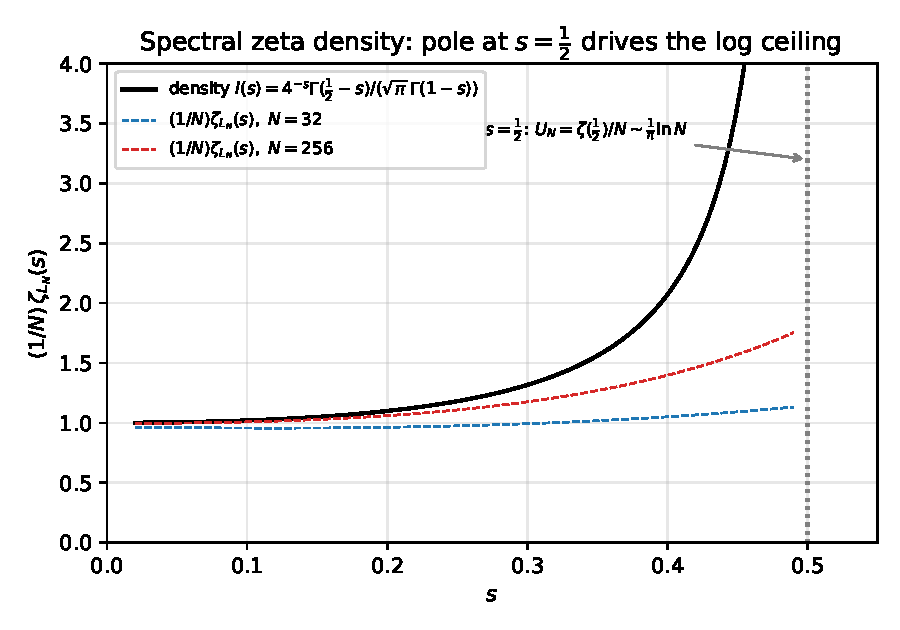
\includegraphics[width=.72\textwidth]{fig_zeta.pdf}
\caption{The normalized spectral zeta $\frac1N\zeta_{\LN}(s)$ converges to the symbol density $I(s)$ of
\eqref{eq:zeta-density}, which has a pole at $s=\tfrac12$. The large-wave ceiling is the boundary value
$U_N=\zeta_{\LN}(\tfrac12)/N\sim\tfrac1\pi\ln N$.}\label{fig:zeta}
\end{figure}

\section{Operator-norm hierarchy and the variational principle}\label{sec:opnorm}

The large wave is one corner of a hierarchy of operator norms of the velocity propagator
$S_N(t)=f_t(\LN)$ on the zero-mean subspace $\mathcal H_0=\{x\in\R^N:\sum_jx_j=0\}$, where
$f_t(\lambda)=\sin(t\sqrt\lambda)/\sqrt\lambda$ for $\lambda>0$ and $f_t(0)=0$ (circulant on
$\mathcal H_0$, kernel $G_N$; the constant mode is excluded since $\LN\mathbf1=0$). Its time-supremum in
different $\ell^p\to\ell^q$ norms obeys \emph{three distinct growth laws} (Table~\ref{tab:opnorm}, all
verified by \texttt{verify\_operator\_norms.py}):
\begin{equation}\label{eq:opnorm}
\begin{aligned}
  \sup_t\|S_N(t)\|_{2\to2}&=\frac1{2\sin(\pi/N)}\sim\frac{N}{2\pi},\\
  \sup_t\|S_N(t)\|_{2\to\infty}&\le\sqrt{\tfrac{\zeta_{\LN}(1)}{N}}\sim\sqrt{\tfrac N{12}},\\
  \sup_t\|S_N(t)\|_{1\to\infty}&=A_N\le U_N\sim\tfrac1\pi\ln N .
\end{aligned}
\end{equation}
\emph{Derivations.} $S_N(t)$ is symmetric with eigenvalues $f_t(\lambda_r)=\sin(t\omega_r)/\omega_r$, so
its $\ell^2\!\to\!\ell^2$ norm is $\max_r|\sin(t\omega_r)|/\omega_r$, whose supremum over $t$ is
$1/\omega_1=1/(2\sin\tfrac\pi N)$---the slowest mode reaching $\sin(t\omega_1)=\pm1$; this is exact and
unconditional. For $\ell^2\!\to\!\ell^\infty$, by translation invariance the norm is the $\ell^2$-length
of one row of $G_N$, and Parseval gives
\[
  \|G_N(\cdot,t)\|_2^2=\frac1N\sum_{r=1}^{N-1}\frac{\sin^2(t\omega_r)}{\omega_r^2}
  \ \le\ \frac1N\sum_{r}\omega_r^{-2}=\frac{\zeta_{\LN}(1)}N,
\]
hence $\sup_t\|S_N(t)\|_{2\to\infty}\le\sqrt{\zeta_{\LN}(1)/N}\sim\sqrt{N/12}$, with equality iff all
$\sin^2(t\omega_r)=1$ simultaneously---rational independence ($N$ prime, $2^m$). Finally
$\|S_N(t)\|_{1\to\infty}=\max_{j,k}|S_N(t)_{jk}|=\max_m|G_N(m,t)|$, whose time-supremum is, by definition,
$A_N\le\sum_r|a_r|=U_N$. The three corners thus read the spectral sums $\sum_r\omega_r^{-p}$ ($p=1,2$)
through different lenses; the $\ell^1\!\to\!\ell^\infty$ corner---weakest input, strongest output---is
precisely the large wave $A_N$.

\emph{Variational principle.} The energy norm has the direct reading: maximizing the deflection at a
node over the energy sphere $E(u_0,v_0)\le E_0$ on $\mathcal H_0$ is a constrained quadratic problem solved by Lagrange
multipliers,
\[
  \sup_{E(u_0,v_0)\le E_0}\ \max_j|u_j(t)| = \sqrt{2E_0\,(\LN^{+})_{jj}}=\sqrt{\tfrac{E_0(N^2-1)}{6N}}=M_N,
\]
\emph{independent of $t$} (the focusing configuration is the time-reversed peak). This is the
operator-norm/variational face of the energy ceiling, and via \eqref{eq:zeta-values} both $M_N$ and
$U_N$ are special values of the spectral zeta. The Szeg\H{o} symbol $f(\theta)=4\sin^2(\theta/2)$
controls all three norms through the spectral sums $\sum_r\omega_r^{-p}$.

\begin{table}[ht]\centering
\begin{tabular}{llll}
\toprule
norm & $\sup_t\|S_N(t)\|$ & growth & meaning \\
\midrule
$\ell^2\!\to\!\ell^2$ & $1/(2\sin\tfrac\pi N)$ & $N/2\pi$ & lowest-mode resonance \\
$\ell^2\!\to\!\ell^\infty$ & $\le\sqrt{\zeta_{\LN}(1)/N}$ & $\sqrt{N/12}$ & energy ceiling / variational $M_N$ \\
$\ell^1\!\to\!\ell^\infty$ & $A_N\le U_N=\zeta_{\LN}(1/2)/N$ & $\tfrac1\pi\ln N$ & \textbf{large wave} $A_N$ \\
\bottomrule
\end{tabular}
\caption{Three growth laws from one propagator. The $\ell^2\!\to\!\ell^2$ supremum is exact and
unconditional; the other two equal the listed ceilings on the $\Q$-independent classes $N$ prime and
$N=2^m$ (for $N=2p$, Proposition~\ref{prop:2p} gives only an $O(N^{-1})$ gap for the
$\ell^1\!\to\!\ell^\infty$ large wave) and are bounded by them in general. The large wave is the
$\ell^1\!\to\!\ell^\infty$ corner.}\label{tab:opnorm}
\end{table}

\section{Independence theorems and unconditional growth}\label{sec:prime}

\begin{theorem}[odd prime]\label{thm:prime}
Let $p$ be an odd prime. Then $\{\sin(\pi r/p):1\le r\le\tfrac{p-1}2\}$ is linearly independent
over $\Q$; hence $A_p=U_p\sim\tfrac1\pi\ln p$.
\end{theorem}

\begin{proof}
Put $\eta=\zeta_{2p}=\eu^{\mathrm{i}\pi/p}$. As $p$ is odd, $[\Q(\eta):\Q]=\varphi(2p)=p-1$, so
$\{1,\eta,\dots,\eta^{p-2}\}$ is a $\Q$-basis, and $\eta^{p}=\eu^{\mathrm{i}\pi}=-1$. From
$\eta^{-r}=\eta^{2p-r}=\eta^{p}\eta^{p-r}=-\eta^{p-r}$ we get $2\mathrm{i}\sin(\pi r/p)=\eta^r-\eta^{-r}=\eta^r+\eta^{p-r}$.
Suppose $\sum_{r=1}^{(p-1)/2}c_r\sin(\pi r/p)=0$ with $c_r\in\Q$. Then
$\sum_r c_r\eta^r+\sum_r c_r\eta^{p-r}=0$. As $r$ runs over $\{1,\dots,\tfrac{p-1}2\}$ the exponents
$r$ fill $\{1,\dots,\tfrac{p-1}2\}$ and $p-r$ fill $\{\tfrac{p+1}2,\dots,p-1\}$, together covering
$\{1,\dots,p-1\}$ bijectively, so $\sum_{m=1}^{p-1}d_m\eta^m=0$ with $d_m=c_m$ or $c_{p-m}$.
Finally $\Phi_{2p}(\eta)=\sum_{j=0}^{p-1}(-1)^j\eta^j=0$ gives $\eta^{p-1}=-\sum_{j=0}^{p-2}(-1)^j\eta^j$,
whose constant term is $-1\ne0$; equating coordinates in $\{1,\eta,\dots,\eta^{p-2}\}$ forces
$d_{p-1}=0$ and then all $d_m=0$, i.e. all $c_r=0$. The conclusion follows from
Proposition~\ref{prop:bohr}. \end{proof}

\begin{theorem}[powers of two]\label{thm:two}
For $N=2^m$, $\{\sin(\pi r/N):1\le r\le N/2\}$ is $\Q$-independent; hence $A_N=U_N\sim\tfrac1\pi\ln N$.
\end{theorem}

\begin{proof}
Now $\eta=\zeta_{2N}$, $\Phi_{2N}(x)=x^{N}+1$ (degree $\varphi(2N)=N$), so $\{1,\dots,\eta^{N-1}\}$ is a
basis and $\eta^{N}=-1$. Again $2\mathrm{i}\sin(\pi r/N)=\eta^r+\eta^{N-r}$, and for $1\le r\le N/2$ the
exponents $r$ and $N-r$ lie in $\{1,\dots,N-1\}$ \emph{without reduction}; they are distinct basis
powers (the index $N/2$ occurring with coefficient $2c_{N/2}$). Linear independence is immediate.
\end{proof}

An exact integer-rank certificate validates the prime case (\texttt{verify\_lemma1\_prime.py}); the
general rank formula is checked separately by \texttt{verify\_independence\_rank.py}.

\medskip\noindent\textbf{Worked example (prime $N=5$).} The two distinct frequencies
$\omega_1=2\sin36^\circ=1.1756$ and $\omega_2=2\sin72^\circ=1.9021$ stand in the ratio
$\omega_2/\omega_1=2\cos36^\circ=\varphi=\tfrac{1+\sqrt5}2$, the \emph{golden ratio}---irrational, so the
relation lattice is trivial ($\Lambda_5=\{0\}$) and Theorem~\ref{thm:prime} applies. The node-$0$ response
is the two-tone signal $G_5(0,t)=\tfrac25\bigl(\omega_1^{-1}\sin\omega_1 t+\omega_2^{-1}\sin\omega_2 t\bigr)$,
and by Kronecker both sines reach $1$ at a common near-alignment time, so
\[
  A_5=U_5=\tfrac15\bigl(\csc36^\circ+\csc72^\circ\bigr)=0.5506,
\]
the supremum equal to the ceiling, approached arbitrarily closely (in contrast to the composite $N=12$ below;
\texttt{verify\_exact\_AN.py}).

\begin{observation}[low-mode prefix]\label{obs:prefix}
Let $M(N)$ be the largest $M$ with $\{\sin(\pi r/N):r\le M\}$ $\Q$-independent; by Kronecker these modes
can be brought simultaneously into phase, contributing
$L_{\mathrm{pre}}(N)=\tfrac1N\sum_{r=1}^{M(N)}\csc(\pi r/N)$, which numerically satisfies
$L_{\mathrm{pre}}(N)\ge 0.25\,\ln N$ for all tested $N\le256$ (including the highly composite
$N=210,240$). This does \emph{not} by itself bound $A_N$ from below: the out-of-prefix modes may
interfere destructively, and controlling that interference is the open step.
\end{observation}

\begin{conjecture}[order, all $N$]\label{conj:order}
$A_N=\Theta(\ln N)$ for every $N$; more precisely $A_N\sim\tfrac1\pi\ln N$. This is proved for $N$ prime,
$N=2^m$, and $N=2p$ (Theorems~\ref{thm:prime}--\ref{thm:two}, Proposition~\ref{prop:2p}); for general
$N$ it is supported by Observation~\ref{obs:prefix} and by the exact subtorus computation of
Section~\ref{sec:exact}, where $A_N/\ln N$ stays in $[0.28,0.31]$ throughout the tested range
(\texttt{verify\_lemma4\_prefix.py}, \texttt{verify\_open\_problems.py}), but is not proved. The exact
saturation locus $A_N=U_N$ is settled by the arithmetic criterion of Theorem~\ref{thm:ceiling}; the open
content is the \emph{lower} order of $A_N$ on the non-saturating $N$.
\end{conjecture}

\subsection{The Dirichlet segment}\label{sub:segment}
The segment chain $\mathrm{tridiag}(-1,2,-1)$ with Dirichlet ends has the \emph{simple} spectrum
$\mu_k=2\sin\frac{\pi k}{2(N+1)}$ ($k=1,\dots,N$): no degeneracy, the structural advantage over the
ring, whose twofold $\mu_r=\mu_{N-r}$ halves the independent phases. Writing $\mu_k=2\sin(2\pi k/M)$ with
$M=4(N+1)$, the frequencies lie in $\Q(\zeta_M)$ with $2\mathrm{i}\sin(2\pi k/M)=\zeta_M^k-\zeta_M^{-k}$,
and the same minus-eigenspace argument gives the subtorus dimension
\begin{equation}\label{eq:segrank}
  \dim_\Q\operatorname{span}\{\mu_1,\dots,\mu_N\}=\min\!\bigl(N,\ \tfrac12\varphi(4(N+1))\bigr)
  \qquad(\text{verified for }N\le30,\ \text{conjectured in general}),
\end{equation}
which is full ($=N$, whence $A_N^{\mathrm{Dir}}=U_N^{\mathrm{Dir}}\sim\frac1\pi\ln N$ by Bohr)
when $N+1$ is prime or a power of two (and, assuming \eqref{eq:segrank}, only then)---the exact analogue of Theorems~\ref{thm:prime}--\ref{thm:two}
shifted by the boundary (the ring uses modulus $2N$, the segment $4(N+1)$). The $\Q$-independent low-mode
prefix again supports $A_N^{\mathrm{Dir}}=\Theta(\ln N)$ for every $N$ numerically, subject to the same
out-of-prefix gap as Conjecture~\ref{conj:order} (\texttt{verify\_segment\_lower\_bound.py}).

\section{Exact \texorpdfstring{$A_N$}{A\_N} for composite \texorpdfstring{$N$}{N}}\label{sec:exact}

For composite $N$ the frequencies satisfy rational relations and the orbit closure is a proper
\emph{subtorus} (Weyl). In the cyclotomic coordinates $C$ (row $r$ = integer coordinates of
$2\mathrm{i}\sin(\pi r/N)$ in $\Q(\zeta_{2N})$) the attainable phases are $\{\varphi=C\psi\}$, whence
\begin{equation}\label{eq:subtorus}
  \sup_t u_j(t)=\max_{\psi\in\R^p}\sum_r a_{rj}\sin\big((C\psi)_r\big),\qquad p=\varphi(2N),
\end{equation}
a finite-dimensional trigonometric maximization, reduced exactly and then evaluated numerically
(\texttt{verify\_exact\_AN.py}, returning $A_N=U_N$ on primes; a certified global bracket is given for
$N=6$ below). This makes the composite case computable for each $N$:
numerically the subtorus defect on the ring is $A_N/U_N\in[0.84,0.92]$ in the tested range, so
$A_N/\ln N\in[0.28,0.31]$, consistent with Conjecture~\ref{conj:order} ($A_N=\Theta(\ln N)$).

\begin{proposition}[algebraic composite cases]\label{prop:closed}
$A_N$ is an algebraic number: writing $x_r=\cos\varphi_r$, $y_r=\sin\varphi_r$ with $x_r^2+y_r^2=1$ and
adjoining, for each generator $k$ of the relation lattice $\Lambda$, the constraints
$\cos\langle k,\varphi\rangle=1$, $\sin\langle k,\varphi\rangle=0$ that cut out the orbit-closure subtorus
$\mathbb{T}_N$ (polynomials in the $x_r,y_r$ through the Chebyshev/addition formulas), turns
\eqref{eq:subtorus} into the maximum of a polynomial over a compact semialgebraic set defined over $\Q$,
whose value is algebraic by the Tarski--Seidenberg theorem (real quantifier elimination). For $N=6$ the relation lattice is one-dimensional and
\[
  A_6=\frac{\sqrt3}{9}+\frac{(3+\sqrt3)\,\sqrt[4]{3}}{12\sqrt2}\approx0.55942 ,
\]
with the inner maximum at $\cos\varphi=(\sqrt3-1)/2$. For $N=12$ the three-term relation
$\omega_5=\omega_1+\omega_3$ (i.e. $\sin75^\circ-\sin15^\circ=\sin45^\circ$) makes the block
two-dimensional; the algebraic degree grows with the arithmetic of $N$, and no uniform elementary
closed form is apparent.
\end{proposition}

\medskip\noindent\textbf{Worked example ($N=12$).} The six distinct frequencies $\omega_r=2\sin(\pi r/12)$
are
\[
  (\omega_1,\dots,\omega_6)=\bigl(2\sin15^\circ,\ 1,\ \sqrt2,\ \sqrt3,\ 2\sin75^\circ,\ 2\bigr)
  \approx(0.518,\ 1,\ 1.414,\ 1.732,\ 1.932,\ 2),
\]
and their relation lattice $\Lambda_{12}$ is rank two, generated by
\[
  \omega_5=\omega_1+\omega_3\quad(2\sin75^\circ-2\sin15^\circ=\sqrt2),\qquad
  \omega_6=2\omega_2\quad(2=2\cdot1).
\]
Both generators have coefficient-sum $\not\equiv0\ (\mathrm{mod}\ 4)$---reading
$\omega_5-\omega_1-\omega_3=0$ as $-1-1+1\equiv3$ and $2\omega_2-\omega_6=0$ as $2-1\equiv1$---so by the
criterion below (Theorem~\ref{thm:ceiling}) the ceiling is \emph{not} attained, $A_{12}<U_{12}$. Solving
the subtorus maximization~\eqref{eq:subtorus} numerically gives
\[
  U_{12}=\tfrac1{24}\sum_{r=1}^{11}\csc\tfrac{\pi r}{12}=0.8307,\qquad A_{12}=0.7546,\qquad
  \frac{A_{12}}{U_{12}}=0.908 ,
\]
the two relations pulling the optimal phases off $\varphi_r=\tfrac\pi2$ by just enough to cost $9\%$ of the
ceiling (\texttt{verify\_relation\_lattices.py}, \texttt{verify\_exact\_AN.py}).

A sharp arithmetic criterion decides exactly when the ceiling is reached.

\begin{theorem}[ceiling criterion]\label{thm:ceiling}
Let $\Lambda=\{k\in\Z^m:\sum_r k_r\omega_r=0\}$ be the relation lattice of the distinct positive
frequencies $\omega_r=2\sin(\pi r/N)$, $1\le r\le m=\lfloor N/2\rfloor$. Then $A_N=U_N$ if and only if
\[
  \sum_{r}k_r\equiv0\ (\mathrm{mod}\ 4)\quad\text{for every }k\in\Lambda
\]
or, when $N$ is even, the antipodal variant $\sum_r k_r+2\sum_r rk_r\equiv0\ (\mathrm{mod}\ 4)$ holds for
every $k\in\Lambda$. The two conditions coincide for all $N\le160$ (where only $N$ prime and $N=2^m$
saturate, Corollary~\ref{cor:density}).
\end{theorem}

\begin{proof}
Always $A_N\le U_N$, with $U_N=\sum_r a_{r0}$ the node-$0$ ceiling. As $a_{rj}=a_{r0}\cos(2\pi rj/N)$ we
have $|a_{rj}|\le a_{r0}$, so no node exceeds $U_N$, and $|a_{rj}|=a_{r0}$ for \emph{all} $r$ forces
$|\cos(2\pi rj/N)|=1$, i.e.\ $2j/N\in\Z$: only $j=0$ and---for even $N$---$j=N/2$ can attain the ceiling.
At $j=0$ the coefficients $a_{r0}>0$, so $U_N$ is reached iff all $\sin(\omega_r t)$ can be driven to $1$
simultaneously, i.e.\ the target $\varphi_\ast=(\tfrac\pi2,\dots,\tfrac\pi2)$ lies in the orbit closure
$\mathbb{T}_N$. By Kronecker, $\varphi_\ast\in\mathbb{T}_N$ iff $\langle k,\varphi_\ast\rangle=
\tfrac\pi2\sum_r k_r\equiv0\ (2\pi)$ for every $k\in\Lambda$, i.e.\ $\sum_r k_r\equiv0\ (4)$. At $j=N/2$
(even $N$) the signs $\cos(\pi r)=(-1)^r$ give the alternating target $\varphi_r=\tfrac\pi2+\pi r$, and the
same argument yields $\langle k,\varphi\rangle=\tfrac\pi2\sum_r k_r+\pi\sum_r rk_r\equiv0\ (2\pi)$, i.e.\
$\sum_r k_r+2\sum_r rk_r\equiv0\ (4)$. The ceiling is attained iff one of the two admissible nodes
realizes its target, giving the stated disjunction (\texttt{verify\_ceiling\_criterion.py}).
\end{proof}

This refines the independence test: $\Q$-independence means $\Lambda=\{0\}$, which satisfies the
criterion vacuously, recovering $A_N=U_N$ for $N$ prime and $N=2^m$. The criterion is genuinely weaker in
principle---a composite $N$ with dependent frequencies could still saturate, provided every relation has
coefficient-sum divisible by $4$. Computing $\Lambda$ exactly by integer (Hermite) reduction of the
cyclotomic coordinates and testing the criterion against the directly optimized $A_N/U_N$, the two
agree for all $N\le40$, and a criterion-only scan finds \emph{no} composite $N\le160$ that saturates:
on this range $A_N=U_N$ holds precisely for $N$ prime or $N=2^m$ (\texttt{verify\_ceiling\_criterion.py}).
The \emph{full-independence} route to saturation is in fact closed for \emph{all} $N$ by
Theorem~\ref{thm:qrank} ($\operatorname{rank}=\tfrac12\varphi(2N)=\lfloor N/2\rfloor$ only for prime and
$2^m$, confirmed numerically to $N\le500$, \texttt{verify\_order\_extended.py}); a composite saturator
would have to satisfy the mod-$4$ criterion \emph{despite} rational dependence, which none $\le160$ does.
Table~\ref{tab:lattices} makes the lattices explicit; e.g.\ the generators
$\omega_3=2\omega_1$ ($N=6$), $\omega_5=\omega_1+\omega_3$ ($N=12$, cf.\ Proposition~\ref{prop:closed}),
and $\omega_4+\omega_5=\omega_1+2\omega_2+\omega_3$ ($N=15$) all have coefficient-sum $\not\equiv0\ (4)$.

\begin{table}[ht]\centering
\caption{Relation lattices $\Lambda_N$ of the distinct frequencies $\omega_r$ and the mod-4 criterion.
Primes and powers of two have $\Lambda_N=\{0\}$ and saturate; every composite $N$ listed carries a
relation with coefficient-sum $\not\equiv0\ (\mathrm{mod}\ 4)$, hence $A_N<U_N$; for even $N$ the
antipodal sums $\sum_r k_r+2\sum_r rk_r$ are violated likewise (\texttt{verify\_ceiling\_criterion.py},
check~E).}\label{tab:lattices}
\begin{tabular}{rlccl c}
\toprule
$N$ & class & \#freq & $\operatorname{rank}\Lambda_N$ & coeff-sums $\bmod\,4$ & $A_N=U_N$?\\
\midrule
$5$ & prime & $2$ & $0$ & --- & yes\\
$6$ & composite & $3$ & $1$ & $3$ & no\\
$8$ & $2^m$ & $4$ & $0$ & --- & yes\\
$9$ & composite & $4$ & $1$ & $3$ & no\\
$10$ & composite & $5$ & $1$ & $1$ & no\\
$12$ & composite & $6$ & $2$ & $3,3$ & no\\
$15$ & composite & $7$ & $3$ & $2,3,3$ & no\\
$16$ & $2^m$ & $8$ & $0$ & --- & yes\\
$18$ & composite & $9$ & $3$ & $3,3,3$ & no\\
$20$ & composite & $10$ & $2$ & $1,1$ & no\\
$21$ & composite & $10$ & $4$ & $1,3,3,3$ & no\\
$24$ & composite & $12$ & $4$ & $3,3,3,3$ & no\\
\bottomrule
\end{tabular}
\end{table}

\begin{corollary}[saturating families and a finite scan]\label{cor:density}
The two proven saturating families, the primes and the powers of two, both have natural density zero.
An exhaustive criterion scan finds no further saturating $N\le160$, so on this range
$\{N:A_N=U_N\}=\{N\text{ prime}\}\cup\{2^m\}$. Whether any composite $N$ saturates at all---and hence
whether the saturating set is genuinely of density zero---remains open, decided for each $N$ by
Theorem~\ref{thm:ceiling}.
\end{corollary}

\medskip\noindent\textbf{The composite gap.} For every composite $N\le160$, then, $A_N<U_N$. The gap is
\emph{certified} for $N=6$: the lone relation $2\omega_1=\omega_3$ has coefficient-sum
$2+0-1\equiv3\ (4)\ne0$, so by Theorem~\ref{thm:ceiling} $A_6<U_6$; quantitatively a Lipschitz-grid
certificate on the two-dimensional subtorus---the elementary level of the Lasserre moment--SOS
hierarchy~\cite{Lasserre}---brackets $A_6\in[0.5594,0.5604]$, so $U_6-A_6\ge0.048>0$, while the prime
$N=5$ returns $A_5=U_5$ (\texttt{verify\_sos\_certified.py}).

\begin{proposition}[twice a prime: the sharp constant on a composite family]\label{prop:2p}
For $N=2p$ with $p$ an odd prime, $A_N=U_N-O(1/N)=\tfrac1\pi\ln(2p)+O(1)$; the sharp constant $1/\pi$
holds, extending Theorems~\ref{thm:prime}--\ref{thm:two} to an infinite family of \emph{composite} $N$.
\end{proposition}

\begin{proof}
The prefix $\{\omega_1,\dots,\omega_{p-1}\}=\{2\sin(\pi r/2p):1\le r\le p-1\}$ is $\Q$-independent: in
$\Q(\zeta_{4p})$, where $\Phi_{4p}(x)=\Phi_p(-x^2)$ has degree $\varphi(4p)=2(p-1)$, the values
$2\mathrm i\sin(\pi r/2p)=\zeta_{4p}^{\,r}-\zeta_{4p}^{-r}$ ($1\le r\le p-1$) are linearly independent over
$\Q$. Indeed, if $\sum_{r=1}^{p-1}c_r(\zeta_{4p}^{\,r}-\zeta_{4p}^{-r})=0$ with $c_r\in\Q$, multiplying by
$\zeta_{4p}^{\,p-1}$ gives $Q(\zeta_{4p})=0$, where $Q(x)=\sum_{r=1}^{p-1}c_r(x^{p-1+r}-x^{p-1-r})$ has
degree $\le2p-2=\deg\Phi_{4p}$; as $\Phi_{4p}$ is the minimal polynomial of $\zeta_{4p}$, this forces
$Q=C\,\Phi_{4p}$, but $Q(1)=0$ while $\Phi_{4p}(1)=\Phi_p(-1)=1$, so $C=0$ and $Q\equiv0$, and since the
exponent sets $\{p-1+r\}_r$ and $\{p-1-r\}_r$ are disjoint, every $c_r=0$ (exact integer rank $=p-1$,
\texttt{verify\_2p\_family.py}). Thus the sole $\Q$-dependent frequency is the rational $\omega_p=2$, of
weight $\tfrac1{2N}$. With the degeneracy
$\omega_r=\omega_{N-r}$ the node-$0$ response is
$u_0(t)=\tfrac2N\sum_{r=1}^{p-1}\omega_r^{-1}\sin(\omega_r t)+\tfrac1{2N}\sin 2t$. By Kronecker the
independent prefix can be driven to $\sin(\omega_r t)\to1$ simultaneously, and since
$\tfrac2N\sum_{r=1}^{p-1}\omega_r^{-1}=\tfrac1N\sum_{r=1}^{p-1}\csc\tfrac{\pi r}{2p}=U_N-\tfrac1{2N}$,
we get $\sup_t u_0(t)\ge U_N-\tfrac1N$. As $A_N\le U_N$ always, $A_N\in[U_N-\tfrac1N,\,U_N]$
(\texttt{verify\_2p\_family.py}).
\end{proof}

\begin{figure}[ht]\centering
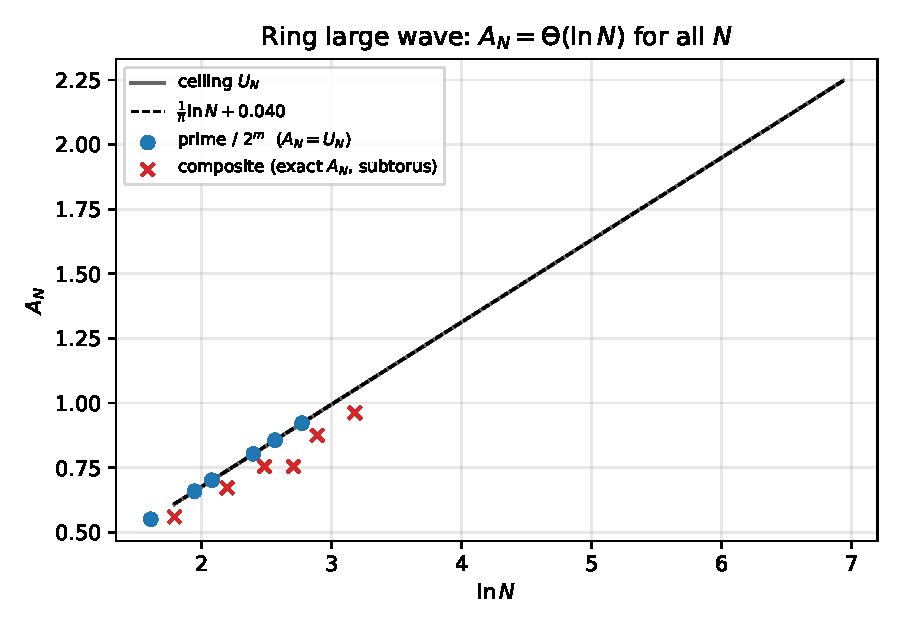
\includegraphics[width=.78\textwidth]{fig_ring.pdf}
\caption{Ring large wave $A_N$ versus $\ln N$. The ceiling $U_N$ (Lemma~\ref{lem:asym}) grows as
$\tfrac1\pi\ln N+0.040$; for primes and $N=2^m$ the supremum equals $U_N$
(Theorems~\ref{thm:prime},~\ref{thm:two}); for composite $N$ the exact subtorus value lies slightly
below, and conjecturally $A_N=\Theta(\ln N)$ for every $N$ (Conjecture~\ref{conj:order}).}\label{fig:ring}
\end{figure}

\subsection{Weyl equidistribution and the lower-bound problem}\label{sub:weyl}
The orbit-closure optimization is rigorous via Weyl's theorem. The frequency vector
$\omega=(\omega_1,\dots,\omega_m)$ defines the linear flow $t\mapsto t\omega\bmod2\pi$, whose closure is
the subtorus
\[
  \mathbb{T}_N=\bigl\{\varphi\in\mathbb{T}^{m}:\langle k,\varphi\rangle\equiv0\ (2\pi)\ \forall k\in\Lambda\bigr\},
  \qquad \Lambda=\{k\in\Z^m:\langle k,\omega\rangle=0\},
\]
of dimension $\dim\mathbb{T}_N=m-\operatorname{rank}\Lambda=\operatorname{rank}_\Q\{\omega_r\}$, the
$\Q$-rank of Section~\ref{sec:prime}. This rank has a closed form, valid for \emph{all} $N$.

\begin{theorem}[subtorus dimension]\label{thm:qrank}
For every $N\ge3$,
\begin{equation}\label{eq:qrank}
  \dim\mathbb{T}_N=\operatorname{rank}_\Q\{2\sin(\tfrac{\pi r}{N}):1\le r\le N-1\}=\tfrac12\varphi(2N).
\end{equation}
\end{theorem}

\begin{proof}
Write $\zeta=\zeta_{2N}$ and let $\sigma:\zeta\mapsto\zeta^{-1}$ be complex conjugation, an involution of
$\Q(\zeta)$ whose fixed field is the maximal real subfield $\Q(\zeta+\zeta^{-1})$, of degree
$\tfrac12\varphi(2N)$. In characteristic $0$, $\Q(\zeta)=V^+\oplus V^-$ where $V^\pm$ are the
$\pm1$-eigenspaces of $\sigma$; thus $\dim_\Q V^\pm=\tfrac12\varphi(2N)$, and since $\sigma$ is the
restriction of conjugation, $V^-$ is exactly the set of purely imaginary elements of $\Q(\zeta)$.
Now $2\mathrm i\sin(\pi r/N)=\zeta^r-\zeta^{-r}=(1-\sigma)\zeta^r$. For any $y$, $\sigma((1-\sigma)y)=
-(1-\sigma)y$, so $(1-\sigma)\Q(\zeta)\subseteq V^-$; and $(1-\sigma)x=2x$ for $x\in V^-$, so the inclusion
is an equality. The powers $\{\zeta^r:r\in\Z\}$ span $\Q(\zeta)$ over $\Q$ (they contain the power basis
$1,\zeta,\dots,\zeta^{\varphi(2N)-1}$), hence their images $\{\zeta^r-\zeta^{-r}\}$ span
$(1-\sigma)\Q(\zeta)=V^-$. Finally $\zeta^N=-1$ gives $\zeta^{N+s}-\zeta^{-(N+s)}=-(\zeta^s-\zeta^{-s})$
while $r=0,N$ give $0$, so the values for $1\le r\le N-1$ already span $V^-$. Dividing by $2\mathrm i$ is a
$\Q$-linear bijection of $V^-\subset\mathrm i\R$ onto $\operatorname{span}_\Q\{\sin(\pi r/N)\}\subset\R$,
which therefore has dimension $\dim_\Q V^-=\tfrac12\varphi(2N)$.
\end{proof}

\noindent The formula is independently confirmed by an exact integer-rank certificate for $N\le64$
(\texttt{verify\_qrank\_formula.py}). Hence full rank---and therefore $A_N=U_N$---holds \emph{exactly}
when $\tfrac12\varphi(2N)=\lfloor N/2\rfloor$, i.e.\ for $N$ prime or $N=2^m$ (Figure~\ref{fig:qrank}):
precisely the scope of Theorems~\ref{thm:prime} and~\ref{thm:two}, now the full-rank case of one
formula. Hence \eqref{eq:subtorus} is \emph{exactly}
\[
  A_N=\max_j\ \max_{\varphi\in\mathbb{T}_N}\frac2N\sum_r\cos\frac{2\pi rj}{N}\,\sin\varphi_r .
\]
For any $S$ with
$\{\omega_r\}_{r\in S}$ $\Q$-independent, the projection of $\mathbb{T}_N$ onto the $S$-coordinates is
the full torus $\mathbb{T}^{|S|}$, so those phases align and contribute $(2/N)\sum_{r\in S}\omega_r^{-1}$;
for the independent low-mode prefix this is the budget $L_{\mathrm{pre}}(N)\gtrsim\tfrac14\ln N$
(Observation~\ref{obs:prefix}). This is \emph{not} yet a lower bound on $A_N$: the out-of-prefix modes
contribute through the relation lattice $\Lambda$ and may interfere destructively, which is the gap to a
proof of Conjecture~\ref{conj:order}.

\smallskip
\noindent\textbf{Open problem.} Prove $A_N\ge c\ln N$ for all $N$ with an absolute constant $c>0$
(equivalently, a sharp lower bound on the subtorus maximum). A certified value for each $N$ is
available from the Lasserre moment--SOS hierarchy; the analytic obstruction is the control of the
rational relations among $\{2\sin(\pi r/N)\}$---a question in the arithmetic of cyclotomic fields.
The evidence is strong on two fronts (Table~\ref{tab:order}): the exact $A_N$ keeps $A_N/\ln N$ in the
narrow band $[0.28,0.34]$ across all classes---including the hardest $N=pq$ with $p,q\sim\sqrt N$, where
in fact $A_N/\ln N\in[0.320,0.322]$ and $A_N/U_N\ge0.98$ for the consecutive-prime products
$N=143,221,323,19\cdot23=437$ (\texttt{verify\_order\_extended.py})---and the $\Q$-independent low-mode
prefix carries a budget $L_{\mathrm{pre}}(N)\gtrsim0.26\ln N$ even for the most composite $N$
(e.g.\ $N=210,330,510$). The gap to a proof is precisely the interference of the out-of-prefix
modes (Observation~\ref{obs:prefix}): aligning the prefix to $\sin=1$ leaves the remaining modes, of total
weight $U_N-L_{\mathrm{pre}}$---a \emph{constant fraction} of $U_N$, not $O(1/N)$---uncontrolled, so
$L_{\mathrm{pre}}$ is a heuristic budget, not a proven lower bound. Only when that residual weight is
$O(1/N)$, as for $N=2p$ (Proposition~\ref{prop:2p}), does the prefix contribution provably survive; the
analogous sub-cycle alignment ($C_p\hookrightarrow C_N$) fails for the same reason. What is missing is the
control of this interference for general $N$.

\begin{table}[ht]\centering
\caption{Evidence for Conjecture~\ref{conj:order}. Left: the exact node-$0$ amplitude keeps $A_N/\ln N$
tightly banded. Right: the $\Q$-independent prefix contributes
$L_{\mathrm{pre}}(N)=\tfrac1N\sum_{r\le M(N)}\csc\tfrac{\pi r}N$, exceeding $0.26\ln N$ even for highly
composite $N$ (a heuristic budget, \emph{not} a proven lower bound on $A_N$---the out-of-prefix modes may
interfere, Observation~\ref{obs:prefix}). $U_N/\ln N\to1/\pi=0.3183$
(\texttt{verify\_conj\_order\_map.py}).}\label{tab:order}
\begin{tabular}{rlcc@{\qquad\qquad}rrc}
\toprule
$N$ & class & $A_N/U_N$ & $A_N/\ln N$ & $N$ & $M(N)$ & $L_{\mathrm{pre}}/\ln N$\\
\midrule
$5$  & prime     & $1.000$ & $0.342$ & $30$  & $8$  & $0.261$\\
$24$ & composite & $0.915$ & $0.303$ & $120$ & $32$ & $0.274$\\
$60$ & composite & $0.873$ & $0.286$ & $210$ & $48$ & $0.268$\\
$64$ & $2^m$     & $1.000$ & $0.328$ & $240$ & $64$ & $0.279$\\
$90$ & composite & $0.875$ & $0.286$ & $300$ & $80$ & $0.281$\\
\bottomrule
\end{tabular}
\end{table}

\begin{figure}[ht]\centering
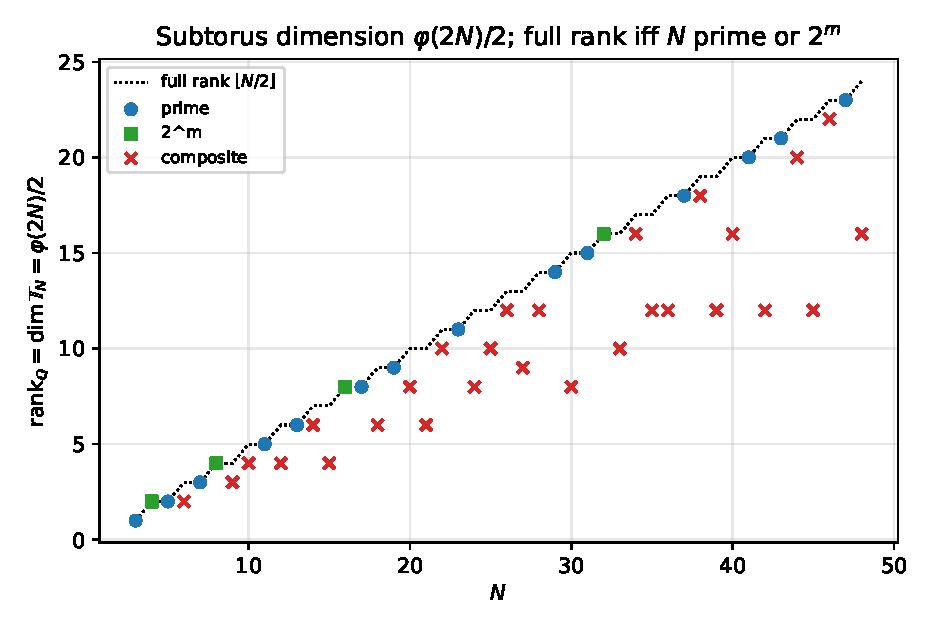
\includegraphics[width=.7\textwidth]{fig_qrank.pdf}
\caption{The subtorus dimension $\tfrac12\varphi(2N)$ \eqref{eq:qrank}. Primes and powers of two attain
the full rank $\lfloor N/2\rfloor$ (dotted), so $A_N=U_N$; composite $N$ fall below (the sub-torus
defect).}\label{fig:qrank}
\end{figure}

\section{Reachability of the ceiling: finite time and disorder}\label{sec:reach}

The supremum $A_N$ is an \emph{infinite-time} quantity. Two refinements bring out its physical content:
how long one must wait, and how fragile the arithmetic that makes the wait short.

\subsection{Finite-time amplification}
Define the finite-horizon amplitude
\[
  A_N(T)=\sup_{0\le t\le T}\,\max_j|u_j(t)|\ \le\ A_N .
\]
Reaching
$(1-\varepsilon)U_N$ requires $\sin(\omega_r t)\approx1$ for all $m=\lfloor N/2\rfloor$ frequencies at
once---a simultaneous Diophantine approximation of the phases to $\tfrac\pi2$. By Dirichlet, such an
alignment to tolerance $\delta$ \emph{exists} by time $\sim\delta^{-m}$---a crude exponential
\emph{upper} bound on the recurrence time
\[
  T_\varepsilon(N)=\inf\{T:A_N(T)\ge(1-\varepsilon)U_N\}.
\]
(This targets $U_N$, so $T_\varepsilon(N)$ is finite only on the saturating classes $N$ prime and $2^m$;
for non-saturating $N$, where $A_N<U_N$, one replaces $U_N$ by $A_N$.) A matching \emph{lower} bound
(that one must wait at least exponentially long) does \emph{not} follow
from Dirichlet, which bounds the wait from above; it would require Diophantine lower bounds on the
badly-approximable phase vector, and is left open. Numerically the wait does grow exponentially: for
primes $\log T_{0.2}(N)$ grows by $\approx0.63$ per unit $N$
(\texttt{verify\_finite\_time.py}, Figure~\ref{fig:reach}), and at a \emph{fixed} horizon $T$ the efficiency $A_N(T)/U_N$
\emph{decreases} with $N$ (from $\approx1.0$ at $N=5$ to $\approx0.70$ at $N=29$ for $T=300$): more
frequencies are harder to align in bounded time. Thus the logarithmic law is an infinite-time ceiling; a physical large wave is the
partial early alignment, already a several-fold over-amplification, while the full $U_N$ is approached
only over astronomically long times. The clean arithmetic of prime and $2^m$ $N$ is what makes a sizable
fraction of $U_N$ reachable \emph{quickly}.

\subsection{Disorder}
Unequal masses $m_j=1+\varepsilon\xi_j$ turn the chain into the generalized problem $\LN v=\omega^2 Mv$,
$M=\operatorname{diag}(m_j)$, with node-$0$ response $x_0(t)=\sum_r c_r\sin(\omega_r t)$,
$c_r=v_r(0)^2/\omega_r>0$ ($M$-orthonormal modes $v_r^\top M v_s=\delta_{rs}$, unit velocity impulse) and
incoherent ceiling $C=\sum_r c_r$. Generic masses destroy every rational relation almost surely (each
relation is a nontrivial real-analytic condition on the masses, and a countable union of such conditions
still has measure zero), so the obstruction of Theorem~\ref{thm:ceiling} disappears and \emph{every} $N$
can in principle reach its ceiling. We verify (\texttt{verify\_disorder.py}) that the exact resonance
residual of a composite $N$ jumps from $0$ to $O(\varepsilon)$ under disorder, and that over a long
horizon the achievable efficiency $A/C$ rises above the blocked ordered value (e.g.\ $N=15$:
$0.83\!\to\!0.91$). But the gain is purely infinite-time: at a short horizon the same disorder yields no
improvement, because the now-independent but near-resonant frequencies need Diophantine time to align.
The dichotomy is sharp: an infinitesimal perturbation makes the absolute ceiling attainable in principle
while pushing the time to attain it beyond any physical horizon. Infinite-time amplification improves;
finite-time amplification does not.

\begin{figure}[ht]\centering
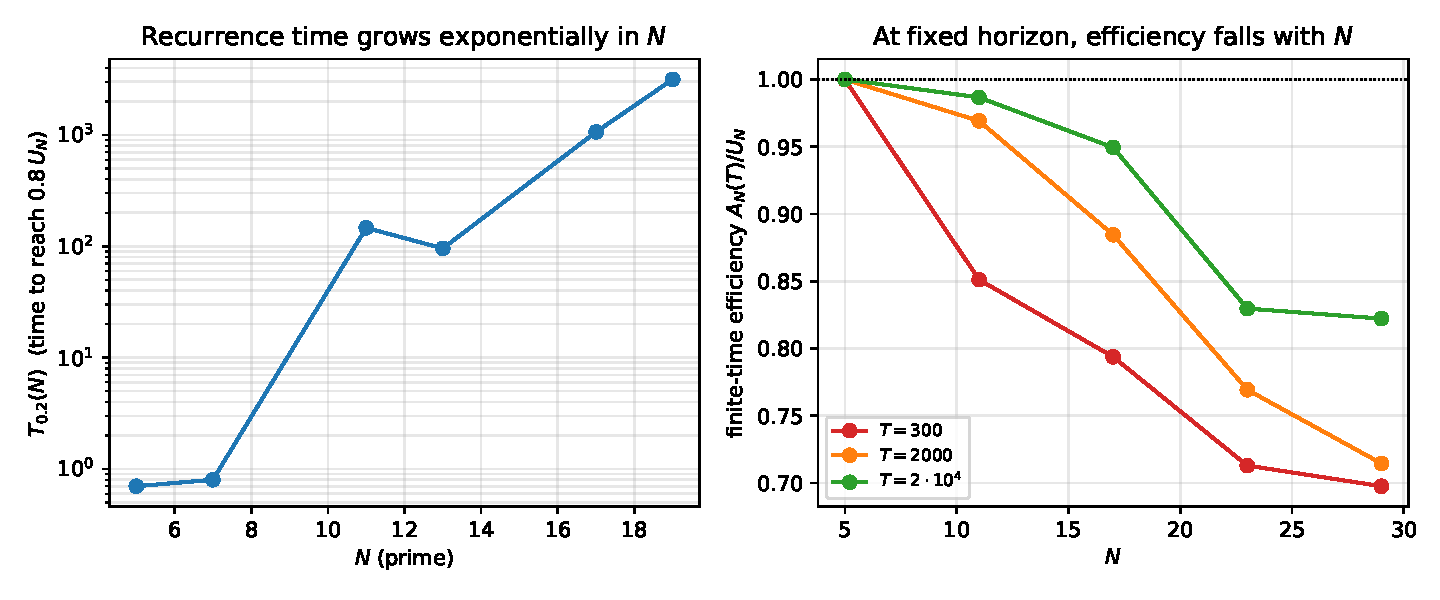
\includegraphics[width=.92\textwidth]{fig_reachability.pdf}
\caption{Reachability of the ceiling. Left: the recurrence time $T_{0.2}(N)$ to reach $0.8\,U_N$ appears to grow
exponentially over the tested prime range (log scale). Right: at a fixed horizon $T$ the finite-time efficiency
$A_N(T)/U_N$ \emph{decreases} with $N$---more frequencies are harder to align in bounded time. The
logarithmic law is an infinite-time ceiling.}\label{fig:reach}
\end{figure}

\section{The discrete Schr\"odinger equation on the ring}\label{sec:schr}

Following Filimonov~\cite{F23}, consider $\mathrm{i}\dot z=\LN z$, so $z(t)=\eu^{-\mathrm{i}t\LN}z(0)$ with kernel
\[
  K_N(k,t)=\frac1N\sum_r\eu^{-\mathrm{i}t\lambda_r}\,\eu^{2\pi\mathrm{i}rk/N}.
\]
Here the phases are governed by $\lambda_r=2-2\cos\tfrac{2\pi r}{N}$, not by $\omega_r=\sqrt{\lambda_r}$.

\begin{theorem}[Schr\"odinger contrast]\label{thm:schr}
\begin{enumerate}
\item (Unitarity.) For $z(0)=e_0$, $\ \max_j|z_j(t)|\le1$ for all $t$: a localized state is never
amplified, in sharp contrast with the bead chain.
\item (Ballistic $\ell^\infty$ amplification.)
$B_N:=\sup_t\|\eu^{-\mathrm{i}t\LN}\|_{\ell^\infty\to\ell^\infty}=\sup_t\sum_k|K_N(k,t)|\le\sqrt N$
(each row of the unitary $\eu^{-\mathrm it\LN}$ has unit $\ell^2$ norm, so $\ell^1$ norm $\le\sqrt N$).
Together with the matching lower bound (Theorem~\ref{thm:schr-lower}), $B_N=\Theta(\sqrt N)$, not $\ln N$.
\item (Arithmetic.) The spectrum lies in the real cyclotomic field $\Q(\zeta_N)^+$ via $\cos$ (whereas
$\{\omega_r\}\subset\Q(\zeta_{2N})$ via $\sin$); the affine identity $\sum_r\lambda_r=2N$ holds always,
and $\rank_\Q\{\lambda_r\}$ is strictly smaller than $\rank_\Q\{\omega_r\}$ for $N=2^m$
(e.g. $4$ vs $8$ at $N=16$).
\end{enumerate}
\end{theorem}

\begin{theorem}[Schr\"odinger lower bound]\label{thm:schr-lower}
$B_N\ge c\sqrt N$ with an absolute constant $c>0$; in fact $\liminf_N B_N/\sqrt N\ge\tfrac12 c_0$ with
$c_0=(2/\pi)^{3/2}B(\tfrac12,\tfrac34)$, i.e.\ $\liminf_N B_N/\sqrt N\ge0.6086$, so for every $c<0.6086$ one has $B_N\ge c\sqrt N$ for all large
$N$ (a finite check of the small cases then gives an absolute $c>0$). With Theorem~\ref{thm:schr}(2),
$B_N=\Theta(\sqrt N)$.
\end{theorem}

\begin{proof}
Evaluate the $\ell^1$ mass at $t=N/8$, so $2t=N/4$. By the Poisson periodization \eqref{eq:poisson},
$K_N(j,N/8)=\sum_{\ell}K_\infty(j+\ell N,N/8)$ with $|K_\infty(n,N/8)|=|J_n(N/4)|$. The Bessel front sits
at $|n|\approx2t=N/4$; beyond it the bound $|J_n(x)|\le(x/2)^{|n|}/|n|!$ (valid for all $n\ge0$) forces
super-exponential decay for $|n|>N/4$, so the aliasing copies $\ell\ne0$, supported at
$|j+\ell N|\ge N/2$, contribute an exponentially small amount. Hence
$\sum_{j}|K_N(j,N/8)|=(1+o(1))\sum_{n\in\Z}|J_n(N/4)|$. The classical $\ell^1$ Bessel asymptotics
$\sum_{n}|J_n(x)|\sim c_0\sqrt x$, $c_0=(2/\pi)^{3/2}B(\tfrac12,\tfrac34)\approx1.217$ (the envelope
$|J_n(x)|\approx\sqrt{2/(\pi\sqrt{x^2-n^2})}$ integrated against $\langle|\cos|\rangle=2/\pi$), give
$\sum_n|J_n(N/4)|\sim c_0\sqrt{N/4}=\tfrac12 c_0\sqrt N$ with $\tfrac12 c_0\approx0.6086$. Therefore
$\liminf_N B_N/\sqrt N\ge\lim_N\sum_j|K_N(j,N/8)|/\sqrt N=\tfrac12 c_0$, so for every $c<\tfrac12 c_0$ one
has $B_N\ge c\sqrt N$ for all large $N$, and a finite scan of the small cases supplies an absolute $c>0$
(the finite-$N$ values decrease to $\tfrac12 c_0$ from above, Table~\ref{tab:bn}); the upper bound is
Theorem~\ref{thm:schr}(2).
\end{proof}

\noindent Part (1) is unitarity of $\eu^{-\mathrm{i}t\LN}$; the bounds in (2) are now both rigorous
(upper from unitarity, lower from Theorem~\ref{thm:schr-lower}), and every step of the proof---the
periodization, the negligible aliasing at $t=N/8$, the $\sqrt N$ growth with constant
$\tfrac12 c_0\approx0.6086$, and the $c_0\sqrt x$ Bessel asymptotics---is reproduced numerically (\texttt{verify\_schrodinger\_lower.py},
\texttt{verify\_theorem3\_schrodinger.py}, \texttt{verify\_bessel\_kernel.py}). The constant itself is
mapped in Table~\ref{tab:bn}.

\begin{table}[ht]\centering
\caption{The constant in $B_N=\Theta(\sqrt N)$. A refined $t$-scan (uniform grid $+$ structured candidate times
$t=\pi a/N$) gives $B_N/\sqrt N$; the proven Bessel point $t=N/8$ gives the lower row. The largest value in the
finite scan, $\approx0.96$, lies inside the rigorous band $[\tfrac12 c_0,1]\approx[0.6086,1]$, and the
exact limit is open
(\texttt{verify\_bn\_constant.py}).}\label{tab:bn}
\begin{tabular}{lcccccc}
\toprule
$N$ & $16$ & $64$ & $256$ & $512$ & $1024$ & $2048$\\
\midrule
$B_N/\sqrt N$ (scan)            & $0.960$ & $0.907$ & $0.888$ & $0.880$ & $0.875$ & $0.870$\\
$\|K_N(\cdot,N/8)\|_1/\sqrt N$  & $0.770$ & $0.694$ & $0.658$ & $0.637$ & $0.634$ & $0.626$\\
\bottomrule
\end{tabular}
\end{table}

\subsection{Bessel kernel and Poisson summation}
On the infinite chain $\Z$ the propagator kernel follows from the symbol by a contour integral,
\begin{equation}\label{eq:bessel}
  K_\infty(n,t)=\frac1{2\pi}\int_{-\pi}^{\pi}\eu^{\mathrm in\theta}\,\eu^{-\mathrm it(2-2\cos\theta)}\,d\theta
  =\eu^{-2\mathrm it}\,\mathrm i^{\,n}J_n(2t),
\end{equation}
by the Jacobi--Anger identity $\frac1{2\pi}\int\eu^{\mathrm i(n\theta+x\cos\theta)}\,d\theta=\mathrm i^nJ_n(x)$~\cite{Watson}.
Thus $|K_\infty(n,t)|=|J_n(2t)|$: a ballistic light cone $|n|\approx2t$ with an Airy front of height
$\max_n|J_n(2t)|\sim0.6748\,(2t)^{-1/3}$ (Figure~\ref{fig:bessel}). Unitarity gives $\sum_n|K_\infty|^2=1$,
while the $\ell^1$ mass $\sum_n|J_n(2t)|\sim c\sqrt t$ grows---the infinite-chain shadow of
$B_N\sim\sqrt N$. The ring kernel is the Poisson periodization
\begin{equation}\label{eq:poisson}
  K_N(j,t)=\sum_{\ell\in\Z}K_\infty(j+\ell N,t),
\end{equation}
verified to machine precision; the large wave survives only through this finite-$N$ folding, since on
$\Z$ the front escapes and the peak decays.

\begin{figure}[ht]\centering
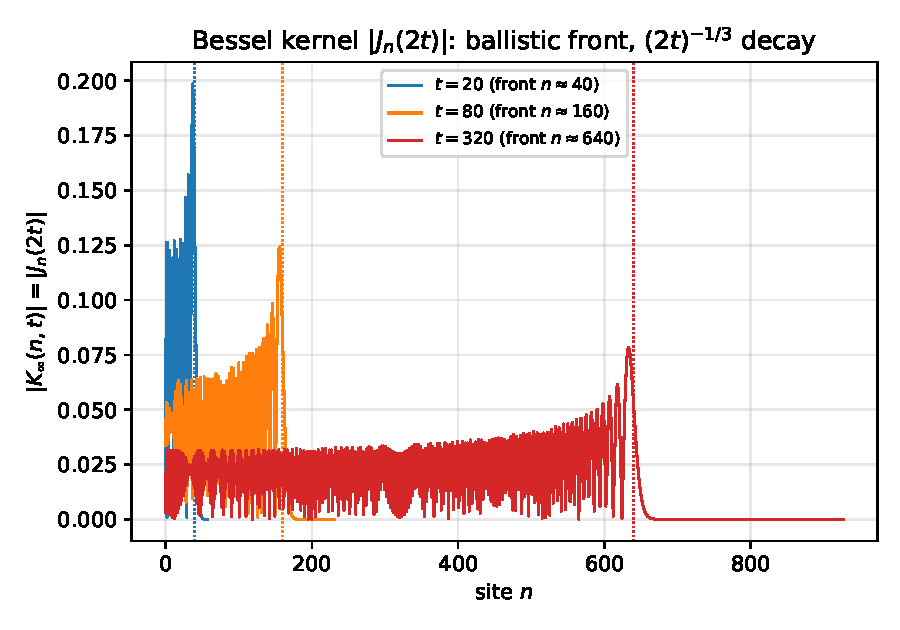
\includegraphics[width=.74\textwidth]{fig_bessel.pdf}
\caption{Infinite-chain Schr\"odinger kernel $|K_\infty(n,t)|=|J_n(2t)|$: a ballistic front at
$n\approx2t$ (dotted) whose height decays as $(2t)^{-1/3}$. On the ring this kernel is periodized,
\eqref{eq:poisson}; the effect is intrinsically finite-size.}\label{fig:bessel}
\end{figure}

\subsection{Arithmetic dynamics: revivals and Gauss sums}
The recurrence structure of $\eu^{-\mathrm i t\LN}$ is arithmetic. Since $2\cos(2\pi/N)$ is rational
only for $N\in\{1,2,3,4,6\}$ (Niven's theorem~\cite{Niven}; for general $r$, $2\cos(2\pi r/N)$ is
rational only when $r/N$ reduces to such a denominator), the tight-binding spectrum is generically
incommensurate: $\eu^{-\mathrm i t\LN}$ has \emph{no finite revival period}, and the return amplitude
$|K_N(0,t)|$ is almost-periodic, approaching $1$ along a wandering sequence of near-revival times
(\texttt{verify\_revivals\_gauss.py}). In the long-wave limit $\lambda_r\approx(2\pi r/N)^2$ the model
approaches the \emph{quadratic} dispersion of a free particle, where the dynamics becomes exactly
arithmetic: at the Talbot times $t=2\pi s/q$ (in the rescaled time $\tau=(2\pi/N)^2 t$ of this quadratic
limit) the propagator kernel is a quadratic Gauss sum, and for
odd $q$ with $\gcd(a,q)=1$,
\[
  \Bigl|\sum_{n=0}^{q-1}\eu^{2\pi\mathrm i a n^2/q}\Bigr|=\sqrt q,
\]
yielding an exact fractional revival of uniform amplitude $|U_{jk}|=1/\sqrt q$ (and a full revival
$U(2\pi)=I$). The large wave thus inhabits the almost-periodic, Diophantine regime of the lattice, of
which the discrete Talbot effect and Gauss-sum revivals are the exactly solvable continuum shadow.

\begin{figure}[ht]\centering
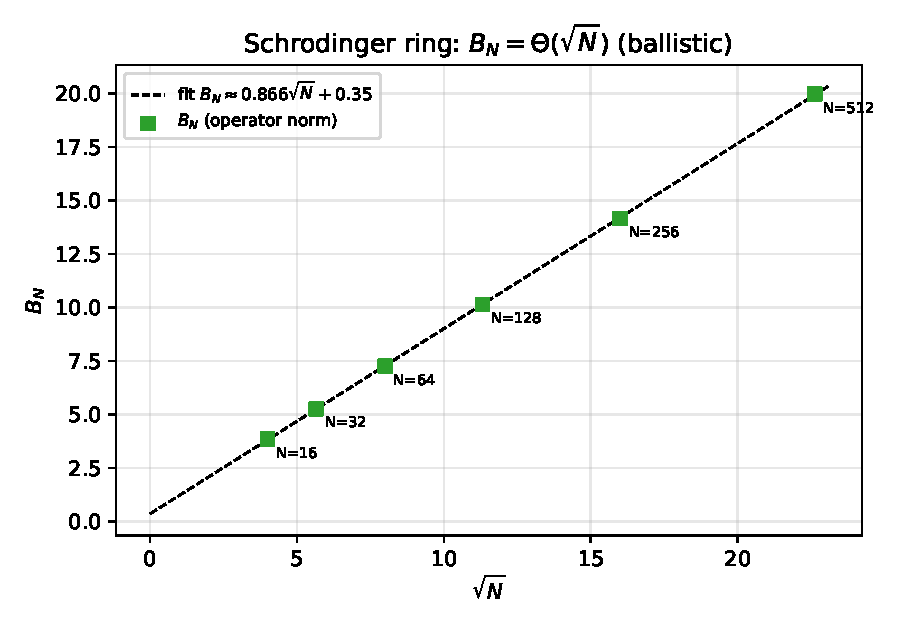
\includegraphics[width=.78\textwidth]{fig_schrodinger.pdf}
\caption{Discrete Schr\"odinger propagator: the $\ell^\infty\!\to\!\ell^\infty$ amplification
$B_N$ grows ballistically as $\Theta(\sqrt N)$ (linear fit in $\sqrt N$, $R^2=1.0000$), unlike the
$\ln N$ growth of the bead chain.}\label{fig:schr}
\end{figure}

\subsection{Dirichlet segment: a logarithmic site-amplitude law}\label{sub:filimonov}
The sharpest large-wave statement for the discrete Schr\"odinger equation is Filimonov's~\cite{F23}, and
it lives on the \emph{open} (Dirichlet) chain rather than the ring. With on-site value
$\varepsilon_j\equiv-2$ and pinned ends $z_0=z_N=0$,
\[
  \mathrm i\dot z_j=z_{j+1}-2z_j+z_{j-1},\qquad z_j(0)=\alpha_j,\qquad 1\le j\le N-1,
\]
the Dirichlet sine basis diagonalizes the flow and the solution is explicit,
\begin{equation}\label{eq:fil-sol}
  z_j(t)=\eu^{2\mathrm it}\sum_{k=1}^{N-1}a_k\sin\frac{\pi kj}{N}\,\eu^{-2\mathrm i\omega_k t},
  \qquad \omega_k=\cos\frac{\pi k}{N},\qquad a_k=\frac2N\sum_{r=1}^{N-1}\alpha_r\sin\frac{\pi kr}{N}.
\end{equation}
The simple spectrum $\{\omega_k=\cos(\pi k/N)\}$ replaces the twofold-degenerate ring frequencies. For the
uniform initial state $\alpha_j\equiv1$ the coefficient sum is the imaginary part of a geometric series,
$\sum_{r=1}^{N-1}\sin(\pi kr/N)=\cot(\pi k/2N)$ for odd $k$ and $0$ for even $k$, so
\begin{equation}\label{eq:fil-ak}
  a_k=\frac2N\cot\frac{\pi k}{2N}\ \ (k\ \text{odd}),\qquad a_k=0\ \ (k\ \text{even}).
\end{equation}
The pointwise ceiling is $d_j^N:=\sum_{k=1}^{N-1}\bigl|a_k\sin(\pi kj/N)\bigr|$, with $|z_j(t)|\le d_j^N$
for all $t$ by the triangle inequality.

\begin{theorem}[Filimonov~\cite{F23}]\label{thm:filimonov}
For $\alpha_j\equiv1$ and $N=2^m$, $\ \sup_t|z_j(t)|=d_j^N$, and
\begin{equation}\label{eq:fil-lnj}
  \lim_{N\to\infty}d_j^N=C\ln j+O(1).
\end{equation}
\end{theorem}

\noindent Thus the Schr\"odinger amplitude at the \emph{observation site} $j$ grows without bound
(logarithmically) as $j\to\infty$---a large wave at the far end of the chain, attained along the
relatively dense set of near-revival times (the modulus is almost-periodic, \cite{Bohr}). Two refinements
complete the picture (\texttt{verify\_filimonov\_schrodinger.py}).

\emph{The constant.} Filimonov leaves $C$ unspecified; we identify it. As $N\to\infty$ the ceiling
\eqref{eq:fil-ak} becomes a Riemann sum for
\begin{equation}\label{eq:fil-int}
  d_j^\infty=\frac2\pi\int_0^{\pi/2}\cot\theta\,\bigl|\sin 2j\theta\bigr|\,d\theta,
\end{equation}
and since $\cot\theta\sim\theta^{-1}$ near $0$ while $\langle|\sin|\rangle=2/\pi$, the integral grows like
$\tfrac2\pi\cdot\tfrac2\pi\ln j$, giving
\begin{equation}\label{eq:fil-C}
  C=\frac{4}{\pi^2}\approx0.4053 .
\end{equation}
The fit $d_j^N=(4/\pi^2)\ln j+O(1)$ holds to $R^2=1.0000$ at $N=2^{12}$ (Figure~\ref{fig:filimonov}).

\emph{Independence and the scope of Theorem~\ref{thm:filimonov}.} The equality $\sup_t|z_j|=d_j^N$ rests
on two facts: the sign-pairing $\omega_{N-k}=-\omega_k$ together with the elementary identity
$\max(|x+y|,|x-y|)=|x|+|y|$ lets each pair reach $|a_k|+|a_{N-k}|$, and the distinct $|\omega_k|$ must be
$\Q$-independent so that all pairs align simultaneously (Kronecker). This independence---the cosine
analogue of Theorems~\ref{thm:prime}--\ref{thm:two}, via $2\cos(\pi k/N)=\zeta_{2N}^k+\zeta_{2N}^{-k}$ in
the \emph{plus}-eigenspace---has full rank $\lfloor(N-1)/2\rfloor$ exactly for $N$ prime or $N=2^m$
(\texttt{verify\_filimonov\_schrodinger.py}), which \emph{suffices} for $\sup_t|z_j|=d_j^N$ at every site
$j$; so Filimonov's $N=2^m$ extends to prime $N$. Full rank is not \emph{necessary}, however: composite
$N$ can still saturate at individual sites---numerically $\sup_t|z_j|=d_j^N$ already at $j=1$ for
$N=6,9,10,12$, the alignment there needing only the active frequencies and the sign-pairing---so a
complete classification of composite saturation is open.

\emph{Three laws on one Laplacian.} The discrete Laplacian thus carries several distinct large-wave
asymptotics, one per dynamics and functional (Table~\ref{tab:laws}): $A_N\sim\tfrac1\pi\ln N$ (ring,
growth in the system size $N$), $B_N\sim\sqrt N$ (ring, $\ell^\infty\!\to\!\ell^\infty$ operator norm),
and $d_j^N\sim\tfrac4{\pi^2}\ln j$ (Dirichlet segment, growth in the observation site $j$).

\begin{table}[ht]\centering
\caption{The large-wave asymptotics carried by the discrete Laplacian, by dynamics and functional; every
constant is reproduced by the accompanying scripts. ``Sharp class'' is where the leading constant is
established (proved or, for $d_j^N$, identified here).}\label{tab:laws}
\begin{tabular}{llll}
\toprule
quantity & dynamics / functional & leading asymptotic & sharp class\\
\midrule
$U_N$ & ring, velocity ceiling & $\tfrac1\pi\ln N+\tfrac1\pi(\gamma+\ln\tfrac2\pi)$ & all $N$\\
$A_N$ & ring, $\sup_t\max_j|G_N(j,\cdot)|$ & $\tfrac1\pi\ln N$ & prime, $2^m$, $2p$\\
$B_N$ & ring, $\ell^\infty\!\to\!\ell^\infty$ Schr\"odinger & $\Theta(\sqrt N)$, const $\in[0.6086,1]$ & all $N$\\
$d_j^N$ & segment, $\sup_t|z_j(\cdot)|$ Schr\"odinger & $\tfrac4{\pi^2}\ln j$ & prime, $2^m$ (suff.)\\
$U_N^{(d)}$ & $d$-torus, velocity ceiling & $\tfrac1\pi\ln N$ ($d{=}1$), $\ O(1)$ ($d{\ge}2$) & $d_s=1$\\
\bottomrule
\end{tabular}
\end{table}

\begin{figure}[ht]\centering
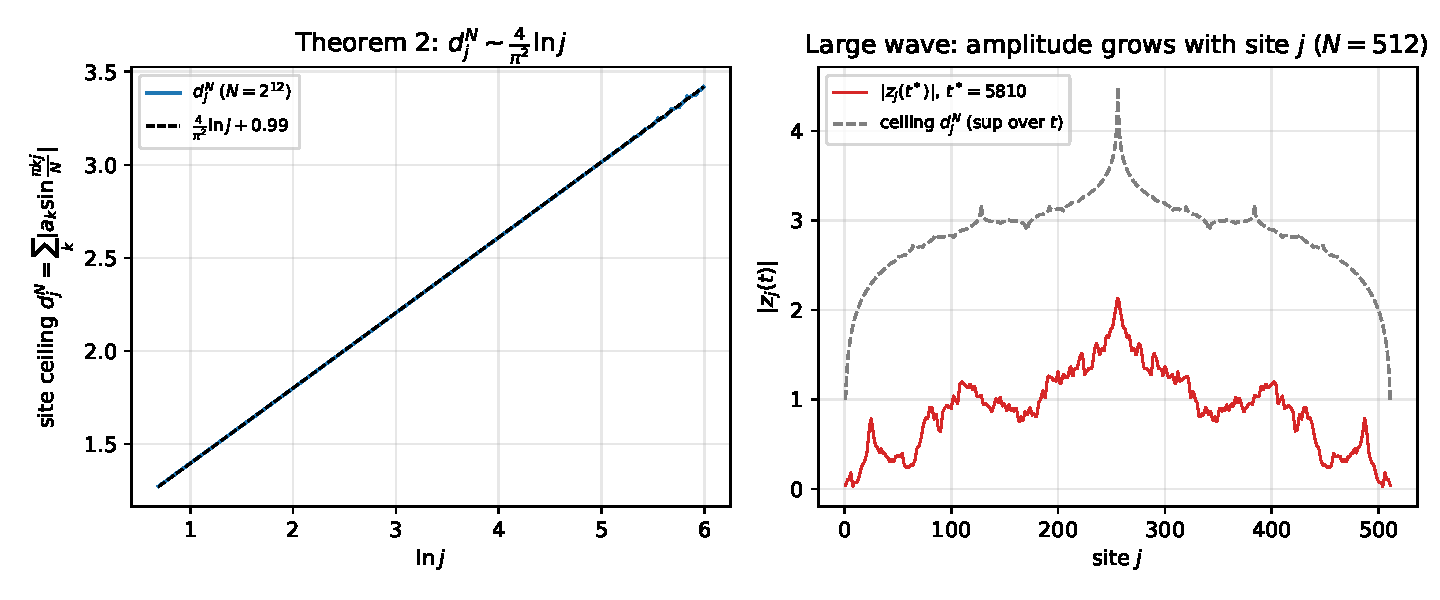
\includegraphics[width=.92\textwidth]{fig_filimonov.pdf}
\caption{Filimonov's segment Schr\"odinger large wave (\texttt{verify\_filimonov\_schrodinger.py}). Left:
the site ceiling $d_j^N$ versus $\ln j$ ($N=2^{12}$) on the line $\tfrac4{\pi^2}\ln j+O(1)$. Right: a
snapshot $|z_j(t^*)|$ at a near-revival time grows with the site $j$ toward the ceiling $d_j^N$
($N=512$).}\label{fig:filimonov}
\end{figure}

\section{Continuum analogue and the step initial condition}

Expanding the symbol for small wavenumbers, $\omega(\theta)=2\sin(\theta/2)=\theta-\theta^3/24+O(\theta^5)$,
recovers to leading order the continuum wave equation $u_{tt}=u_{xx}$ ($\omega=\theta$). A finite Taylor
truncation improves the long-wave fit but diverges from the exact branch near the band edge
$\theta=\pi$. The \emph{two-point Pad\'e} approximant of Andrianov--Awrejcewicz~\cite{AAW}, obtained from the
regularized model $m(1-a^2h^2\partial_x^2)u_{tt}=ch^2u_{xx}$ with $a^2=\tfrac14-\pi^{-2}\approx0.1487$,
yields
\begin{equation}\label{eq:pade}
  \omega_{\mathrm{Pad\acute{e}}}(\theta)=\frac{\theta}{\sqrt{1+a^2\theta^2}},
\end{equation}
which matches the exact dispersion at \emph{both} ends---unit slope at $\theta=0$ and
$\omega=2$ at $\theta=\pi$ (indeed $\pi/\sqrt{1+a^2\pi^2}=2$)---with error below $3\%$ in between
(Figure~\ref{fig:dispersion}). Nonetheless no continuum surrogate reproduces the large wave: as
Section~\ref{sec:schr} shows through the decaying Bessel kernel, the effect is \emph{absent} in the
continuum/infinite limit---it is intrinsically a finite-size, discrete phenomenon driven by the exact
arithmetic of the sampled frequencies $\{2\sin(\pi r/N)\}$.

\begin{figure}[ht]\centering
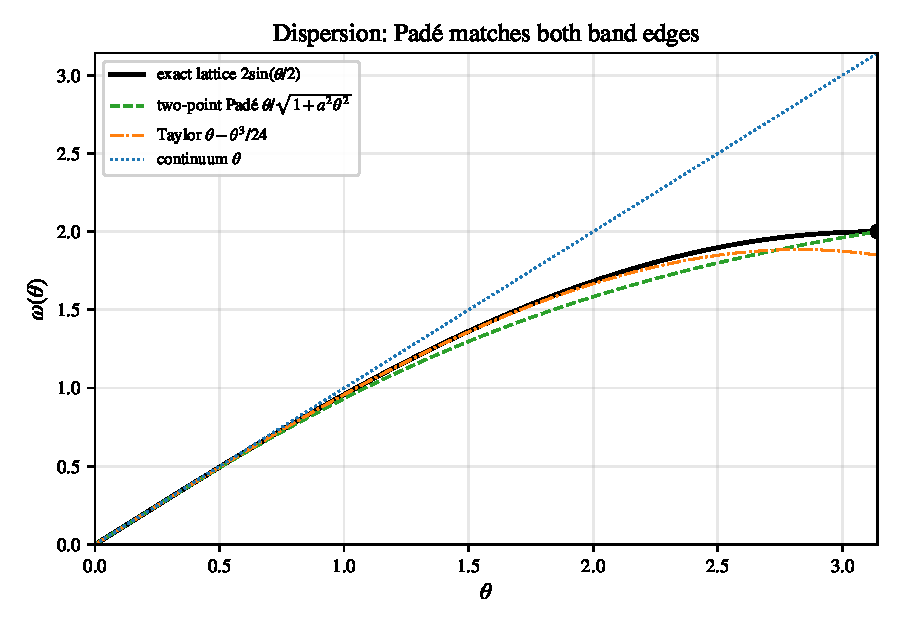
\includegraphics[width=.72\textwidth]{fig_dispersion.pdf}
\caption{Dispersion relations. The exact lattice branch $2\sin(\theta/2)$ is matched at both ends by
the two-point Pad\'e \eqref{eq:pade}, whereas the continuum $\theta$ and the Taylor truncation
$\theta-\theta^3/24$ diverge at the band edge $\theta=\pi$ ($\bullet$, $\omega=2$).}\label{fig:dispersion}
\end{figure}

For the step displacement $u_j(0)=1$ ($1\le j\le N-1$), $u_0(0)=0$, $\dot u(0)=0$, the exact supremum
is, by Bohr's theorem (for $N=2^m$), $\sup_t\max_j u_j(t)=\bar\alpha+\max_j\sum_r|A_{r,j}|\approx2$ for
all $N$, where $\bar\alpha=(N-1)/N$ and $A_{r,j}$ are the modal amplitudes. Earlier numerical work
reported peaks $1.617\to1.397$ for $N=32,\dots,1024$; these are finite-time scan values, and their
\emph{decrease} with $N$ is the expected worsening of the scan undershoot for an almost-periodic
supremum (the true maximum is only approached, at near-recurrence times). The present analysis thus
reproduces the effect and corrects the value to $\approx2$ (\texttt{verify\_thesis\_peaks.py}).

\section{Numerical experiments}\label{sec:experiments}

Table~\ref{tab:experiments} reports both dynamics over the three families $N=2^m$, prime, composite.
The wave $A_N$ is the orbit-closure value of Section~\ref{sec:exact} (exact reduction, evaluated
numerically); it equals the ceiling
$U_N$ for prime and $2^m$ (Theorems~\ref{thm:prime},~\ref{thm:two}) and sits modestly below for
composite $N$. The Schr\"odinger $B_N/\sqrt N$ stays $O(1)$ across all families. Figures~\ref{fig:ring}
and~\ref{fig:schr} display the two growth laws---$\ln N$ for the wave, $\sqrt N$ for Schr\"odinger.

\begin{table}[ht]\centering
\begin{tabular}{llrrrr}
\toprule
family & $N$ & $U_N$ & $A_N$ (wave) & $A_N/U_N$ & $B_N/\sqrt N$ \\
\midrule
$2^m$      & 16 & 0.922 & 0.922 & 1.000 & 0.960 \\
           & 32 & 1.143 & 1.143 & 1.000 & 0.931 \\
           & 64 & 1.364 & 1.364 & 1.000 & 0.906 \\
prime      & 17 & 0.942 & 0.942 & 1.000 & 0.988 \\
           & 31 & 1.133 & 1.133 & 1.000 & 0.971 \\
           & 61 & 1.349 & 1.349 & 1.000 & 0.961 \\
composite  & 12 & 0.831 & 0.755 & 0.908 & 0.971 \\
           & 15 & 0.902 & 0.754 & 0.836 & 0.984 \\
           & 24 & 1.052 & 0.962 & 0.915 & 0.941 \\
\bottomrule
\end{tabular}
\caption{Both dynamics over the three families. Wave $A_N$ (exact, Section~\ref{sec:exact}) equals the
Bohr ceiling $U_N\sim\frac1\pi\ln N$ for prime/$2^m$ and is slightly smaller for composite $N$;
the Schr\"odinger amplification has $B_N/\sqrt N=O(1)$, i.e.\ $B_N=\Theta(\sqrt N)$
(\texttt{verify\_experiments.py}).}\label{tab:experiments}
\end{table}

\begin{figure}[ht]\centering
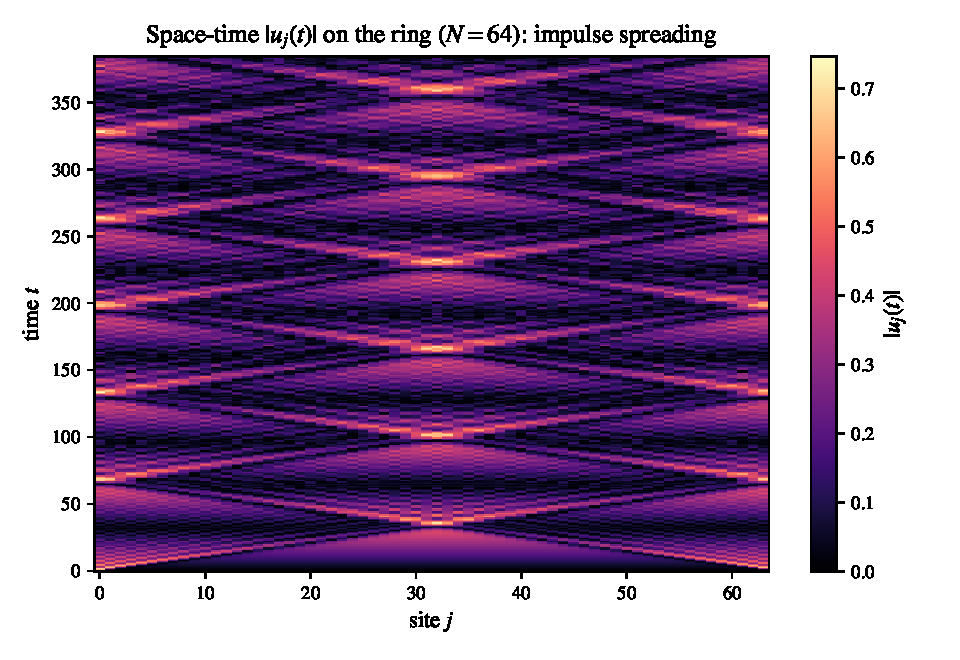
\includegraphics[width=.72\textwidth]{fig_heatmap.pdf}
\caption{Space-time $|u_j(t)|$ for the unit impulse on the $N=64$ ring: ballistic light cones,
reflections off the periodic geometry, and the focusing recurrences that build the large wave.}
\label{fig:heatmap}
\end{figure}

\section{Reproducibility}\label{sec:repro}

Every claim above is reproduced by a standalone script (run via \texttt{uv run --script}); all pass.
\begin{longtable}{ll}
\hline
Claim & Script \\
\hline
\endhead
\hline
\endfoot
Variational ceiling $\sqrt N$, focusing & \texttt{verify\_theorem1.py}\\
Bohr ceiling $A_N=U_N\sim\frac1\pi\ln N$ & \texttt{verify\_bohr\_lower\_bound.py}\\
Independence, $N=p$ (exact rank) & \texttt{verify\_lemma1\_prime.py}\\
$\Q$-rank map (prime/$2^m$/composite) & \texttt{verify\_independence\_rank.py}\\
Lebesgue constant, Bessel decay & \texttt{verify\_lemma3\_lebesgue.py}\\
Prefix budget for all $N$ & \texttt{verify\_lemma4\_prefix.py}\\
Exact $A_N$ via subtorus & \texttt{verify\_exact\_AN.py}\\
Closed form $N=6$, relation $N=12$ & \texttt{verify\_AN\_closed\_form.py}\\
Segment vs ring degeneracy & \texttt{verify\_segment\_vs\_ring.py}\\
Schr\"odinger contrast & \texttt{verify\_theorem3\_schrodinger.py}\\
Step-IC peak vs 2015 scan & \texttt{verify\_thesis\_peaks.py}\\
Bessel kernel \& Poisson summation & \texttt{verify\_bessel\_kernel.py}\\
Consolidated experiments table & \texttt{verify\_experiments.py}\\
Spectral zeta special values & \texttt{verify\_spectral\_zeta.py}\\
Operator-norm hierarchy & \texttt{verify\_operator\_norms.py}\\
Revivals \& Gauss sums & \texttt{verify\_revivals\_gauss.py}\\
Spanning trees / spectral det.\ & \texttt{verify\_spanning\_trees.py}\\
Q-rank formula $\varphi(2N)/2$ & \texttt{verify\_qrank\_formula.py}\\
Statistics (arcsine, Bohr--Jessen) & \texttt{verify\_statistics.py}\\
Rogue waves / DNLS (Peregrine, MI) & \texttt{verify\_rogue\_dnls.py}\\
Dirichlet segment, full-rank class & \texttt{verify\_segment\_lower\_bound.py}\\
Higher-dim tori ($d{=}1,2,3$) & \texttt{verify\_torus\_dimension.py}\\
Asymptotic correction $-\pi/72N^{-2}$ & \texttt{verify\_asymptotic\_corrections.py}\\
Certified composite gap (SOS) & \texttt{verify\_sos\_certified.py}\\
Sharp constant for $N=2p$ & \texttt{verify\_2p\_family.py}\\
Open-problem evidence (defect, $B_N$) & \texttt{verify\_open\_problems.py}\\
DNLS self-trapping / breather & \texttt{verify\_dnls\_selftrapping.py}\\
FPUT-$\beta$ recurrence (symplectic) & \texttt{verify\_fput\_recurrence.py}\\
Lyapunov exponent, route to chaos & \texttt{verify\_lyapunov.py}\\
2D DNLS breather (self-trapping) & \texttt{verify\_dnls\_2d.py}\\
Front $=$ Airy fold caustic ($t^{-1/3}$) & \texttt{verify\_caustic\_airy.py}\\
Branched flow, caustic hot spots & \texttt{verify\_branched\_flow.py}\\
Ray tracing, caustic (geom.\ optics) & \texttt{verify\_ray\_caustic.py}\\
Cusp / Pearcey / teacup nephroid & \texttt{verify\_cusp\_pearcey.py}\\
Caustic seeds self-focusing (lens+NLS) & \texttt{verify\_caustic\_mi.py}\\
Lightning (dielectric breakdown growth) & \texttt{verify\_laplacian\_lightning.py}\\
Ceiling criterion (mod $4$) & \texttt{verify\_ceiling\_criterion.py}\\
Relation lattices $\Lambda_N$ (Table~\ref{tab:lattices}) & \texttt{verify\_relation\_lattices.py}\\
Schr\"odinger lower bound $\Omega(\sqrt N)$ & \texttt{verify\_schrodinger\_lower.py}\\
Constant $B_N/\sqrt N$ scan (Table~\ref{tab:bn}) & \texttt{verify\_bn\_constant.py}\\
Spectral-dimension threshold $d_s{=}1$ & \texttt{verify\_spectral\_dimension.py}\\
Finite-time recurrence $T_\varepsilon(N)$ & \texttt{verify\_finite\_time.py}\\
Disorder vs.\ resonance (gen.\ eig.) & \texttt{verify\_disorder.py}\\
Order map $A_N/\ln N$, prefix (Table~\ref{tab:order}) & \texttt{verify\_conj\_order\_map.py}\\
Extended order run ($N\!\sim\!1000$, criterion $\le500$) & \texttt{verify\_order\_extended.py}\\
Filimonov segment law $d_j^N\!\sim\!\tfrac4{\pi^2}\ln j$ & \texttt{verify\_filimonov\_schrodinger.py}\\
\end{longtable}

\section{Statistics: density of states and value distribution}\label{sec:stats}

The spectrum and the large wave both admit clean probabilistic descriptions, verified in
\texttt{verify\_statistics.py}.

\emph{Density of states.} As $N\to\infty$ the eigenvalues $\lambda_r=4\sin^2(\pi r/N)$---the pushforward
of the uniform law by $\lambda(x)=2-2\cos2\pi x$---converge to the \textbf{arcsine law} on $[0,4]$,
\begin{equation}\label{eq:arcsine}
  \rho(\lambda)=\frac1{\pi\sqrt{\lambda(4-\lambda)}},\qquad F(\lambda)=\frac2\pi\arcsin\frac{\sqrt\lambda}{2}.
\end{equation}
This is the change of variables: $\tfrac{d\lambda}{dx}=4\pi\sin2\pi x=2\pi\sqrt{\lambda(4-\lambda)}$ (since
$\sin2\pi x=\tfrac12\sqrt{\lambda(4-\lambda)}$), and each $\lambda\in(0,4)$ has \emph{two} preimages in
$[0,1]$, so $\rho(\lambda)=2/(d\lambda/dx)=1/(\pi\sqrt{\lambda(4-\lambda)})$---the classical density of
states of the one-dimensional discrete Laplacian (Figure~\ref{fig:dos}); the frequencies have
$\rho(\omega)=2/(\pi\sqrt{4-\omega^2})$ on $[0,2]$. Both fit to Kolmogorov--Smirnov distance $O(N^{-1})$
(a deterministic quantile grid: the empirical CDF lies within $2/N$ of the limit, the $1/N$ jump floor).

\emph{Value distribution.} For prime $N$ the impulse response $u_0(t)$ is almost-periodic with
$\Q$-independent frequencies, so by the Bohr--Jessen theorem its values possess a limiting distribution
(Figure~\ref{fig:dos}, right): symmetric, mean $0$, and variance $\mathrm{Var}_t\,u_0=\tfrac{N^2-1}{12N^2}\to\tfrac1{12}$.
The variance is exact: with $u_0(t)=\tfrac1N\sum_r\omega_r^{-1}\sin(\omega_r t)$ and the time-average
$\langle\sin(\omega_r t)\sin(\omega_s t)\rangle=\tfrac12$ when $\omega_s=\omega_r$ (i.e.\ $s\in\{r,N-r\}$)
and $0$ otherwise, the degeneracy makes each cross-term reinforce the diagonal, so
$\langle u_0^2\rangle=\tfrac1{N^2}\sum_{r}\omega_r^{-2}=\zeta_{\LN}(1)/N^2=\tfrac{N^2-1}{12N^2}$. The law is
\emph{platykurtic} (kurtosis $\approx2.4<3$) because the lowest mode dominates
(weight $1/\omega_1\sim N$, a single arcsine sinusoid). The large wave is therefore \emph{not} a heavy
tail of the typical value but the rare near-alignment supremum (Figure~\ref{fig:largewave}): a spike that
climbs to nearly $U_N$ standing far above the thin-tailed bulk of size $\mathrm{RMS}\approx1/\sqrt{12}$,
$A_N\sim\tfrac1\pi\ln N$.

\begin{figure}[ht]\centering
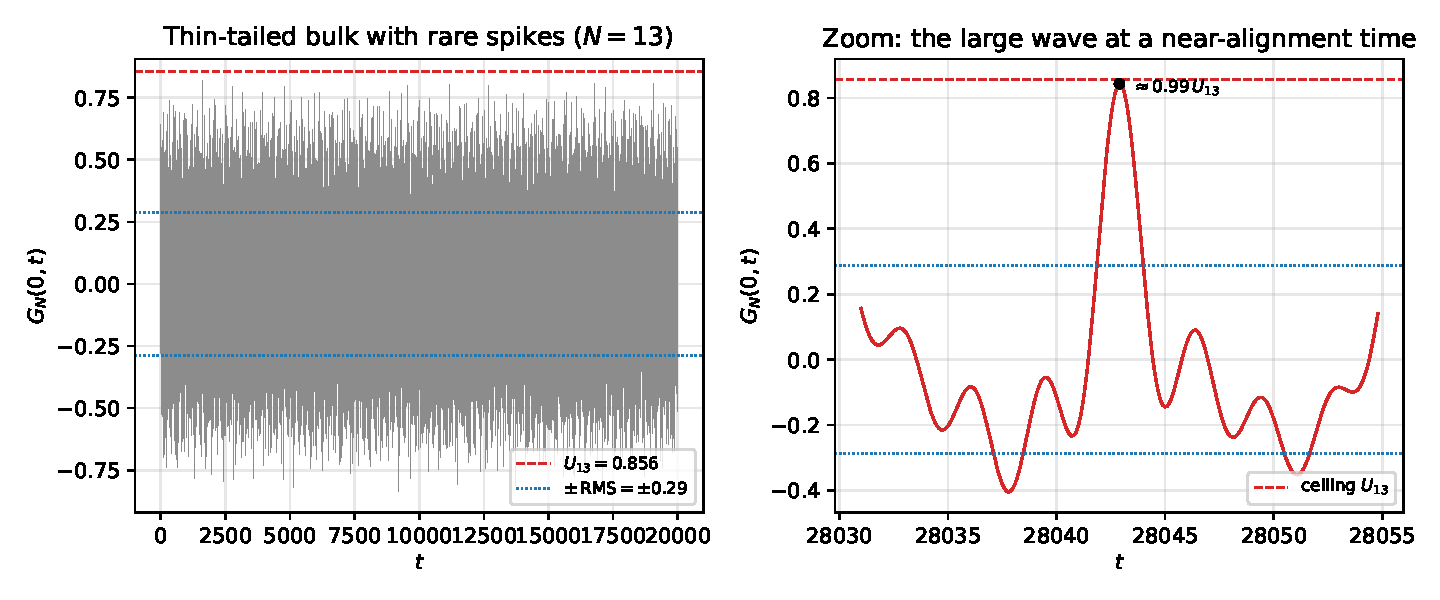
\includegraphics[width=.92\textwidth]{fig_largewave.pdf}
\caption{What the large wave looks like in time ($N=13$, prime). Left: the node-$0$ response $G_N(0,t)$
oscillates within the thin band $\pm\mathrm{RMS}$ ($\mathrm{RMS}\approx0.29$) but throws rare spikes
toward the ceiling $U_{13}=0.856$. Right: a zoom on the largest near-alignment spike, reaching
$\approx0.99\,U_N$---the large wave forming as the modal phases briefly align
(\texttt{verify\_thesis\_peaks.py}).}\label{fig:largewave}
\end{figure}

\begin{figure}[ht]\centering
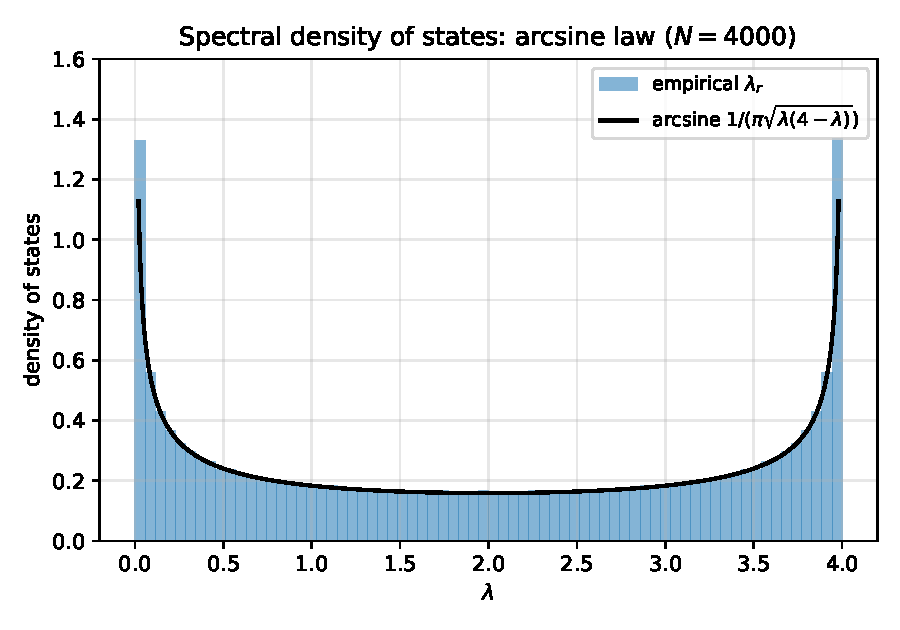
\includegraphics[width=.49\textwidth]{fig_dos.pdf}\hfill
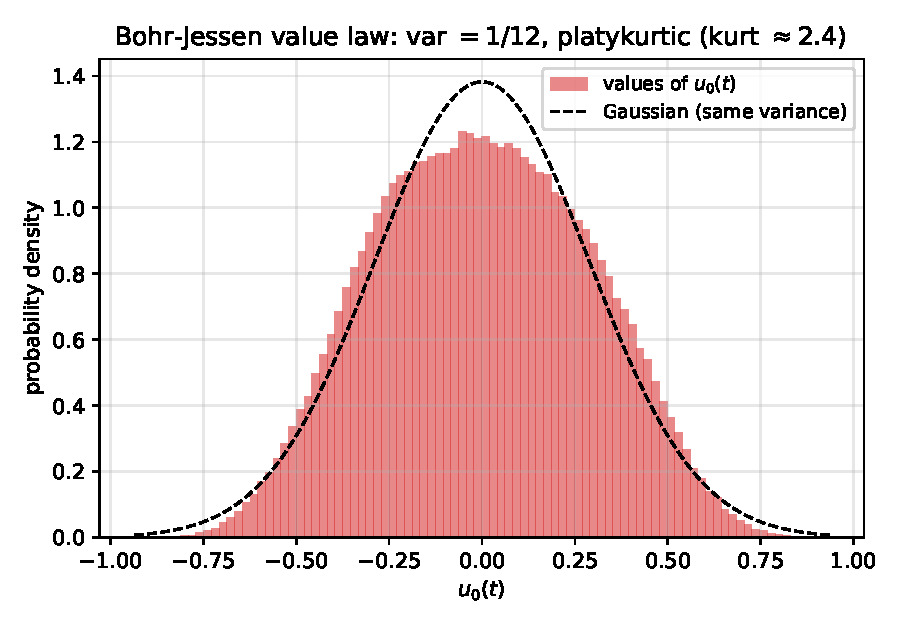
\includegraphics[width=.49\textwidth]{fig_value_dist.pdf}
\caption{Left: spectral density of states converges to the arcsine law \eqref{eq:arcsine}. Right: the
Bohr--Jessen value law of $u_0(t)$---symmetric, variance $(N^2-1)/(12N^2)\to1/12$, platykurtic (flatter
than the Gaussian of equal variance, dashed).}\label{fig:dos}
\end{figure}

\section{Higher-dimensional tori: the large wave is one-dimensional}\label{sec:dim}

On the $d$-dimensional torus $(\Z_N)^d$ the Laplacian is block-circulant-with-circulant-blocks (BCCB),
diagonalized by the $d$-dimensional DFT with eigenvalues
$\lambda_{\mathbf k}=\sum_{i=1}^d4\sin^2(\pi k_i/N)$ and $\omega_{\mathbf k}=\sqrt{\lambda_{\mathbf k}}$.
The triangle inequality gives, unconditionally,
$A_N^{(d)}\le U_N^{(d)}=N^{-d}\sum_{\mathbf k\ne\mathbf0}\omega_{\mathbf k}^{-1}$. Near the origin
$\omega_{\mathbf k}\sim(2\pi/N)|\mathbf k|$, so $N^d U_N^{(d)}$ mirrors the infrared lattice sum
$\sum 1/|\mathbf k|$, i.e.\ the integral $\int d^dk/|\mathbf k|$: logarithmically divergent for $d=1$
(giving $U_N\sim\frac1\pi\ln N$) but \emph{convergent} for $d\ge2$. Hence (Figure~\ref{fig:dimension})
\begin{equation}\label{eq:dim}
  U_N^{(d)}=\Theta(\ln N)\ \ (d=1),\qquad U_N^{(d)}=O(1)\ \ (d\ge2):
\end{equation}
the velocity Green's function---and with it the large-wave amplification---is \emph{uniformly bounded}
on the $2$- and $3$-torus. The large wave is intrinsically one-dimensional, a sharp dimensional
threshold set by the integrability of $1/\omega$ (\texttt{verify\_torus\_dimension.py}).

\medskip\noindent\textbf{Spectral dimension.} The threshold is not metric but \emph{spectral}. For
vertex-transitive (Fourier-flat) graph families the local ceiling reduces to the normalized spectral sum
$U_G=|V|^{-1}\sum_{\lambda_r>0}\lambda_r^{-1/2}$ ($\lambda_r$ the Laplacian spectrum,
$\omega_r=\sqrt{\lambda_r}$); for a general graph the ceiling at $(j,k)$ is
$\sum_{\lambda_r>0}|\phi_r(j)\phi_r(k)|\lambda_r^{-1/2}$ and also reflects eigenvector localization through
the local spectral measure, not the global density of states alone.
If the integrated density of states obeys $N(\lambda)\sim\lambda^{d_s/2}$ near $0$---defining the
\emph{spectral dimension} $d_s$---then $\rho(\lambda)\sim\lambda^{d_s/2-1}$ and
$U_G\sim\int_0\lambda^{-1/2}\rho(\lambda)\,d\lambda\sim\int_0\lambda^{(d_s-3)/2}\,d\lambda$, which
converges at the origin iff $d_s>1$. Hence the \emph{ceiling} $U_G$ grows logarithmically precisely at
the critical spectral dimension $d_s=1$, is bounded for $d_s>1$, and is power-law for $d_s<1$; the
$d$-torus is the case $d_s=d$. For $d_s>1$ this rigorously \emph{forbids} a large wave
($A_N\le U_G=O(1)$); at $d_s=1$ the ceiling permits one, but whether it is dynamically reached is the
same arithmetic reachability question as on the ring (Conjecture~\ref{conj:order}). The criterion is geometric rather than metric: any
\emph{quasi-one-dimensional} lattice---a ladder $C_N\times C_2$ or a tube $C_N\times C_w$ of bounded
width $w$---still has $d_s=1$ and retains a logarithmically divergent ceiling, now with reduced prefactor
$U_G\sim\tfrac1{\pi w}\ln N$ (only one of the $w$ transverse channels is gapless, Figure~\ref{fig:specdim}).
Bounded transverse width does not destroy the concentration; a genuine second extended dimension does
(\texttt{verify\_spectral\_dimension.py}).

\begin{figure}[ht]\centering
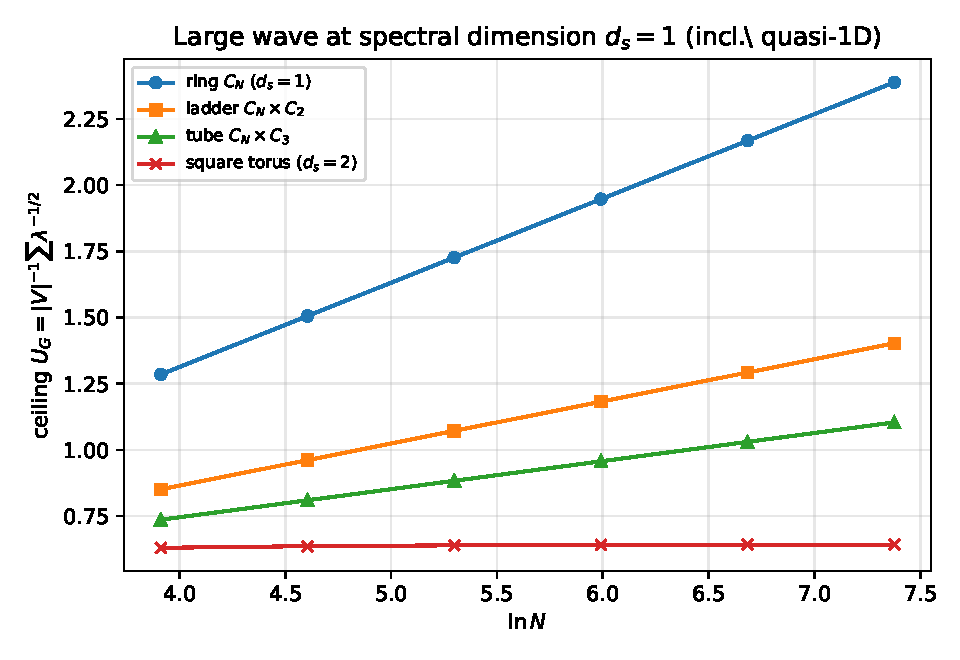
\includegraphics[width=.62\textwidth]{fig_spectral_dim.pdf}
\caption{Spectral-dimension threshold. The ceiling $U_G=|V|^{-1}\sum\lambda^{-1/2}$ grows like $\ln N$
for $d_s=1$---the ring and, with reduced slope $1/(\pi w)$, the quasi-1D ladder and tube---but saturates
for the $d_s=2$ square torus. The ceiling is a critical-dimension ($d_s=1$) phenomenon.}\label{fig:specdim}
\end{figure}

\begin{figure}[ht]\centering
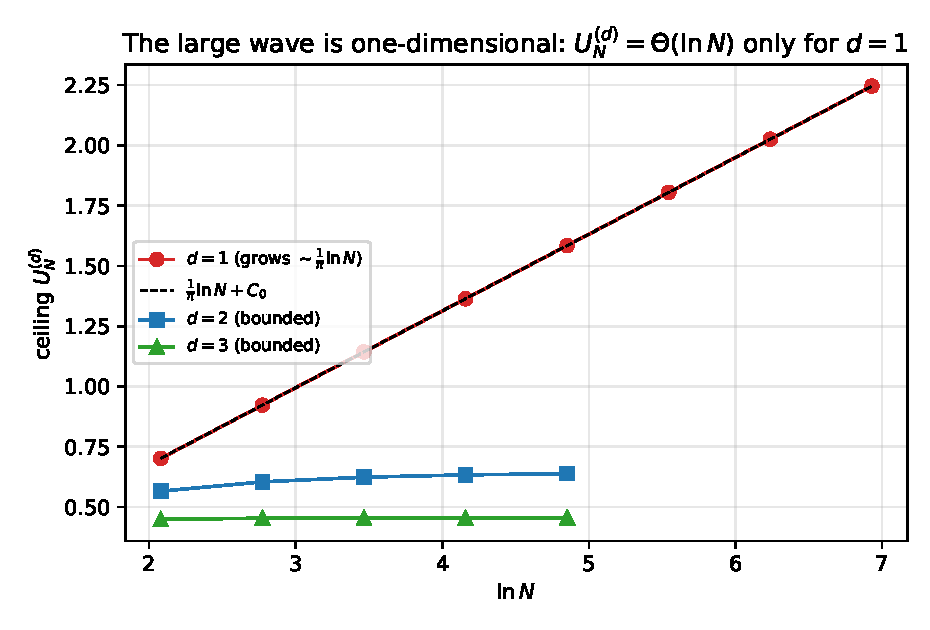
\includegraphics[width=.72\textwidth]{fig_dimension.pdf}
\caption{Ceilings $U_N^{(d)}$ versus $\ln N$. Only $d=1$ grows (slope $1/\pi$, on the dashed
$\frac1\pi\ln N+C_0$); the $2$- and $3$-torus ceilings saturate, so $A_N^{(d)}=O(1)$ for $d\ge2$.}
\label{fig:dimension}
\end{figure}


\part{Nonlinear extension}

% Part II --- Nonlinear extension.
% Included from large-wave-effect.tex; preamble macros (\LN, \Q, \eu, ...), \graphicspath and the
% bibliography all live in the root file. Add further nonlinear sections (breathers, FPUT, chaos) here.

\noindent\emph{The results of Part~II are primarily computational and exploratory. They outline natural
nonlinear continuations of the linear theory---and the energy-concentration thread that unifies
them---rather than claiming a complete nonlinear theory; each is reproduced by a verification script,
and the open analytical questions are flagged as such.}

\section{Rogue waves and the discrete NLS}\label{sec:rogue}

Restoring a cubic on-site interaction turns the linear Schr\"odinger ring of Section~\ref{sec:schr}
into the discrete nonlinear Schr\"odinger (DNLS) equation
\begin{equation}\label{eq:dnls}
  \mathrm i\,\dot z_j = -(\LN z)_j + \gamma\,|z_j|^2 z_j,\qquad \gamma>0\ \text{(focusing)},
\end{equation}
whose linear part is exactly $\LN$ and whose continuum limit (lattice spacing $\to0$, $\lambda_r\to k^2$)
is the \emph{focusing} nonlinear Schr\"odinger equation
\begin{equation}\label{eq:nls}
  \mathrm i\,\psi_t + \psi_{xx} + 2|\psi|^2\psi = 0,
\end{equation}
the canonical envelope model of deep-water and optical rogue waves~\cite{Zakharov,KharifPelinovsky,Onorato,Solli}.
(The literal limit is $\mathrm i\psi_t=\psi_{xx}+\gamma|\psi|^2\psi$, equal to \eqref{eq:nls} up to the
symmetry $\psi\mapsto\bar\psi$ and the rescaling $z\mapsto cz$ that sets $\gamma=2$.) Thus the very operator $\LN$ that
governs the linear large wave sits at the heart of the rogue-wave problem, and the two amplification
mechanisms can be compared on the same lattice (\texttt{verify\_rogue\_dnls.py}).

\begin{proposition}[Hamiltonian structure and conservation]\label{prop:dnls-cons}
The DNLS \eqref{eq:dnls} is Hamiltonian, $\mathrm i\dot z_j=\partial H/\partial\bar z_j$ with
\[
  H(z)=-\sum_j|z_{j+1}-z_j|^2+\frac\gamma2\sum_j|z_j|^4,
\]
and conserves both $H$ and the power $P(z)=\sum_j|z_j|^2$; consequently the flow is global and
norm-preserving on $\mathbb C^N$.
\end{proposition}

\begin{proof}
$\tfrac{d}{dt}P=2\,\mathrm{Re}\sum_j\dot z_j\bar z_j
 =2\,\mathrm{Re}\bigl[-\mathrm i\bigl(\langle\LN z,z\rangle-\gamma\textstyle\sum_j|z_j|^4\bigr)\bigr]=0$,
since $\langle\LN z,z\rangle$ and $\sum_j|z_j|^4$ are real (so $-\mathrm i(\cdot)$ is purely imaginary); and
$\partial H/\partial\bar z_j=(z_{j+1}+z_{j-1}-2z_j)+\gamma|z_j|^2z_j=-(\LN z)_j+\gamma|z_j|^2z_j$, so
$\mathrm i\dot z=\partial H/\partial\bar z$ and $H$ is conserved along the flow. With $P$ bounded, no
finite-time blow-up occurs. Both invariants are reproduced numerically: the norm-preserving split-step
integrator holds $P$ to $10^{-12}$ and $H$ to $O(\Delta t^2)$ (\texttt{verify\_dnls\_selftrapping.py}).
\end{proof}

\emph{Peregrine soliton.} Equation~\eqref{eq:nls} possesses the rational solution~\cite{Peregrine}
\begin{equation}\label{eq:peregrine}
  \psi_P(x,t) = \left[\,1 - \frac{4(1+4\mathrm i t)}{1+4x^2+16t^2}\,\right]\eu^{2\mathrm i t},
\end{equation}
localized in both space and time, with unit background $|\psi|\to1$ and peak $|\psi_P(0,0)|=3$: the
threefold amplification ``appearing from nowhere and disappearing without a trace'' that defines a
rogue wave (Figure~\ref{fig:peregrine}). We verified that \eqref{eq:peregrine} solves \eqref{eq:nls}
to a PDE residual vanishing under grid refinement. The Peregrine breather is the limit of the
space-periodic Akhmediev and time-periodic Kuznetsov--Ma breather families produced by the Darboux
transformation~\cite{Akhmediev}. These exact breathers exist because the focusing NLS \eqref{eq:nls}
is \emph{completely integrable}---the compatibility condition of the Zakharov--Shabat linear system,
solved by the inverse scattering transform~\cite{ZakharovShabat}, on which the Darboux dressing rests.

\emph{Modulational instability.} The seed of these structures is the Benjamin--Feir
instability~\cite{BenjaminFeir,ZakharovOstrovsky}, the mechanism by which Zakharov's deep-water
envelope equation~\cite{Zakharov} destabilizes a uniform train. The uniform train
$z_j=A\,\eu^{-\mathrm i\gamma A^2 t}$ solves \eqref{eq:dnls} ($\LN\mathbf1=0$); writing
$z_j=[A+p_j(t)]\eu^{-\mathrm i\gamma A^2 t}$ and keeping terms linear in $p$, the cubic contributes
$\gamma A^2(2p_j+\bar p_j)$, leaving
\[
  \mathrm i\dot p_j=-(\LN p)_j+\gamma A^2(p_j+\bar p_j).
\]
The Fourier ansatz $p_j=u\,\eu^{\mathrm i\kappa j+\sigma t}+\bar v\,\eu^{-\mathrm i\kappa j+\sigma t}$
(eigenvalue $\lambda_\kappa$ of $\LN$ on $\eu^{\mathrm i\kappa j}$) reduces this to the $2\times2$ system
$\mathrm i\sigma u=(\gamma A^2-\lambda_\kappa)u+\gamma A^2v$, $-\mathrm i\sigma v=\gamma A^2u+(\gamma A^2-\lambda_\kappa)v$,
whose solvability condition $\sigma^2+(\gamma A^2-\lambda_\kappa)^2=(\gamma A^2)^2$ gives the growth rate
\begin{equation}\label{eq:mi}
  \sigma(\kappa)=\sqrt{\lambda_\kappa\,(2\gamma A^2-\lambda_\kappa)},\qquad \lambda_\kappa=4\sin^2\tfrac\kappa2,
\end{equation}
so the band $\lambda_\kappa<2\gamma A^2$ is unstable (continuum form $\sigma=|k|\sqrt{2\gamma A^2-k^2}$, the
classical $|k|\sqrt{4A^2-k^2}$ at $\gamma=2$). This linear-stability computation is exact:

\begin{proposition}[modulational-instability band]\label{prop:mi}
The uniform state $z_j=A\,\eu^{-\mathrm i\gamma A^2t}$ of \eqref{eq:dnls} is linearly unstable to the
Fourier mode $\kappa$ if and only if $\lambda_\kappa<2\gamma A^2$, with growth rate
$\sigma(\kappa)=\sqrt{\lambda_\kappa(2\gamma A^2-\lambda_\kappa)}$; the rate is maximal,
$\sigma_{\max}=\gamma A^2$, at $\lambda_\kappa=\gamma A^2$.
\end{proposition} A direct split-step simulation of \eqref{eq:dnls} reproduces
\eqref{eq:mi} to better than $1\%$ across the band interior (Figure~\ref{fig:mi}); the fastest mode
does not grow without bound but develops into a recurrent breather-like modulation reminiscent of the
Akhmediev scenario of the continuum integrable NLS---a periodic avatar of the rogue spike.

\emph{From thin tails to heavy tails.} The statistical signature is the sharpest contrast with the
linear theory. Seeded by a noisy plane wave, \eqref{eq:dnls} on the ring spawns localized bursts exceeding an operational envelope threshold of twice
the root-mean-square amplitude (analogous to common rogue-wave criteria)---and the amplitude
distribution develops a heavy, \emph{leptokurtic} tail (kurtosis $>3$) lying well above the Rayleigh
law of a linear Gaussian sea (Figure~\ref{fig:rogue}). This inverts the linear picture, whose
Bohr--Jessen value law is \emph{platykurtic} (Section~\ref{sec:stats}): linear amplification is a rare
phase alignment of bounded, thin-tailed oscillations, whereas nonlinear focusing manufactures genuine
heavy-tailed extremes. The two regimes share the lattice operator $\LN$ but reach large amplitudes by
opposite routes---interference versus self-focusing.

A rigorous nonlinear theory on the ring---existence and stability of discrete breathers, the precise
role of the $\LN$ spectrum in the instability band, and integrable discretizations of
\eqref{eq:nls}---is left to future work; equation~\eqref{eq:dnls} is recorded here as the natural
nonlinear continuation of the linear large wave.

\begin{figure}[ht]\centering
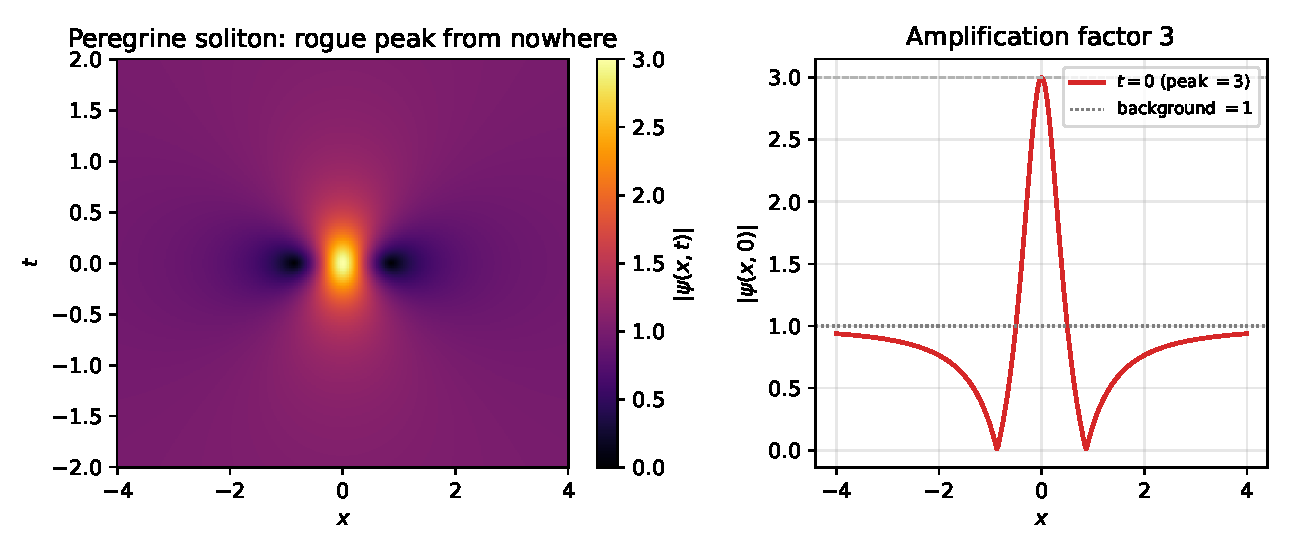
\includegraphics[width=.86\textwidth]{fig_peregrine.pdf}
\caption{Peregrine soliton~\eqref{eq:peregrine} of the focusing NLS~\eqref{eq:nls}: a rogue peak
localized in space and time (left), with the threefold amplification over the unit background at
$t=0$ (right).}\label{fig:peregrine}
\end{figure}

\begin{figure}[ht]\centering
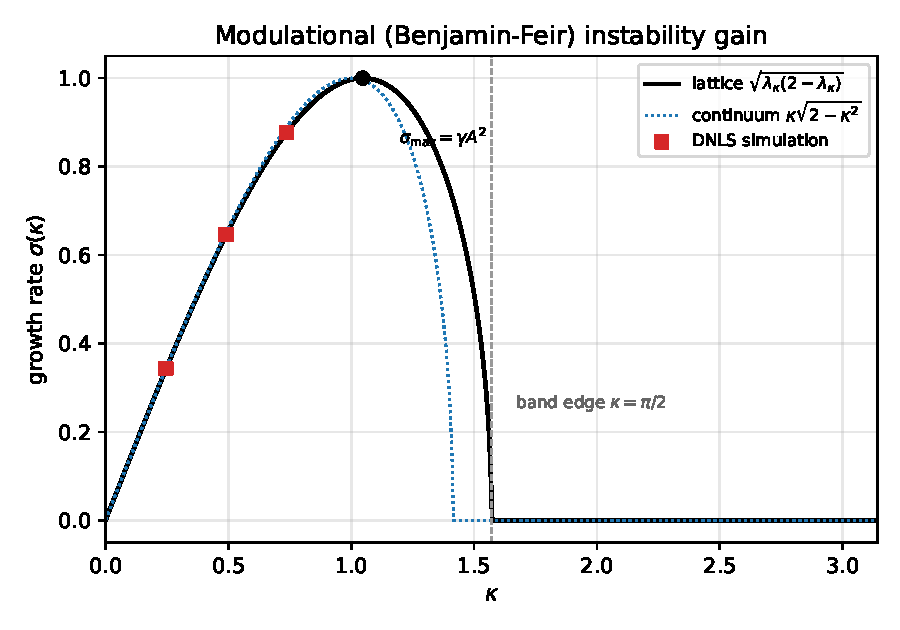
\includegraphics[width=.66\textwidth]{fig_mi.pdf}
\caption{Modulational (Benjamin--Feir) instability gain~\eqref{eq:mi} of the plane wave under the
DNLS~\eqref{eq:dnls}: lattice rate (solid), continuum approximation (dotted) and simulated growth
rates (squares), with unstable band edge $\kappa=\pi/2$ and maximal rate
$\sigma_{\max}=\gamma A^2$.}\label{fig:mi}
\end{figure}

\begin{figure}[ht]\centering
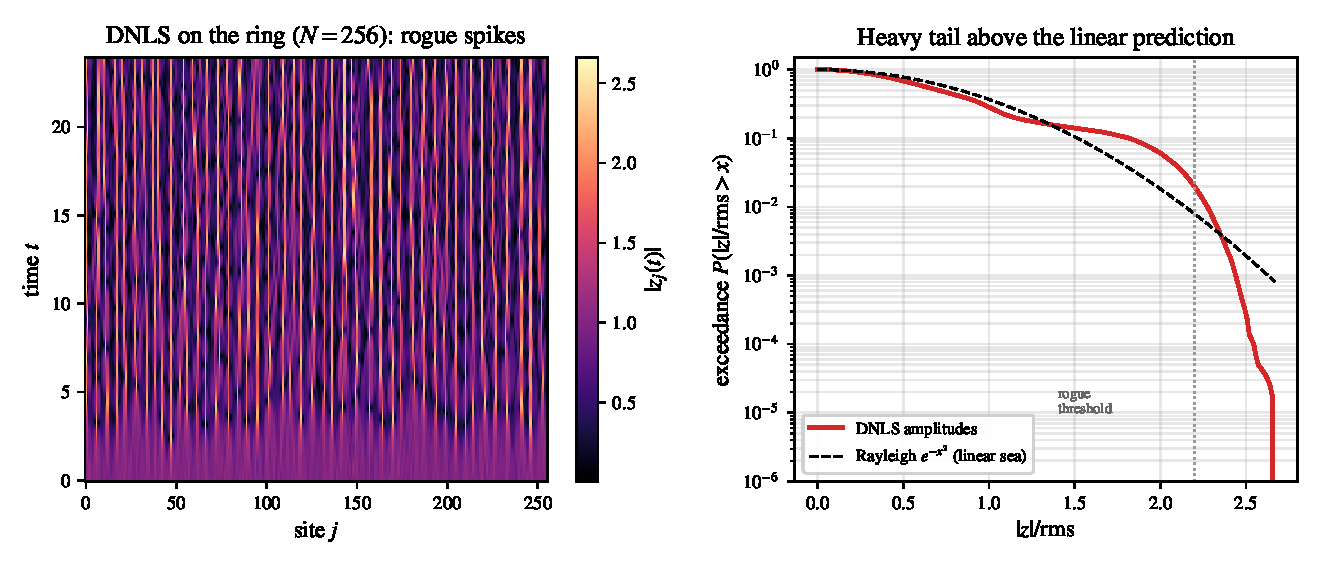
\includegraphics[width=.92\textwidth]{fig_rogue_dnls.pdf}
\caption{DNLS~\eqref{eq:dnls} on the ring seeded by a noisy plane wave. Left: space-time amplitude
$|z_j(t)|$ with localized rogue spikes. Right: the amplitude exceedance distribution develops a heavy
tail above the Rayleigh law (dashed) of a linear Gaussian sea, crossing the rogue threshold---the
opposite of the platykurtic linear value law.}\label{fig:rogue}
\end{figure}

\section{Discrete breathers and self-trapping}\label{sec:breather}

Nonlinearity does not only sharpen extremes; it can \emph{localize}. Seed the DNLS \eqref{eq:dnls} with a
single excited site, $z_j(0)=A\,\delta_{j0}$ (norm $\Lambda=\sum_j|z_j|^2=A^2$), and track the
\emph{participation ratio}
\begin{equation}\label{eq:pr}
  P=\frac{\bigl(\sum_j|z_j|^2\bigr)^2}{\sum_j|z_j|^4}\in[1,N],
\end{equation}
which is $1$ for a single occupied site and $\sim N$ when the excitation spreads over the ring. A
norm-conserving split-step integrator (norm exact to $10^{-12}$, $H$ to $O(\Delta t^2)$) shows a sharp
\emph{self-trapping transition} at the on-site nonlinear frequency $\gamma|z_0|^2\approx4$---exactly the
top of the spectrum of $\LN$, the band $[0,4]$. Below it the excitation disperses ($P\to N$); above it the
site detunes out of the linear band and forms a long-lived, exponentially localized \emph{breather-like
state} $z_j(t)\approx\phi_j\eu^{-\mathrm i\Omega t}$ consistent with the stationary DNLS branch, whose real profile solves
$\Omega\phi_j=-(\LN\phi)_j+\gamma\phi_j^3$ with frequency $\Omega\approx\gamma|z_0|^2$ pushed above the
whole phonon band $[0,4]$, so no extended mode can resonate (Figure~\ref{fig:selftrapping}; the trapped
profile is steady, the temporal standard deviation of $|z_j|$ staying below $0.02$). This is the dynamical
\emph{opposite} of the linear large wave, a fully delocalized interference of all $N$ modes ($P\sim N$):
the same operator $\LN$ supports both a spread-out resonance (linear) and a pinned soliton (nonlinear),
selected by the size of the cubic term (\texttt{verify\_dnls\_selftrapping.py}).

\emph{Two thresholds.} An anti-continuum estimate places the \emph{stationary} single-site breather at
$\gamma|\phi_0|^2\gtrsim2$: from $\Omega\phi_j=-(\LN\phi)_j+\gamma\phi_j^3$ with $\phi\approx\sqrt P\,\delta_{j0}$
one gets $\Omega\approx\gamma P-2$, which clears the band \emph{top} ($\Omega>0$) at $\gamma P\gtrsim2$. The
larger \emph{dynamical} threshold $\gamma|z_0|^2\approx4$ measured from a single-site \emph{launch} is the
bandwidth: the spreading excitation must outrun the entire band $[0,4]$, not merely its edge. Existence and
stability of these breathers (MacKay--Aubry theory~\cite{MacKayAubry}) and the precise dynamical threshold
are the rigorous sequel left open here.

\begin{figure}[ht]\centering
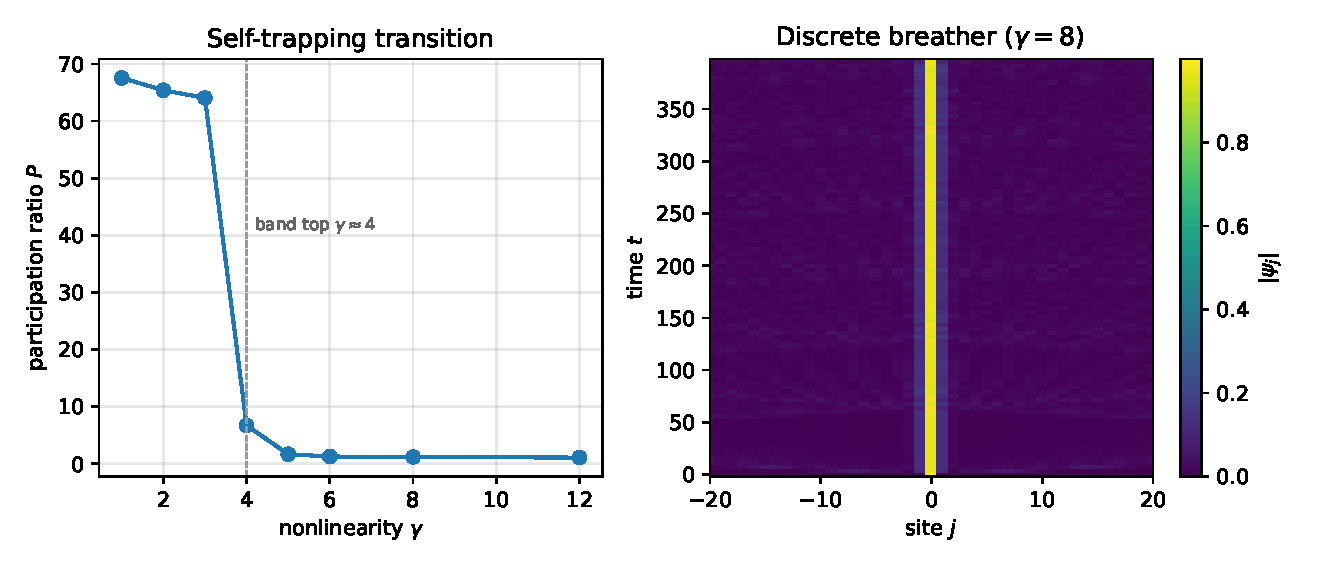
\includegraphics[width=.92\textwidth]{fig_selftrapping.pdf}
\caption{DNLS self-trapping ($N=128$, single-site seed). Left: the participation ratio $P$ collapses from
$\sim N$ (dispersed) to $\sim1$ (trapped) as the nonlinearity crosses the band top $\gamma\approx4$.
Right: above threshold the excitation is a persistent localized breather-like state---a localized column in
space-time.}\label{fig:selftrapping}
\end{figure}

\section{FPUT recurrence and the route to chaos}\label{sec:chaos}

The cubic coupling also makes the lattice a testbed for Hamiltonian chaos. The
Fermi--Pasta--Ulam--Tsingou (FPUT) $\beta$-ring
\begin{equation}\label{eq:fput}
  \ddot u_j=(u_{j+1}-2u_j+u_{j-1})+\beta\bigl[(u_{j+1}-u_j)^3-(u_j-u_{j-1})^3\bigr]
\end{equation}
has linear part $\ddot u=-\LN u$ and Hamiltonian
$H=\sum_j\bigl[\tfrac12\dot u_j^2+\tfrac12(u_{j+1}-u_j)^2+\tfrac{\beta}{4}(u_{j+1}-u_j)^4\bigr]$. Seeding
all energy in mode~$1$ and integrating symplectically (velocity Verlet; $H$ conserved to $6\times10^{-4}$
with no secular drift), at low energy the energy does \emph{not} thermalize: it sloshes to a few
neighbouring modes and \emph{returns} to mode~$1$---the FPUT recurrence (Figure~\ref{fig:fput}), the
near-integrable face of the nonlinear lattice: its long-wave limit is a Korteweg--de Vries-type
equation, a completely integrable Hamiltonian system~\cite{ZakharovFaddeev} whose invariant tori the
weakly nonlinear lattice shadows, so energy returns rather than equipartitioning. Only a handful of low
modes are ever active, the dynamics
is quasi-periodic, and the maximal Lyapunov exponent is $\lambda_{\max}\approx0$---just as for the
integrable linear large wave.

Raising the energy breaks integrability. Measured by the Benettin method (a tangent vector co-evolved
with the variational equations and periodically renormalized,
$\lambda_{\max}=T^{-1}\sum\log\lVert\delta\rVert/d_0$), the maximal Lyapunov exponent turns on with
energy (Figure~\ref{fig:lyapunov}): $\lambda_{\max}\approx0.001$ in the regular regime, rising through a
weak-chaos knee to $\lambda_{\max}\approx0.05$ in the strongly chaotic regime, where the energy
thermalizes across all modes. The same lattice---linear core $\LN$---thus interpolates between integrable
tori and deterministic chaos as the amplitude grows (\texttt{verify\_fput\_recurrence.py},
\texttt{verify\_lyapunov.py}). The transition is visible directly in phase space: in the three
odd-mode energy coordinates $(E_1,E_3,E_5)$ (a mode-$1$ seed excites only odd modes by parity) the orbit
lies on a thin quasi-periodic torus at low energy and fills a chaotic cloud at high energy
(Figure~\ref{fig:phase3d}).

\begin{figure}[ht]\centering
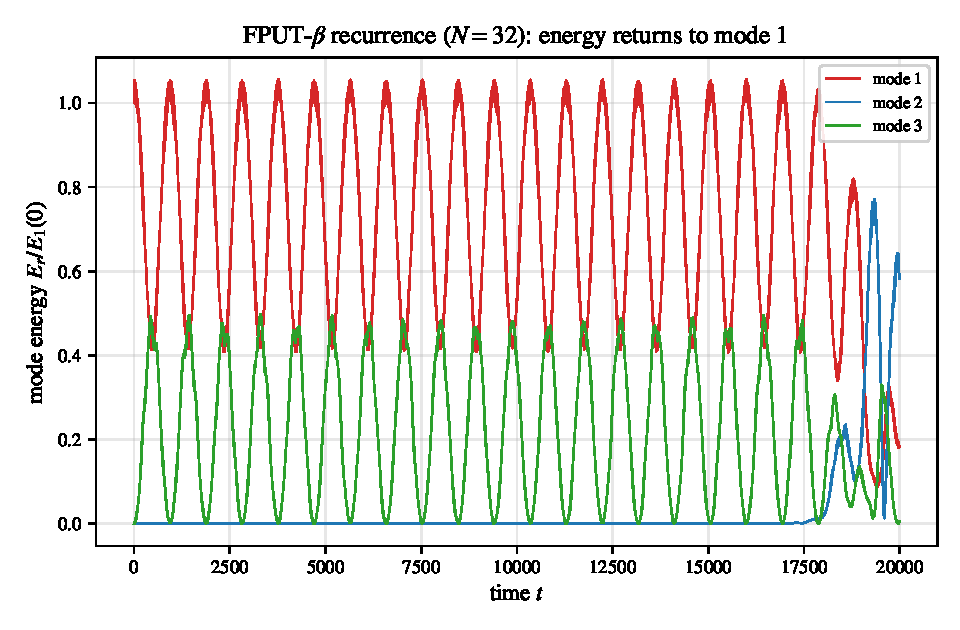
\includegraphics[width=.72\textwidth]{fig_fput.pdf}
\caption{FPUT-$\beta$ recurrence ($N=32$, mode-1 seed). The harmonic energy of mode~$1$ drops almost to
zero and recurs to its initial value, sloshing quasi-periodically with the low modes instead of
thermalizing.}\label{fig:fput}
\end{figure}

\begin{figure}[ht]\centering
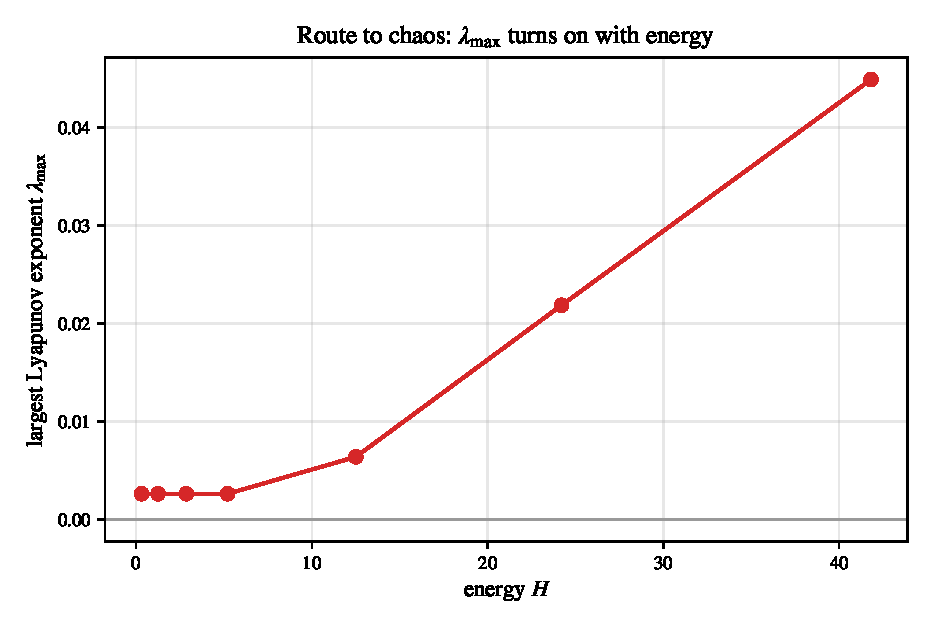
\includegraphics[width=.66\textwidth]{fig_lyapunov.pdf}
\caption{Route to chaos. The maximal Lyapunov exponent of the FPUT-$\beta$ ring is $\approx0$ at low
energy (regular, the recurrence regime) and turns on past an energy threshold, reaching
$\lambda_{\max}\approx0.05$ in the chaotic regime.}\label{fig:lyapunov}
\end{figure}

\begin{figure}[ht]\centering
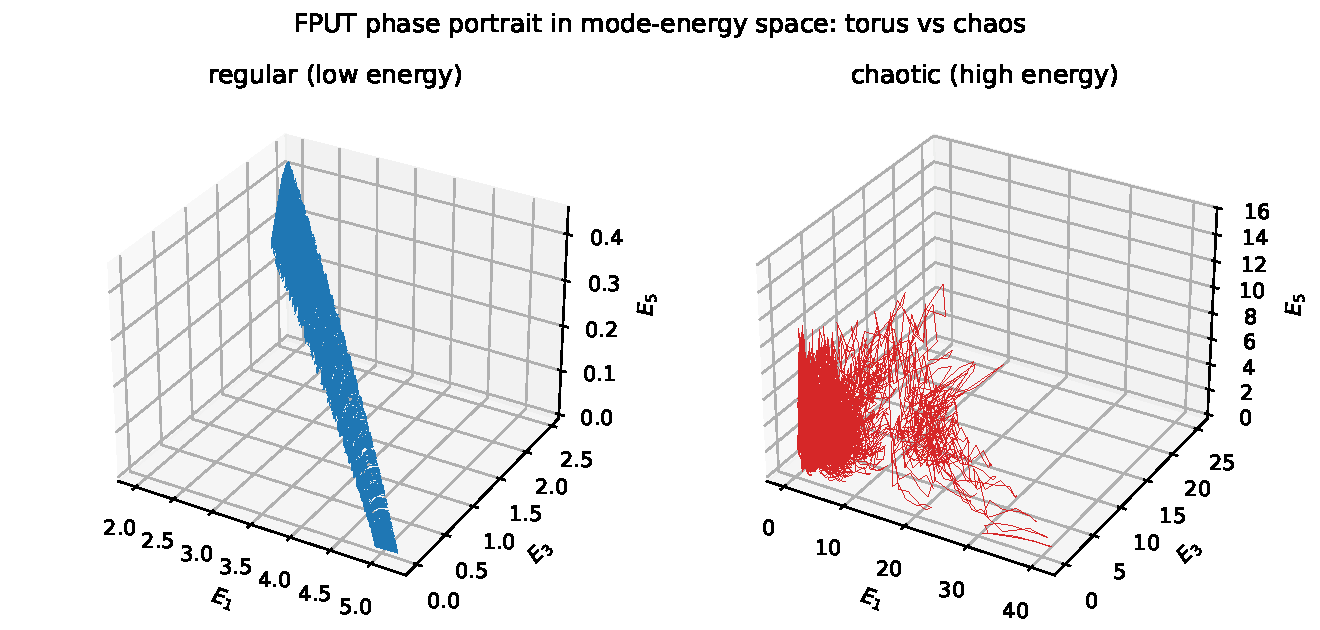
\includegraphics[width=.92\textwidth]{fig_phase3d.pdf}
\caption{FPUT phase portrait in the odd-mode energy space $(E_1,E_3,E_5)$. Left: at low energy the orbit
lies on a thin quasi-periodic torus (regular). Right: at high energy it fills a three-dimensional
chaotic cloud---the same regular-to-chaotic transition measured by $\lambda_{\max}$.}\label{fig:phase3d}
\end{figure}

\section{Diagnostics and the fate of the large wave}\label{sec:fate}

The linear large wave and its nonlinear continuations are cleanly separated by a small set of dynamical
diagnostics---localization (participation ratio $P$), value statistics (kurtosis $\kappa$) and chaos
(Lyapunov exponent $\lambda_{\max}$)---all built on the \emph{same} lattice operator $\LN$
(Table~\ref{tab:diagnostics}). The linear large wave is a delocalized, thin-tailed, integrable resonance
($P\sim N$, $\kappa<3$, $\lambda_{\max}=0$); nonlinearity opens three distinct routes to a large local
amplitude---\emph{self-focusing} into rogue extremes (heavy tails, $\kappa>3$), \emph{self-trapping} into
a pinned breather ($P\sim1$), and \emph{chaotic} thermalization ($\lambda_{\max}>0$). Which one is
realized is set by the sign and strength of the nonlinearity and by the energy; the linear theory of
Part~I is the $\beta,\gamma\to0$ corner of this picture, and supplies the spectral data ($\LN$, the band
$[0,4]$, the modal frequencies) that organize every regime. A rigorous nonlinear theory on the
ring---existence and stability of the discrete breathers, the precise role of the $\LN$ spectrum in the
modulational band, and the energy threshold for chaos---is the natural sequel.

\begin{table}[ht]\centering
\caption{The large wave and its nonlinear continuations, separated by dynamical diagnostics on the common
operator $\LN$. ($P$: participation ratio; $\kappa$: kurtosis; $\lambda_{\max}$: largest Lyapunov
exponent; ``---'' marks a diagnostic not characteristic of that regime.)}\label{tab:diagnostics}
\begin{tabular}{lllll}
\hline
Regime & Model & Localization $P$ & Statistics $\kappa$ & $\lambda_{\max}$\\
\hline
Linear large wave & $\ddot u=-\LN u$ & delocalized $\sim N$ & platykurtic $<3$ & $0$\\
Rogue / self-focusing & DNLS, noisy plane wave & localized bursts & leptokurtic $>3$ & ---\\
Discrete breather & DNLS, $\gamma|z_0|^2>4$ & pinned $\sim1$ & --- & $0$\\
FPUT recurrence & FPUT-$\beta$, low $E$ & few active modes & --- & $\approx0$\\
Chaos & FPUT-$\beta$, high $E$ & thermalized $\sim N$ & --- & $>0$\\
\hline
\end{tabular}
\end{table}

\section{Higher dimensions: nonlinear localization beyond the one-dimensional large wave}\label{sec:highd}

Part~I established that the \emph{linear} large wave is one-dimensional: on the $d$-torus the ceiling
$U_N^{(d)}$ is bounded for $d\ge2$ (Section~\ref{sec:dim}), so a localized linear disturbance cannot
amplify in two or three dimensions. Nonlinearity removes the obstruction. On the $2$-torus $(\Z_N)^2$
the DNLS with the block-circulant Laplacian $\LN^{(2)}$ (eigenvalues
$\lambda_{\mathbf r}=4\sin^2\frac{\pi r_1}{N}+4\sin^2\frac{\pi r_2}{N}$, band $[0,8]$, with the
dispersion surface of Figure~\ref{fig:dispersion3d}) self-traps a single-site excitation into a
long-lived, exponentially localized \emph{two-dimensional breather-like state} once the on-site nonlinear
frequency crosses the $2$D band top, $\gamma|z|^2\approx8$: the norm is conserved to $10^{-12}$ and the
participation ratio collapses from $\sim N^2$ to $O(1)$ across the threshold
(Figure~\ref{fig:breather2d}, \texttt{verify\_dnls\_2d.py}). A large, localized amplitude therefore
survives in $2$D (and, identically, $3$D) by a mechanism---self-focusing self-trapping---absent from the
linear theory: the dimensional threshold of Part~I is a property of the \emph{linear} resonance, not of
the lattice.

This multidimensional, strongly nonlinear regime points toward Zakharov's wider program: a possible
multidimensional long-wave asymptotic direction is the Zakharov--Kuznetsov regime~\cite{ZakharovKuznetsov}
(we do not carry out the multiscale derivation from \eqref{eq:fput} here), and the statistics of the
thermalizing lattice suggest a connection to the weak-turbulence (Kolmogorov--Zakharov) theory of wave
spectra~\cite{ZakharovLvovFalkovich}. The rigorous wave-kinetic results of~\cite{DengHani} concern a
different weakly nonlinear, large-box scaling (dimension $d\ge3$) and do not directly justify the finite
one-dimensional lattice here. These
connect the discrete large-wave problem to the broad theory of nonlinear wave dynamics
(Section~\ref{sec:fate}).

\begin{figure}[ht]\centering
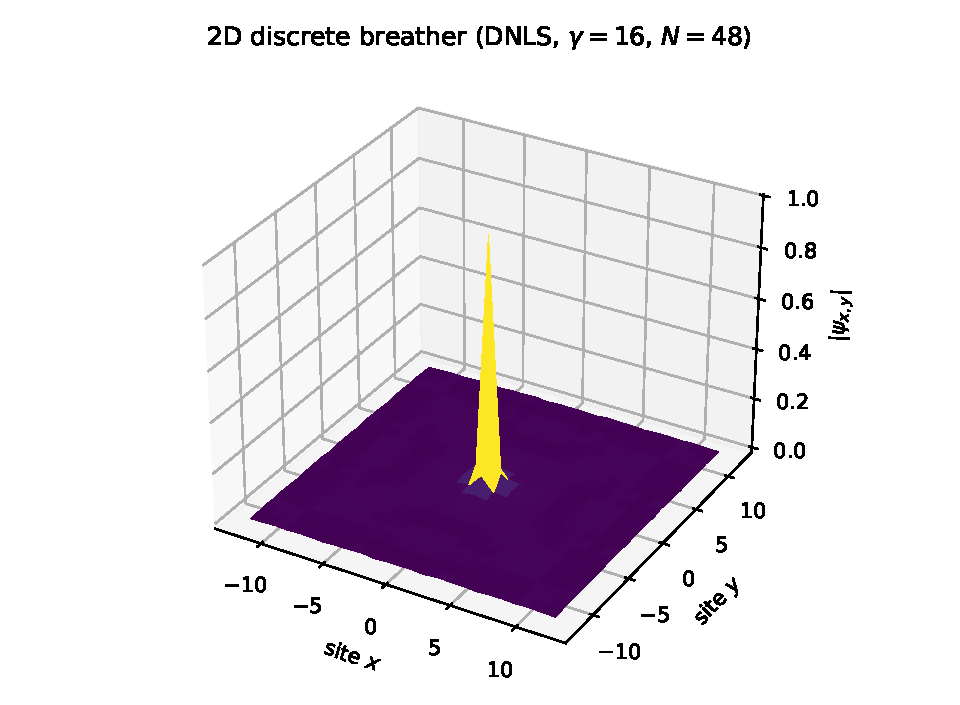
\includegraphics[width=.6\textwidth]{fig_breather2d.pdf}
\caption{Two-dimensional discrete breather: a single-site seed under the $2$D DNLS self-traps into a
persistent localized hump above the $2$D band top ($\gamma\approx8$). Nonlinearity restores a large
localized amplitude in $2$D, where the linear large wave is bounded.}\label{fig:breather2d}
\end{figure}

\begin{figure}[ht]\centering
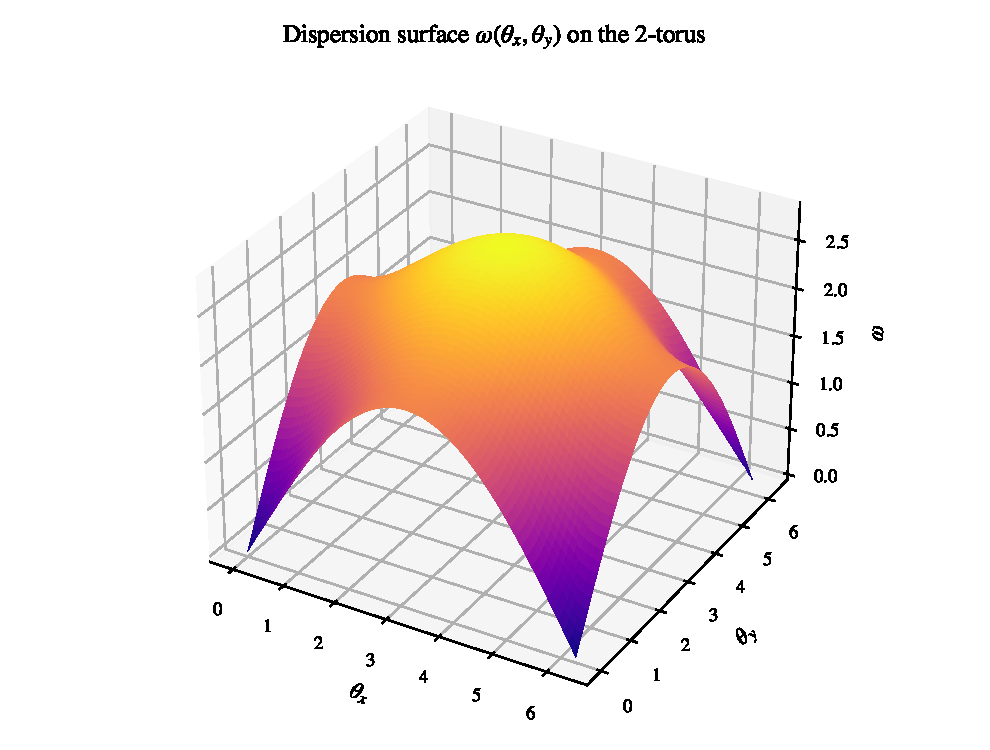
\includegraphics[width=.58\textwidth]{fig_dispersion3d.pdf}
\caption{Dispersion surface
$\omega(\theta_x,\theta_y)=2\sqrt{\sin^2(\theta_x/2)+\sin^2(\theta_y/2)}$ of the block-circulant
Laplacian on the $2$-torus: zero at the corners, band top $2\sqrt2$ at the centre.}\label{fig:dispersion3d}
\end{figure}

\section{Caustics and the concentration of energy}\label{sec:caustic}

The thread running through this paper is the \emph{concentration of energy} into a large local
amplitude. Part~I concentrates it by modal interference (the linear large wave); Part~II so far by
nonlinear self-focusing (rogue waves, breathers). A third, purely \emph{linear} route is refractive: in
a slowly varying medium a wave follows rays $\dot{\mathbf x}=\nabla_{\mathbf k}\omega$,
$\dot{\mathbf k}=-\nabla_{\mathbf x}\omega$, and where neighbouring rays cross, the ray density---and with
it the amplitude---diverges on a \emph{caustic}. Caustics are classified by catastrophe
theory~\cite{BerryUpstill}: the generic fold (Airy diffraction) and cusp (the bright curve at the bottom
of a teacup); diffraction regularizes the divergence to a finite but large peak with a universal scaling.

\emph{Rays and their envelopes.} Geometric optics is the skeleton. For waves crossing a current the
Doppler term refracts the rays, and a bundle of initially parallel rays entering a current jet
converges and \emph{folds}: its Jacobian $\partial x/\partial x_0$ passes through zero at a finite
focal distance, where the ray density $1/|\partial x/\partial x_0|$---and with it the linear
amplitude---diverges, regularized by diffraction (Figure~\ref{fig:raycaustic},
\texttt{verify\_ray\_caustic.py}).

\begin{figure}[ht]\centering
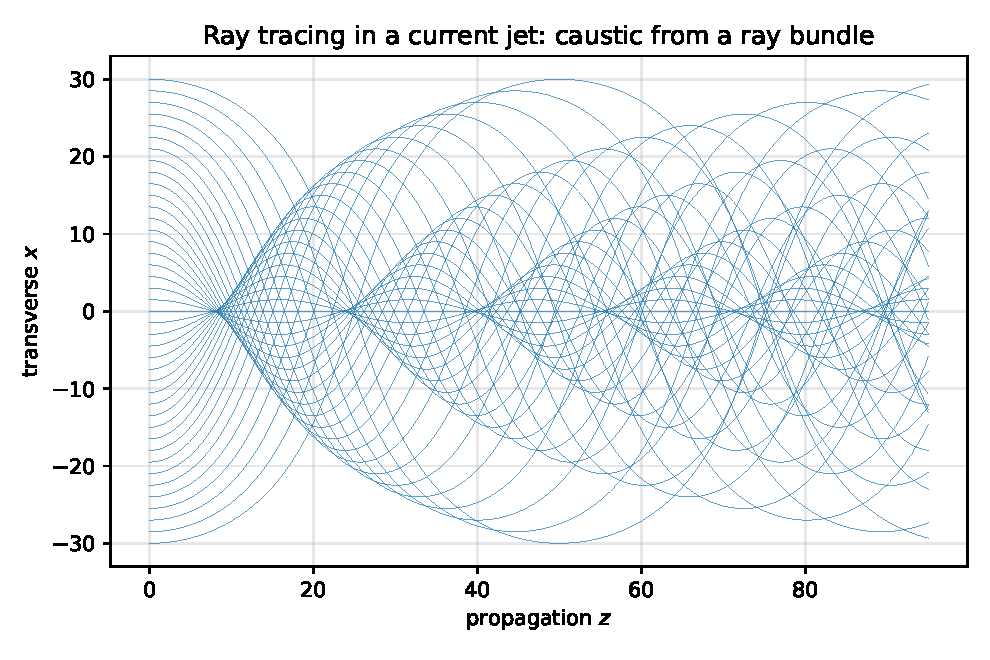
\includegraphics[width=.66\textwidth]{fig_raycaustic.pdf}
\caption{Ray tracing in a current jet. A bundle of parallel rays is refracted toward the jet, crosses
on a caustic (the fold near $z\approx8$, then re-focusing), where the ray density and the linear
amplitude concentrate.}\label{fig:raycaustic}
\end{figure}

\emph{The discrete front is a caustic.} The lattice already contains one. For the discrete Schr\"odinger
equation (Section~\ref{sec:schr}) the group velocity $v_g(k)=2\sin k$ is extremal at $k=\tfrac\pi2$---a
degenerate stationary-phase point, a fold---so the propagator front is exactly the Airy function,
\begin{equation}\label{eq:airy}
  J_n(2t)\sim t^{-1/3}\,\mathrm{Ai}\!\Bigl(2^{1/3}\,\tfrac{n-2t}{(2t)^{1/3}}\Bigr),
\end{equation}
with the universal fold scaling $\max_n|J_n(2t)|\sim0.536\,t^{-1/3}$ (Figure~\ref{fig:caustic},
\texttt{verify\_caustic\_airy.py}). The discrete large-wave front \emph{is} a fold caustic, the
$t^{-1/3}$ being the Airy exponent.

\emph{The cusp and the teacup.} The next generic caustic is the \emph{cusp}---the bright curve at the
bottom of a sunlit teacup, whose ray version (parallel rays reflected inside a circle) is a
\emph{nephroid} and whose universal diffraction is the Pearcey integral
$\mathrm{Pe}(X,Y)=\int_{-\infty}^{\infty}\exp\!\bigl[\mathrm i(s^4+Xs^2+Ys)\bigr]\,\mathrm ds$ over the
cusp catastrophe, with geometric caustic $8X^3+27Y^2=0$. Its cusp-point value is
$|\mathrm{Pe}(0,0)|=\tfrac12\Gamma(\tfrac14)=1.8128$, and the intensity concentrates inside the cusp and
falls off in the geometric shadow (Figure~\ref{fig:cusp}, \texttt{verify\_cusp\_pearcey.py}).

\begin{figure}[ht]\centering
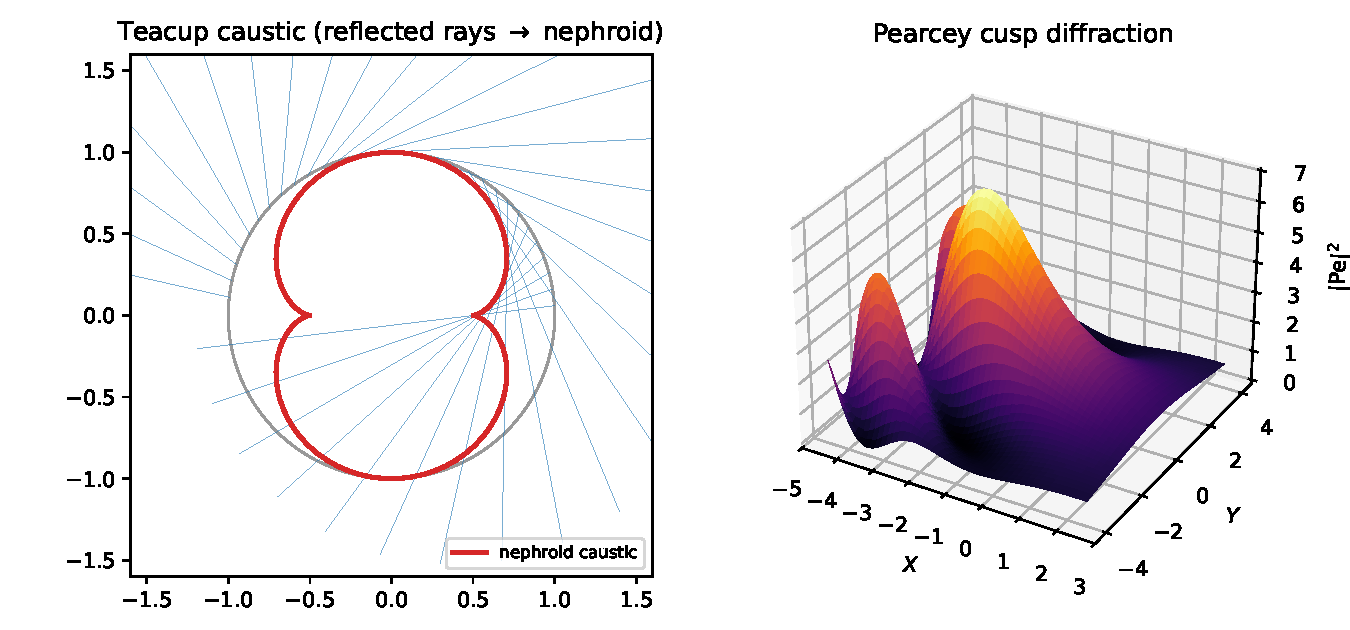
\includegraphics[width=.92\textwidth]{fig_cusp.pdf}
\caption{The cusp caustic. Left: the everyday teacup caustic---parallel rays reflected inside a circle
have a nephroid envelope. Right: the universal Pearcey diffraction $|\mathrm{Pe}(X,Y)|^2$ of the cusp,
bright inside the cusp and dark in the shadow.}\label{fig:cusp}
\end{figure}

\emph{Ocean rogue hot spots.} The same refraction sets the geography of ocean rogue waves. Swell from
Southern-Ocean storms running into the opposing Agulhas current off south-east Africa is refracted and
focused into caustics---the classic rogue ``hot spot''~\cite{Lavrenov,WhiteFornberg,Slunyaev}. A spatially random
current produces a cascade of caustics, \emph{branched flow}: a uniform incident wave develops bright
filaments and focal hot spots whose intensity is heavy-tailed, the linear precursor of rogue
statistics~\cite{YingHeller}. The paraxial model
$\mathrm i\,\partial_z\psi=-\tfrac12\partial_{xx}\psi+V(x)\psi$ with a weak random current $V$ reproduces
it exactly (Figure~\ref{fig:branched}): from a flat wave the scintillation index
$\max_x|\psi|^2/\langle|\psi|^2\rangle$ rises from $1$ to ${\sim}13$ at a focal distance, and the
focal-plane intensity is heavy-tailed---its tail an order of magnitude above the exponential law of a
structureless field (\texttt{verify\_branched\_flow.py}). Tidal (lunar) currents modulate the refracting
flow, a secondary effect.

\emph{The lens seeds self-focusing.} The two routes cooperate. A linear caustic concentrates energy
until the local steepness crosses the modulational threshold, whereupon nonlinear self-focusing takes
over---rogue waves are ``the nonlinear stage of the modulational instability''~\cite{ZakharovShamin}.
Seeding the focusing NLS with a converging (lens) beam (Figure~\ref{fig:caustic_mi}), the linear caustic
amplifies a weak flat input ${\sim}7\times$, and the nonlinearity then sharpens the focal peak by a
further ${\sim}11\%$, whereas a lensless plane wave never spikes---the lens is what localizes
(\texttt{verify\_caustic\_mi.py}). In one dimension the nonlinear enhancement is modest (the NLS being
$L^2$-subcritical); the dramatic collapsing self-focusing is the two-dimensional Zakharov regime. The
discrete operator $\LN$ thus organizes the concentration of energy in all three guises---interference,
refraction, and self-focusing---on a single lattice.

\begin{figure}[ht]\centering
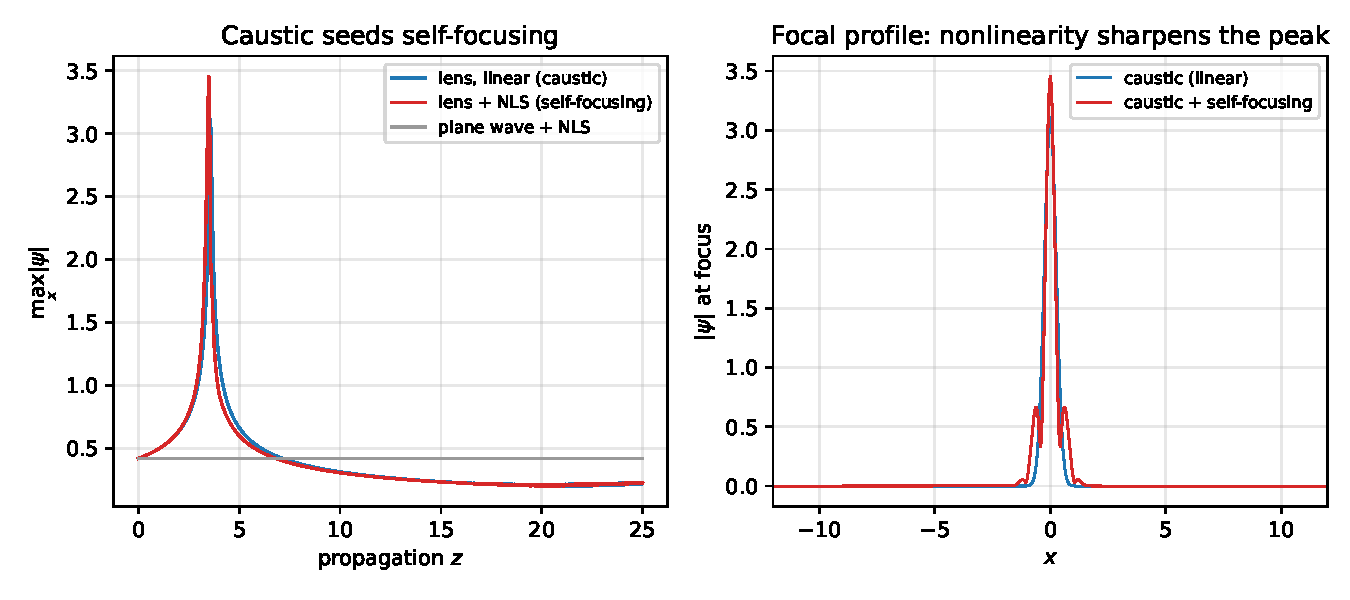
\includegraphics[width=.94\textwidth]{fig_caustic_mi.pdf}
\caption{A linear caustic seeds nonlinear self-focusing (focusing NLS, lens-seeded beam). Left: the peak
amplitude---the lens focuses a weak flat input ${\sim}7\times$ (caustic), the nonlinearity adds a further
${\sim}11\%$, while the lensless plane wave stays flat. Right: at the focus the nonlinearity sharpens and
heightens the peak.}\label{fig:caustic_mi}
\end{figure}

\begin{figure}[ht]\centering
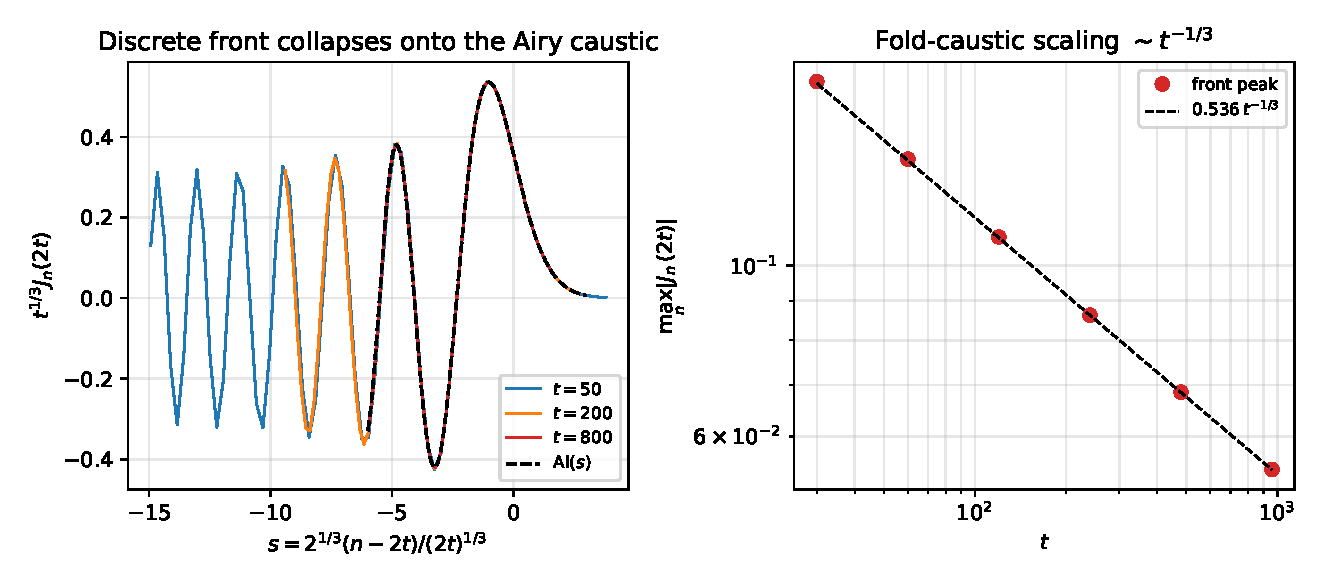
\includegraphics[width=.92\textwidth]{fig_caustic.pdf}
\caption{The discrete-Schr\"odinger front as a fold caustic. Left: the rescaled fronts $t^{1/3}J_n(2t)$
for $t=50,200,800$ collapse onto the Airy function $\mathrm{Ai}(s)$, $s=2^{1/3}(n-2t)/(2t)^{1/3}$
(Eq.~\eqref{eq:airy}). Right: the front peak follows the universal fold scaling
$0.536\,t^{-1/3}$.}\label{fig:caustic}
\end{figure}

\begin{figure}[ht]\centering
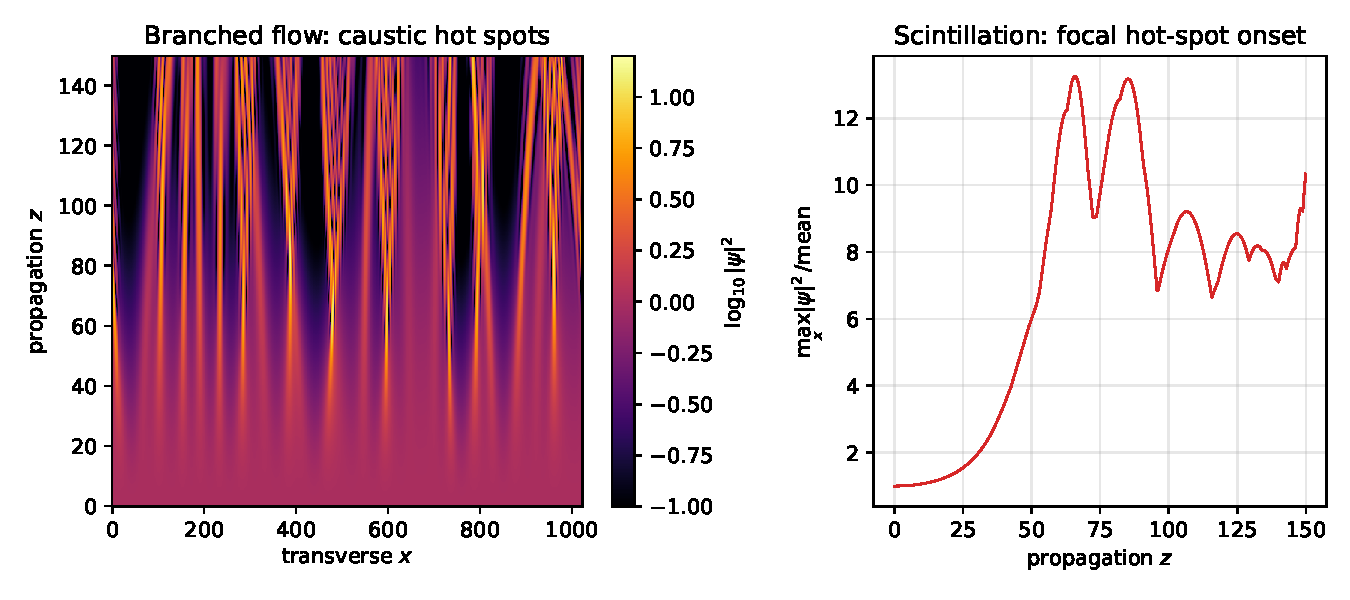
\includegraphics[width=.94\textwidth]{fig_branched.pdf}
\caption{Branched flow of a wave in a weak random current (paraxial model). Left: a uniform incident
wave ($z=0$) develops bright caustic filaments and focal hot spots as it propagates. Right: the
scintillation index rises from $1$ to ${\sim}13$ at the first focal distance---the linear, refractive
route to a rogue hot spot.}\label{fig:branched}
\end{figure}


\section{Discussion}

The ring and the Dirichlet segment realize the same mechanism---constructive phase alignment of a
logarithmically weighted family of modes---through different arithmetic. On the segment the
frequencies $2\sin(\pi k/2N)$ lie in $\Q(\zeta_{4N})$; on the ring $2\sin(\pi r/N)\in\Q(\zeta_{2N})$,
with the twofold degeneracy $\omega_r=\omega_{N-r}$ that halves the number of independent phases and
(as the time-averaged $\mathrm{RMS}_t|G_N(0,\cdot)|=\sqrt{(N^2-1)/(12N^2)}\to1/\sqrt{12}$ shows) doubles the typical energy
relative to a naive independent count. The growth constant $1/\pi$ is identical on the classes where
the frequencies are rationally independent; the composite defect is a sub-torus phenomenon that, on the
evidence of Section~\ref{sec:exact}, does not lower the order below $\Theta(\ln N)$ (Conjecture~\ref{conj:order}).

The discrete Schr\"odinger equation occupies the opposite extreme. Its phases are governed by
$\lambda_r=2-2\cos(2\pi r/N)$, which lie in the real cyclotomic field $\Q(\zeta_N)^+$ and always
satisfy the affine relation $\sum_r\lambda_r=2N$. Unitarity caps the response to a localized state,
and the genuine amplification---ballistic, of order $\sqrt N$---is carried by spread-out
$\ell^\infty$ data. The contrast $\ln N$ (wave) versus $\sqrt N$ (Schr\"odinger) traces back to the
difference between $\sqrt{\lambda_r}$ and $\lambda_r$ in the propagator phase.

\medskip
\noindent\textbf{GLT context.} The sequence $\{\LN\}$ is a circulant---hence locally Toeplitz---instance
of a Generalized Locally Toeplitz (GLT) sequence~\cite{GLT} with symbol $f(\theta)=4\sin^2(\theta/2)$.
The spectral-zeta density \eqref{eq:zeta-density} and the Szeg\H{o} asymptotics are the GLT spectral
distribution specialized to this symbol; beyond the uniform $d$-torus settled in
Section~\ref{sec:dim}, the GLT calculus extends the \emph{asymptotic spectral-distribution} statements
(the Szeg\H{o}/zeta density) to variable-coefficient lattices (non-uniform masses) and anisotropic or
graph Laplacians; the \emph{arithmetic} results---the cyclotomic ranks, the mod-$4$ criterion, and the
reachability of the ceiling---do not transfer automatically and are the natural setting for future work.

\medskip
\noindent\textbf{A different face of energy concentration.} The discrete Laplacian concentrates energy
beyond wave dynamics. In the dielectric-breakdown (Laplacian-growth) model of lightning~\cite{NPW}, the
electrostatic potential solves the discrete Laplace equation $\LN^{(2)}\phi=0$ off the leader, which
advances toward the strongest field; the result is a branched, fractal discharge (fractal dimension
$\approx1.5$ in our run) with the field---and the energy---concentrated at its tips, the same operator
and branched morphology as the refractive caustics of Section~\ref{sec:caustic} but by a distinct
(elliptic, dissipative) mechanism (Figure~\ref{fig:lightning}, \texttt{verify\_laplacian\_lightning.py}).

\begin{figure}[ht]\centering
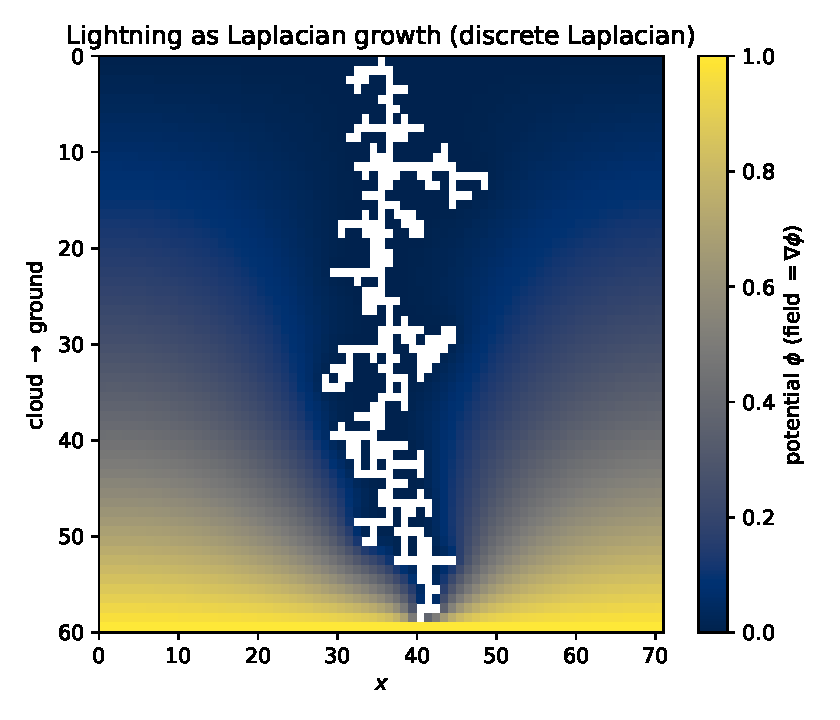
\includegraphics[width=.56\textwidth]{fig_lightning.pdf}
\caption{Lightning as Laplacian growth: the leader (white) advances cloud-to-ground where the field is
strongest, the potential $\phi$ solving the discrete Laplace equation $\LN^{(2)}\phi=0$ off it. A
branched fractal discharge with the energy concentrated at its tips---energy concentration on the same
discrete Laplacian, electrostatically.}\label{fig:lightning}
\end{figure}

\medskip\noindent\textbf{Limitations.} We mark the boundaries of what is established. (i)~The quantitative
law $A_N=\Theta(\ln N)$ is \emph{proved} only on the prime, $2^m$, and $2p$ classes; for general $N$ only
$A_N\le U_N$ is rigorous, and the matching lower bound (Conjecture~\ref{conj:order}) is open---the
obstruction is the destructive interference of the out-of-prefix modes, so the prefix budget
$L_{\mathrm{pre}}$ is heuristic, not a proven bound. (ii)~The ceiling criterion
(Theorem~\ref{thm:ceiling}) is exact, but whether any \emph{composite} $N$ satisfies it is verified only
to $N\le160$ (none does); the algebraic value of $A_N$ for individual composite $N$ is computed, not
bounded in closed form. (iii)~The Schr\"odinger order $B_N=\Theta(\sqrt N)$ is proved, but the optimal
constant is open: $\liminf_N B_N/\sqrt N\ge0.6086$ and $\limsup_N B_N/\sqrt N\le1$, with existence of the
limit unknown. The segment constant $C=4/\pi^2$ (Section~\ref{sub:filimonov}) is \emph{not} ours: it is the
published Myshkis--Filimonov value~\cite[Thm.~2]{MF03}, which the Schr\"odinger ceiling inherits because the
two ceilings coincide. (iv)~The segment rank \eqref{eq:segrank} is verified to $N\le30$ and conjectured in
general. (v)~Part~II is \emph{computational and exploratory}: its rigorous statements (the Hamiltonian
conservation laws, Proposition~\ref{prop:dnls-cons}, and the linear modulational band,
Proposition~\ref{prop:mi}) are classical, while the genuinely hard nonlinear results---existence and
stability of discrete breathers, the precise dynamical self-trapping threshold, and the route to
chaos---are simulated, not proved. (vi)~The
supremum $A_N$ is an \emph{infinite-time} quantity; the amplitude reached on any physical horizon is
Diophantine-limited (Section~\ref{sec:reach}). Proved statements are separated throughout from numerical
evidence and from the conjectures, and every quantitative claim is reproduced by a standalone script.

\section{Open problems}

\begin{enumerate}
\item Prove $A_N=\Theta(\ln N)$ (Conjecture~\ref{conj:order}), and the sharp constant
$A_N\sim\tfrac1\pi\ln N$, for \emph{general} $N$. Both are rigorous on the prime, $2^m$, and $N=2p$
classes (Theorems~\ref{thm:prime}--\ref{thm:two}, Proposition~\ref{prop:2p}); for general $N$ only the
upper bound $A_N\le U_N$ is proved, and the lower bound is open (the obstruction is the control of the
out-of-prefix interference, Observation~\ref{obs:prefix}). Numerically the defect closes,
$A_N/U_N\to1$ (e.g.\ $0.92\to0.999$ along $N=2p$ up to $N=46$), so the constant appears universally
$1/\pi$; certified numerical brackets for individual composite $N$ follow from the Lasserre moment--SOS
hierarchy (Section~\ref{sec:exact}).
\item Determine the exact constant $\lim_{N\to\infty}B_N/\sqrt N$ for the Schr\"odinger propagator. The
order $B_N=\Theta(\sqrt N)$ is now settled (Theorems~\ref{thm:schr},~\ref{thm:schr-lower}): the lower
bound $\liminf_N B_N/\sqrt N\ge\tfrac12 c_0\approx0.6086$ ($c_0=(2/\pi)^{3/2}B(\tfrac12,\tfrac34)$) comes
from the unwrapped Bessel front at $t=N/8$, the upper bound $1$ from unitarity, and a $t$-scan
(including the structured candidate times $t=\pi a/N$) gives a largest scanned ratio $\approx0.88$--$0.96$;
whether $\lim_N B_N/\sqrt N$ exists (with $\liminf\ge0.6086$, $\limsup\le1$) is an almost-periodic /
Gauss-sum question
(\texttt{verify\_open\_problems.py}).
\item A rigorous nonlinear theory of the discrete NLS \eqref{eq:dnls} on the ring
(Section~\ref{sec:rogue}): existence and stability of discrete breathers, the role of the $\LN$
spectrum in the modulational-instability band, and a Klein--Gordon analogue.
\item The multidimensional nonlinear large wave (Section~\ref{sec:highd}): existence, stability, and
the energy threshold of the $2$D/$3$D discrete breathers, and the long-wave dynamics in the
Zakharov--Kuznetsov regime~\cite{ZakharovKuznetsov}---a nonlinear counterpart to the dimensional
threshold of Section~\ref{sec:dim}.
\item Whether the statistics of the thermalizing lattice are governed by the weak-turbulence
(Kolmogorov--Zakharov) wave kinetic description~\cite{ZakharovLvovFalkovich,DengHani}, and the rate of
approach to energy equipartition.
\item The interplay of the two energy-concentration routes (Section~\ref{sec:caustic}): when does a
linear refractive caustic raise the local steepness enough to trigger the modulational instability of
Section~\ref{sec:rogue}, and what rogue-amplitude statistics result on the lattice?
\end{enumerate}

\appendix

\section{Derivation of the ring spectrum}\label{app:spectrum}
Seeking $\LN\varphi=\lambda\varphi$ with $\varphi_{j+N}=\varphi_j$, the constant-coefficient recurrence
$-\varphi_{j+1}+(2-\lambda)\varphi_j-\varphi_{j-1}=0$ has characteristic equation
$p^2-(2-\lambda)p+1=0$ with $p_1p_2=1$ (Vieta). Nontrivial bounded solutions require conjugate roots
$p_{1,2}=\eu^{\pm\mathrm i\theta}$ on the unit circle, so $2-\lambda=2\cos\theta$. The periodicity
$\varphi_{j+N}=\varphi_j$ forces $\eu^{\mathrm i\theta N}=1$, i.e.\ $\theta=2\pi r/N$, whence
\[
  \lambda_r=2-2\cos\tfrac{2\pi r}{N}=4\sin^2\tfrac{\pi r}{N},\qquad
  \varphi^{(r)}_j=\eu^{2\pi\mathrm i rj/N}\ \ (r=0,\dots,N-1),
\]
with the real basis $1,\ \cos\frac{2\pi rj}{N},\ \sin\frac{2\pi rj}{N},\ (-1)^j$. Each level is doubly
degenerate, $\lambda_r=\lambda_{N-r}$, except $\lambda_0=0$ and---for even $N$---$\lambda_{N/2}=4$.
The Dirichlet segment is identical with the closure $\sin\bigl(\theta(N{+}1)\bigr)=0$, giving
$\theta=\pi k/(N{+}1)$ and $\lambda^{\mathrm{Dir}}_k=4\sin^2\frac{\pi k}{2(N+1)}$ (all simple).

\section{Asymptotics of the cosecant sum}\label{app:bernoulli}
We derive Lemma~\ref{lem:asym}. The sum $S_N=\sum_{r=1}^{N-1}\csc(\pi r/N)$ has reciprocal singularities
at \emph{both} ends---$\csc(\pi r/N)\sim N/(\pi r)$ as $r\to0$ and $\sim N/(\pi(N-r))$ as $r\to N$---which
we subtract symmetrically:
\[
  S_N=\frac N\pi\sum_{r=1}^{N-1}\Bigl(\frac1r+\frac1{N-r}\Bigr)
      +\sum_{r=1}^{N-1}\underbrace{\Bigl[\csc\tfrac{\pi r}N-\frac N{\pi r}-\frac N{\pi(N-r)}\Bigr]}_{=\,R(r/N)} .
\]
The first sum is $\tfrac{2N}\pi H_{N-1}=\tfrac{2N}\pi(\ln N+\gamma)+O(1/N)$. The integrand
$R(x)=\csc\pi x-\tfrac1{\pi x}-\tfrac1{\pi(1-x)}$ is smooth and bounded on $[0,1]$ (both poles cancel), so
the second sum is a Riemann sum, $\sum_{r=1}^{N-1}R(r/N)=N\!\int_0^1\!R(x)\,dx+O(1)$, and the integral is
elementary (using $\int\csc\pi x\,dx=\tfrac1\pi\ln\tan\tfrac{\pi x}2$):
\[
  \int_0^1\!R(x)\,dx=\frac1\pi\Bigl[\ln\frac{(1-x)\tan(\pi x/2)}{x}\Bigr]_0^1=\frac2\pi\ln\frac2\pi .
\]
Hence the leading asymptotics, with additive constant $\tfrac1\pi(\gamma+\ln\tfrac2\pi)=0.03999\ldots$,
\[
  S_N=\frac{2N}\pi\Bigl(\ln N+\gamma+\ln\tfrac2\pi\Bigr)+O(1),
  \qquad U_N=\frac{S_N}{2N}=\frac1\pi\ln N+\frac1\pi\Bigl(\gamma+\ln\tfrac2\pi\Bigr)+o(1).
\]
The next correction is the Euler--Maclaurin endpoint term of $R$ (a Bernoulli-$B_2$ contribution); it is
even in $1/N$ and evaluates to
\[
  U_N=\frac1\pi\ln N+\frac1\pi\Bigl(\gamma+\ln\tfrac2\pi\Bigr)-\frac{\pi}{72}\,\frac1{N^2}+O(N^{-4}),
  \qquad -\frac{\pi}{72}=-\frac{\zeta(2)}{12\pi},
\]
confirmed to six digits by Richardson extrapolation ($a_2=-0.043633$). The correction is thus tied to the
same $\zeta(2)$ that governs $\zeta_{\LN}(2)$ in Section~\ref{sec:zeta}; see
\texttt{verify\_asymptotic\_corrections.py}.

\section{Reproducible code}\label{app:code}
Every quantitative claim is reproduced by a standalone script run with \texttt{uv run} (inline
PEP~723 dependencies); the figures are generated by \texttt{make\_figures.py}, and the core routines
(ring spectrum, Bohr ceiling, cyclotomic ranks, Schr\"odinger kernel) live in a tested package
\texttt{large\_wave\_effect} with a \texttt{pytest} suite. The scripts are listed in
Section~\ref{sec:repro}. The complete repository---scripts, section sources, and figures---is public at
\url{https://github.com/ilgrad/large-wave-effect}, where every \texttt{verify\_*.py} passes.

\begin{thebibliography}{99}
\bibitem{Bohr} H.~Bohr, \emph{Almost Periodic Functions}, Chelsea, New York, 1947.
\bibitem{Weyl} H.~Weyl, \emph{\"Uber die Gleichverteilung von Zahlen mod.\ Eins}, Math.\ Ann.\ \textbf{77} (1916), 313--352.
\bibitem{Niven} I.~Niven, \emph{Irrational Numbers}, Carus Math.\ Monographs \textbf{11}, MAA, 1956.
\bibitem{CJ} J.~H.~Conway and A.~J.~Jones, \emph{Trigonometric Diophantine equations (on vanishing sums of roots of unity)}, Acta Arith.\ \textbf{30} (1976), 229--240.
\bibitem{Watson} G.~N.~Watson, \emph{A Treatise on the Theory of Bessel Functions}, Cambridge Univ.\ Press, 1944.
\bibitem{Gray} R.~M.~Gray, \emph{Toeplitz and Circulant Matrices: A Review}, Found.\ Trends Commun.\ Inf.\ Theory \textbf{2} (2006), 155--239.
\bibitem{Lasserre} J.~B.~Lasserre, \emph{Global optimization with polynomials and the problem of moments}, SIAM J.\ Optim.\ \textbf{11} (2001), 796--817.
\bibitem{Levinson} N.~Levinson, \emph{The Wiener RMS error criterion in filter design and prediction}, J.\ Math.\ Phys.\ \textbf{25} (1947), 261--278.
\bibitem{Durbin} J.~Durbin, \emph{The fitting of time-series models}, Rev.\ Inst.\ Internat.\ Statist.\ \textbf{28} (1960), 233--244.
\bibitem{Trench} W.~F.~Trench, \emph{An algorithm for the inversion of finite Toeplitz matrices}, J.\ SIAM \textbf{12} (1964), 515--522.
\bibitem{GS} I.~C.~Gohberg, A.~A.~Semencul, \emph{On the inversion of finite Toeplitz matrices and their continuous analogues}, Mat.\ Issled.\ \textbf{7} (1972), 201--223.
\bibitem{GrenanderSzego} U.~Grenander, G.~Szeg\H{o}, \emph{Toeplitz Forms and Their Applications}, Univ.\ of California Press, 1958.
\bibitem{BS} A.~B\"ottcher, B.~Silbermann, \emph{Introduction to Large Truncated Toeplitz Matrices}, Springer, 1999.
\bibitem{GVL} G.~H.~Golub, C.~F.~Van Loan, \emph{Matrix Computations}, 4th ed., Johns Hopkins Univ.\ Press, 2013.
\bibitem{GLT} C.~Garoni, S.~Serra-Capizzano, \emph{Generalized Locally Toeplitz Sequences: Theory and Applications}, Vol.~I, Springer, 2017.
\bibitem{AAW} I.~V.~Andrianov, J.~Awrejcewicz, D.~Weichert, \emph{Improved continuous models for discrete media}, Math.\ Probl.\ Eng.\ \textbf{2010} (2010), art.\ 986242. \texttt{doi:10.1155/2010/986242}.
\bibitem{Longhi} S.~Longhi, \emph{Kramers--Kronig potentials for the discrete Schr\"odinger equation}, Phys.\ Rev.\ A \textbf{96} (2017), 042106. \texttt{doi:10.1103/PhysRevA.96.042106}.
\bibitem{Gradina12} Ilia Gradina, \emph{Solving the basic problems of linear algebra for Toeplitz matrices}, term paper, MIIT, 2012 (unpublished).
% Filimonov-group references below verified via Crossref (DOIs included); MF03 from info/ PDF.
\bibitem{MF03} A.~D.~Myshkis, A.~M.~Filimonov, \emph{About the string with beads}, Mat.\ Fiz.\ Anal.\ Geom.\ \textbf{10} (2003), no.~3, 301--306. (Segment $\ln$-asymptotics.)
\bibitem{KMF} P.~F.~Kurchanov, A.~D.~Myshkis, A.~M.~Filimonov, \emph{Vibrations of rolling stock and a theorem of Kronecker}, J.~Appl.\ Math.\ Mech.\ \textbf{55} (1991), no.~6, 870--876 (Russian original: Prikl.\ Mat.\ Mekh.\ \textbf{55}(6), 989--995). \texttt{doi:10.1016/0021-8928(91)90140-P}.
\bibitem{FKM91} A.~M.~Filimonov, P.~F.~Kurchanov, A.~D.~Myshkis, \emph{Some unexpected results in the classical problem of vibration of the string with $n$ beads when $n$ is large}, C.~R.~Acad.\ Sci.\ Paris S\'er.~I \textbf{313} (1991), no.~13, 961--965. (Cited from the lineage list of~\cite{F23}; not consulted directly.)
\bibitem{F92} A.~M.~Filimonov, \emph{Some unexpected results on the classical problem of vibrations of the string with $N$ beads. The case of multiple frequencies}, C.~R.~Acad.\ Sci.\ Paris S\'er.~I \textbf{315} (1992), no.~8, 957--961. (Cited from the lineage list of~\cite{F23}; not consulted directly.)
\bibitem{FM98} A.~M.~Filimonov, A.~D.~Myshkis, \emph{Asymptotic estimate of solution of one mixed difference--differential equation of oscillations theory}, J.~Difference Equ.\ Appl.\ \textbf{4} (1998), no.~1, 13--16. \texttt{doi:10.1080/10236199808808125}. (First $\ln$-growth result; cited from~\cite{MF03}.)
\bibitem{FMM} A.~M.~Filimonov, X.~Mao, S.~Maslov, \emph{Splash effect and ergodic properties of solutions of the classical difference--differential equation}, J.~Difference Equ.\ Appl.\ \textbf{6} (2000), no.~3, 319--328. \texttt{doi:10.1080/10236190008808231}.
\bibitem{FM} A.~M.~Filimonov, A.~D.~Myshkis, \emph{On properties of the large wave effect in the classical problem of bead string vibration}, J.~Difference Equ.\ Appl.\ \textbf{10} (2004), no.~13--15, 1171--1175. \texttt{doi:10.1080/10236190410001652757}.
\bibitem{F23} A.~M.~Filimonov, \emph{Sufficient conditions for the large wave phenomenon in the Schr\"odinger equation with discrete spatial variable}, J.~Math.\ Sci.\ \textbf{269} (2023), no.~6, 792--795. \texttt{doi:10.1007/s10958-023-06316-1}.
\bibitem{Zhukovsky} N.~E.~Zhukovsky, \emph{Collected Works} (the railway train start-up problem), vol.~VIII, 1937 (classical; not DOI-indexed).

\bibitem{Zakharov} V.~E.~Zakharov, \emph{Stability of periodic waves of finite amplitude on the surface of a deep fluid}, J.~Appl.\ Mech.\ Tech.\ Phys.\ \textbf{9} (1968), 190--194. \texttt{doi:10.1007/BF00913182}.
\bibitem{ZakharovShabat} V.~E.~Zakharov, A.~B.~Shabat, \emph{Exact theory of two-dimensional self-focusing and one-dimensional self-modulation of waves in nonlinear media}, Zh.\ Eksp.\ Teor.\ Fiz.\ \textbf{61} (1971), 118--134 [Sov.\ Phys.\ JETP \textbf{34} (1972), 62--69].
\bibitem{ZakharovFaddeev} V.~E.~Zakharov, L.~D.~Faddeev, \emph{Korteweg--de Vries equation: a completely integrable Hamiltonian system}, Funct.\ Anal.\ Appl.\ \textbf{5} (1971), 280--287. \texttt{doi:10.1007/BF01086739}.
\bibitem{ZakharovOstrovsky} V.~E.~Zakharov, L.~A.~Ostrovsky, \emph{Modulation instability: the beginning}, Phys.\ D \textbf{238} (2009), 540--548. \texttt{doi:10.1016/j.physd.2008.12.002}.
\bibitem{ZakharovKuznetsov} V.~E.~Zakharov, E.~A.~Kuznetsov, \emph{On three-dimensional solitons}, Zh.\ Eksp.\ Teor.\ Fiz.\ \textbf{66} (1974), 594--597 [Sov.\ Phys.\ JETP \textbf{39} (1974), 285--286].
\bibitem{ZakharovLvovFalkovich} V.~E.~Zakharov, V.~S.~L'vov, G.~Falkovich, \emph{Kolmogorov Spectra of Turbulence~I: Wave Turbulence}, Springer, 1992.
\bibitem{DengHani} Y.~Deng, Z.~Hani, \emph{Full derivation of the wave kinetic equation}, Invent.\ Math.\ \textbf{233} (2023), 543--724. \texttt{doi:10.1007/s00222-023-01189-2}.
\bibitem{BerryUpstill} M.~V.~Berry, C.~Upstill, \emph{Catastrophe optics: morphologies of caustics and their diffraction patterns}, Prog.\ Opt.\ \textbf{18} (1980), 257--346. \texttt{doi:10.1016/S0079-6638(08)70215-4}.
\bibitem{WhiteFornberg} B.~S.~White, B.~Fornberg, \emph{On the chance of freak waves at sea}, J.~Fluid Mech.\ \textbf{355} (1998), 113--138. \texttt{doi:10.1017/S0022112097007751}.
\bibitem{Lavrenov} I.~V.~Lavrenov, \emph{The wave energy concentration at the Agulhas current off South Africa}, Nat.\ Hazards \textbf{17} (1998), 117--127. \texttt{doi:10.1023/A:1007978326982}.
\bibitem{YingHeller} L.~H.~Ying, Z.~Zhuang, E.~J.~Heller, L.~Kaplan, \emph{Linear and nonlinear rogue wave statistics in the presence of random currents}, Nonlinearity \textbf{24} (2011), R67--R87. \texttt{doi:10.1088/0951-7715/24/11/R01}.
\bibitem{ZakharovShamin} V.~E.~Zakharov, R.~V.~Shamin, \emph{Probability of the occurrence of freak waves}, JETP Lett.\ \textbf{91} (2010), 62--65. \texttt{doi:10.1134/S0021364010020025}.
\bibitem{Slunyaev} A.~V.~Slunyaev, D.~E.~Pelinovsky, E.~N.~Pelinovsky, \emph{Rogue waves in the sea: observations, physics, and mathematics}, Phys.\ Usp.\ \textbf{66} (2023), 148--172. \texttt{doi:10.3367/UFNe.2021.08.039038}.
\bibitem{NPW} L.~Niemeyer, L.~Pietronero, H.~J.~Wiesmann, \emph{Fractal dimension of dielectric breakdown}, Phys.\ Rev.\ Lett.\ \textbf{52} (1984), 1033--1036. \texttt{doi:10.1103/PhysRevLett.52.1033}.
\bibitem{BenjaminFeir} T.~B.~Benjamin, J.~E.~Feir, \emph{The disintegration of wave trains on deep water. Part 1. Theory}, J.~Fluid Mech.\ \textbf{27} (1967), 417--430. \texttt{doi:10.1017/S002211206700045X}.
\bibitem{Peregrine} D.~H.~Peregrine, \emph{Water waves, nonlinear Schr\"odinger equations and their solutions}, J.~Austral.\ Math.\ Soc.\ Ser.~B \textbf{25} (1983), 16--43. \texttt{doi:10.1017/S0334270000003891}.
\bibitem{Akhmediev} N.~N.~Akhmediev, V.~I.~Korneev, \emph{Modulation instability and periodic solutions of the nonlinear Schr\"odinger equation}, Theoret.\ Math.\ Phys.\ \textbf{69} (1986), 1089--1093. \texttt{doi:10.1007/BF01037866}.
\bibitem{MacKayAubry} R.~S.~MacKay, S.~Aubry, \emph{Proof of existence of breathers for time-reversible or Hamiltonian networks of weakly coupled oscillators}, Nonlinearity \textbf{7} (1994), 1623--1643. \texttt{doi:10.1088/0951-7715/7/6/006}.
\bibitem{KharifPelinovsky} C.~Kharif, E.~Pelinovsky, \emph{Physical mechanisms of the rogue wave phenomenon}, Eur.\ J.\ Mech.\ B/Fluids \textbf{22} (2003), 603--634. \texttt{doi:10.1016/j.euromechflu.2003.09.002}.
\bibitem{Solli} D.~R.~Solli, C.~Ropers, P.~Koonath, B.~Jalali, \emph{Optical rogue waves}, Nature \textbf{450} (2007), 1054--1057. \texttt{doi:10.1038/nature06402}.
\bibitem{Onorato} M.~Onorato, S.~Residori, U.~Bortolozzo, A.~Montina, F.~T.~Arecchi, \emph{Rogue waves and their generating mechanisms in different physical contexts}, Phys.\ Rep.\ \textbf{528} (2013), 47--89. \texttt{doi:10.1016/j.physrep.2013.03.001}.
\end{thebibliography}

\end{document}
